% REMEMBER: You must not plagiarise anything in your report. Be extremely careful.

\documentclass{l4proj}
%
% put any additional packages here
%
\usepackage{float}
\usepackage{pgf-pie}
\usepackage{graphicx}

\begin{document}

%==============================================================================
%% METADATA
\title{Cyclist-Autonomous Vehicle Interaction: Enhancing Road Safety through an Augmented Reality Prototype}
\author{Cameron McDonald}
\date{March 29, 2024}

\maketitle

%==============================================================================
%% ABSTRACT
\begin{abstract}
As the introduction of autonomous vehicles onto public roads draws closer, ensuring safe interactions with cyclists is imperative. This study aims to address the communication gap between cyclists and autonomous vehicles by designing and evaluating an augmented reality prototype. The prototype aims to enhance cyclists awareness of autonomous vehicles' intent on the road. Through a survey, cyclists opinions on augmented reality technology and interaction design preferences were gathered.

Results indicated a range of perspectives amongst cyclists regarding the potential of augmented reality to improve road safety. Those in favour of the idea had concerns over the capabilities of the headsets, whilst those against the idea suggested a move for separation of cyclists and autonomous vehicles, should the vehicles not been deemed safe. Future research should focus on real-world testing and further investigation of cyclists attitude towards autonomous vehicles.

This study addresses the importance of solving communication challenges between cyclists and autonomous vehicles to ensure the safety of everyone as we move towards the autonomous era.
    \vskip 0.5em
\end{abstract}

%==============================================================================

% EDUCATION REUSE CONSENT FORM
% If you consent to your project being shown to future students for educational purposes
% then insert your name and the date below to  sign the education use form that appears in the front of the document. 
% You must explicitly give consent if you wish to do so.
% If you sign, your project may be included in the Hall of Fame if it scores particularly highly.
%
% Please note that you are under no obligation to sign 
% this declaration, but doing so would help future students.
%
%\def\consentname {My Name} % your full name
%\def\consentdate {20 March 2018} % the date you agree
%
\educationalconsent


%==============================================================================
\tableofcontents

%==============================================================================
%% Notes on formatting
%==============================================================================
% The first page, abstract and table of contents are numbered using Roman numerals and are not
% included in the page count. 
%
% From now on pages are numbered
% using Arabic numerals. Therefore, immediately after the first call to \chapter we need the call
% \pagenumbering{arabic} and this should be called once only in the document. 
%
% The first Chapter should then be on page 1. You are allowed 40 pages for a 40 credit project and 20 pages for a 
% 20 credit report. This includes everything numbered in Arabic numerals (excluding front matter) up
% to but excluding the appendices and bibliography.
%
% You must not alter text size (it is currently 10pt) or alter margins or spacing.
%
%
%==================================================================================================================================
%
% IMPORTANT
% The chapter headings here are **suggestions**. You don't have to follow this model if
% it doesn't fit your project. Every project should have an introduction and conclusion,
% however. 
%
%==================================================================================================================================

\chapter{Introduction}

% reset page numbering. Don't remove this!
\pagenumbering{arabic}

\section{Introduction}
In recent years, cycling has faced a surge in popularity worldwide as it has been widely recognised as a healthy and sustainable method of transportation. According to \citep{statista} in 2022 alone, 7.61 million people took part in cycling here in the United Kingdom. Everywhere from bustling urban streets to beautiful countryside paths, cyclists can be found enjoying the freedom of two wheels whether it may be for travelling to work, getting fit or simply as a means of transport. However, in contrast to the growing popularity of cycling comes a pressing concern; safety on the road. Despite the many benefits to health and the environment that cycling boasts, it remains a dangerous activity particularly due to interactions with motorised vehicles when on the road.

\section{Background and Context}
Cyclists face a whole host of challenges when navigating through traffic, anything from negotiating right of way at intersections to maneuvering through congested lanes and avoiding vehicles many times their size. These challenges can be made worse due to a lack of designated cycling infrastructure and the vulnerability of cyclists when compared to the motorised vehicles they share the road with. With all this in mind, ensuring the safety of cyclists on the road has become an urgent and imperative task for road planners, council members and engineers alike.

\section{Problem Statement}
At the forefront of the issue regarding the safety of cyclists on public roads is the communication gap between cyclists and the drivers of vehicles. There is often a level of ambiguity surrounding right of way, signalling intentions and interpreting non-verbal cues which may lead to misunderstandings and, in some cases, dangerous collisions between the two parties. Approaches to mitigate these risks, such as traffic signage, hand signals and vehicle signals have, time and time again, proven inadequate in addressing the issue of real-time interaction between cyclists and drivers. This issue becomes even more prevalent when looking into the near to distant future with the rise of autonomous vehicles and the lack of road safety technology currently available to the public.

\section{Objective and Scope of the Study}
This project aims to explore innovative solutions to improve the safety of cyclists on the road and focuses specifically on the potential implementation of augmented reality technology in order to enhance road safety. By leveraging the ability to create applications for augmented reality, I seek to improve the communication between cyclists and vehicles, whether autonomous or not, by providing clearer visual cues in the form of graphical overlays. The study itself, will look into opinion amongst cyclists about augmented reality and showcase a prototype in order to gain feedback on the design choices.

\section{Significance of Research}
The findings of this research have the potential to hold significant implications for the future of transport engineering, human-computer interaction, the planning of urban areas and the design of autonomous vehicles. By addressing the current communication challenges in cyclist-vehicle interactions, my study contributes towards an ongoing effort to improve the safety of all road users and provides insight into the future of transport and the potential implementation of technology.

\section{Overview of the Dissertation Structure}
The subsequent chapters of this dissertation cover the entire scope of my project by reviewing current existing literature on the topic of cyclist-vehicle interaction, looking into the analysis of the problem, the design process the project went through, the implementation of the project and finally the feedback I received from the evaluation stage.

%==================================================================================================================================

\chapter{Background}

\section{Overview}

Despite the popularity of cycling and the looming future of autonomous vehicles, there has been a very small amount of studies that have taken place in order to look at the interactions between the two parties. Instead, the majority of research has looked into the interactions between autonomous vehicles and pedestrians. The research that has taken place prior to this study has proven instrumental in the design and implementation of this project.

\section{Keep it Real \citep{keep_it_real}}

As previously specified, the level of research into driver-cyclist interaction that can inform interaction design between autonomous vehicles and cyclists, is low to none existent. This research paper aims to shine a light on the matter and provide designers with the knowledge they need in order to make decisions on the future of interactions on the road.

The goal of this study is to fill the gap in the research and to do so it defines two different questions it answers 'How do the messages, social cues, implicit cues and on-vehicle signals that cyclists and drivers exchange differ between traffic scenarios?' and 'How does cyclist gaze behaviour toward vehicle and traffic control features differ between traffic scenarios?'.

In order to answer both questions, two different studies were conducted. The first study, which answers the first research question, had observers filling in online forms at five different locations. The information they obtained from the observers included site conditions, number of encounters/interactions and the messages, social cues and implicit cues that were used in the communication between the vehicle and the cyclist. The research concluded that, in the study, 55.8 percent of encounters between cyclists and vehicles resulted in interactions. The research also concluded that interactions occurred more commonly, in the study, when showing cyclist awareness in lane merging and negotiating right of way at uncontrolled intersections. In terms of the interactions, the different types of social and implicit cues used by both the driver and cyclist in each of the five scenarios varied heavily, however drivers were more likely to face their head towards cyclists and come to a complete stop at uncontrolled intersections. In contrast to the drivers social and implicit cues, cyclists tended to be a bit more varied depending on the scenario but some key cues emerged from the research, mainly cyclists tended to face their head towards the driver when lane merging and accelerated at uncontrolled intersections. Whilst the research obtained from answering the first research question does not directly correlate with my project, there are however some important takeaways from it that can be used in the designing of the projects solution. Understanding the way in which cyclists and drivers interact can shed light on the future of cyclist-autonomous vehicle interaction.

The second study that was conducted and detailed in 'Keep It Real', in order to answer the second research question, focused on a naturalistic study of cyclists when out riding on public roads. Cyclists were equipped with eye tracking glasses and a bike computer in order to obtain GPS, video footage and gaze data from the cyclists. Prior to the study, areas of interest were defined on vehicles which allowed the gaze data to be put into context and provide information on the area in which cyclists focused on the most. Derived from the results of this study, a map of gaze fixation on vehicles and road signs/signals was created which shows the distribution of cyclists gaze depending on the scenario out on public roads. The maps created show a large amount of cyclists gaze was concentrated on the front or the side of vehicles, in some scenarios gaze was fixated more on road signs and signals rather than on the vehicle, for example at controlled intersections. The research into cyclists gaze conducted in this paper will no doubt shape the future of the design of interactions between cyclist and autonomous vehicles.

The work concludes by offering an overall discussion and a look into implications for autonomous vehicle interactions based off of the research carried out. Within this conclusion is a section on potential design choices for creating a medium in which cyclists and vehicles can interact with the use augmented reality glasses. The design suggestion focuses on the use of a traffic light coloured system on the side of a vehicle in order to interact with cyclists over the discussion of right of way. The design that I use for this project takes notes from this suggestion and is heavily influenced by the work carried out in this paper.

\section{Light it Up \citep{light_it_up}}

'Light it Up' investigates the effectiveness of External Human Machine Interfaces, also known as eHMIs, as a replacement for the traditional social signals displayed by a driver. It offers an introduction to eHMIs as a solely vehicle based interaction method that would require no technology to be worn by the cyclist out on public roads. The paper itself looks into the effectiveness of eHMIs when communicating with a cyclist to state the autonomous vehicles intention and awareness of the cyclist. To gather research into eHMIs effectiveness, two research questions are defined. The first, 'How versatile, acceptable and usable are eHMIs in terms of cyclist perception?' and the second, 'How versatile, acceptable and usable are eHMIs in terms of cycling behaviour?'. To answer the two different research questions, two different studies were performed.

The initial study utilises virtual reality technology in order to gain feedback on eHMIs that have been designed. Participants were setup on an indoor bicycle with the back wheel attached to a trainer, a Meta Quest Pro headset with the controller mounted to the bicycles handlebars for steering purposes, a Bluetooth speed sensor and finally a fan that was used to simulate headwind. The Quest Pro headset displayed a virtual world in which the participants would encounter five different real world road scenarios, for example roundabouts, in which they would interact with an autonomous vehicle. The autonomous vehicle in the virtual world would be equipped with one of three different eHMIs, Safezone, Emoji-Car or LightRing. Various tests were carried out and the participants were surveyed after the experience for their thoughts on each of the eHMIs. The research study concluded that participants felt less confident in the autonomous vehicles awareness of them when they displayed no eHMI. Participants were also less confident in the intent of the autonomous vehicle when it was not showing a eHMI. Alongside the survey, the participants eyes were tracked during the study by the Quest Pro headset, the results found that participants focused more on traffic signs, lights and markings when the autonomous vehicles was displaying no eHMI. The conclusion of this study resulted in the Safezone eHMI being labeled as the most positively evaluated eHMI.

After receiving the results for the first study, a second study was devised. This time the study took place in a real world scenario with an 'autonomous vehicle', a driver was disguised within the seat in order to give off the look and feel of an autonomous vehicle. The eHMIs went through a revision based on the research conducted prior to the second study and this time only four real world scenarios were used as the controlled intersection scenario was dropped. In the same fashion as the first study, the participants took part in the four different scenarios with each of the three eHMI designs and gave their feedback on the exercise. Results received were similar to the virtual reality study, participants felt less confident in the autonomous vehicles awareness of them when no eHMI was present. Participants, again, also felt less confident in the intentions of the autonomous vehicle when there was no eHMI displayed. Eye tracking results concluded that participants relied more upon the autonomous vehicles behaviour, direction indicators and road markings when an eHMI was not in use.

The look into eHMIs effectiveness offered by the two studies conducted gives valuable insight into the preferences of the design of interaction methods from the participants. As the eHMIs transmit similar information as to what will be conducted in this project, the design decisions and choices on performance of each design by participants will be used to inform my own choices when it comes to the design aspect of my project.

%==================================================================================================================================

\chapter{Analysis/Requirements}

\section{Problem Statement}

Cyclists are heavily reliant upon social and implicit cues that they receive from the drivers of vehicles on public roads as they go about their daily commutes. With the impending arrival of autonomous vehicles, vehicles without a driver, the cues that keep cyclists safe and alive will all but disappear in a swift manner as uptake of the vehicles will grow. In order to maintain cyclists safety on public roads, a means of communication must be used in order for the cyclist to understand the autonomous vehicles intentions and it's awareness of the cyclist. Assuming that autonomous vehicles will have some sort of communication means, such as the 'Vehicle-to-Everything' program that is being trialed, there has been little research into the usage of augmented reality in order to solve the issue of communication between the two parties. Little is known about the feasibility of using augmented reality headsets to solve this problem and even less is known about cyclists feelings towards and around the idea of wearing augmented reality headsets whilst out on the road.

\section{Identification of the Problem}

Having looked into related work in the surrounding area, it is clear to me that, whilst suggestions of using augmented reality have been made, there has been very little research carried out. Past research tends to focus on the interactions between pedestrians and autonomous vehicles, the little research into cyclist-autonomous vehicle interaction has either studied the interactions themselves or looked into other various means of interaction. I therefore feel as though there is a gap in interaction research that can be filled by looking into the idea of using augmented reality to solve the problem that cyclists will face in the near future.

\section{Rationale}

As more and more people choose cycling, as an environmentally friendly form of transport, the safety of all road users is paramount as we look towards a future that is dominated by technology. Simply leaving this problem to grow and not exploring all options to facilitate communication between cyclists and autonomous vehicles could have an everlasting impact on public road usage worldwide. Everyone has a right to travel using public roads in a safe and timely manner, neglecting the problem would negatively impact the cycling community and cause public roads to be unsafe for their usage. In order to maintain safe public roads long into the future, this problem must be addressed and studies must be carried out.

\section{Requirements}

\subsection{Resource}

\begin{itemize}
    \item Project must be completed within the academic year.
    \item Project must be completed without a budget to spend.
    \item Project must be completed using the equipment available from the University of Glasgow.
\end{itemize}

\subsection{Technical}

\begin{itemize}
    \item Project must utilize an augmented reality headset to show autonomous vehicle intention and awareness to a cyclist.
    \item Project must make use of current technology on the market.
    \item Project must make use of current software on the market.
\end{itemize}

\subsection{Scope}

\begin{itemize}
    \item Project will encompass the displaying of autonomous vehicle intention and awareness to a cyclist.
    \item Project will not encompass the communication method between the autonomous vehicle and the cyclists headset in order to display intention and awareness, i.e. Vehicle-to-Everything technology.
\end{itemize}

\subsection{Operational}

\begin{itemize}
    \item Project must be able to be used whilst riding on a bicycle on public roads.
    \item Project must not interfere with cyclists ability to safely operate their bicycle.
    \item Project must not interfere with cyclists vision in an unsafe manner.
\end{itemize}

\subsection{Performance}

\begin{itemize}
    \item Project must be able to show autonomous vehicles intention and awareness to cyclist in real time without a delay.
\end{itemize}

\section{Justification of Requirements}

\subsection{Resource}

The time frame provided is given by the University of Glasgow, I therefore have only one academic year to complete this project. Similarly, the University offers no budget for individual projects and I therefore have no budget to spend on the project. The University does however have equipment available that I must make use of for completion of the project.

\subsection{Technical}

As the purpose of this study is to look into the feasibility of using augmented reality to breach the communication gap between cyclists and autonomous vehicles, an augmented reality headset must be used in order to explore it's performance and gauge opinion from cyclists. The technology and software that I use for the completion of this project should be as close as I can get to current resources available. This means that I should do my best to avoid using legacy software and technology and instead use current technology and software which is accessible to others.

\subsection{Scope}

The project will explore the potential usage in the future for augmented reality headsets to be used in the communication with autonomous vehicles, therefore the intent and awareness of the autonomous vehicle must be displayed back to the cyclist through the headset. However, the project will not encompass the actual sending of information between the autonomous vehicle and the cyclists headset. The intent from the autonomous vehicle and the awareness of the cyclist will instead be mocked up to provide feedback on design. Creating a communication means between an autonomous vehicle and a cyclist is a large task and could be deemed as an entire project in itself.

\subsection{Operational}

The prototype built in this project must be able to be used by a cyclist in a safe manner. This means that it should be small enough and convenient enough to carry or mount onto the bicycle or helmet. It also should not interfere with the safety of the cyclist, either by getting in the way of general cycling or by restricting the cyclists view.

\subsection{Performance}

Due to the speed that cyclists and autonomous vehicles travel at, having the project display the intention and awareness in real time is incredibly important. If the prototype does not run in real time and instead has a delay, taking it out onto public roads would not be deemed safe.

%==================================================================================================================================

\chapter{Design}

\section{Overview}

Given the requirements previously specified, a design of a solution to the problem can be constructed. For the augmented reality headset to display information on the autonomous vehicle, i.e. autonomous vehicles intent and awareness of cyclist, it has to first be able to detect that a vehicle is in the cyclists vision. However, the augmented reality headsets available to me, unfortunately do not posses the ability to detect objects on their own. In order to create a working prototype, I will instead have to rely upon the object detection capabilities of either a different piece of software loaded onto the headset or an entirely new piece of technology altogether.

With the consideration of vehicle detection, the design of the project can be split into three distinct sections, vehicle detection, augmented reality and the data transmission between the two different sections of the project.

\section{Vehicle Detection}

Object detection can be defined as a computer vision technique that focuses on finding instances of an object within images, videos or live video feeds. Various object detection algorithms are in development and most typically leverage machine learning or deep learning in order to produce results from an image. The most popular deep learning approaches, R-CNN and YOLO V2, use convolutional neural networks to learn automatically to detect objects within images fed into them \citep{od_definition}.

Convolutional neural networks function by comprising numerous layers, with each layer specialising in detecting distinct features within an image. Filters are then employed across various resolutions for each of the training images, the resulting convolved images then serve as input for the subsequent layers. The filters initially identify basic features such as brightness and edges, gradually progressing to more sophisticated features that characterise different objects \citep{od_definition}.

The variants of the R-CNN approaches are examples of two-stage networks, in which object detection is split down into two distinct stages. In the initial phase, region proposals, subsets of the specific image that may contain an object, are identified. The second phase carries out object classification within the proposed regions. Two-stage networks can often yield highly accurate object detection, however, they tend to operate at a slower pace than that of single-stage networks \citep{od_definition}.

In single-stage networks such as YOLO V2, the convolutional neural network generates predictions for regions spanning the entire image by using anchor boxes. The predictions are then decoded by the algorithm to obtain the final bounding boxes for each of the objects. In contrast to two-stage networks, single-stage networks can operate much faster at the cost of accuracy levels of the objects, this is particularly an issue when detecting images featuring small objects \citep{od_definition}.

As well as algorithms, there are various pieces of technology that can perform object detection. Most of this is camera based technology, where object detection may take place either in the camera itself or by running programs on a local machine connected to the camera. Using a camera to detect objects can produce varying results when comparing to algorithms and, depending on the scenario, may also be slower as data has to travel further. External technology also rids the project of a sleek design as it requires more to be carried by the cyclists when out on the road.

In the case of this project, an algorithm is needed that can be trained, or has been trained, on a dataset of vehicles with predefined labels and bounding boxes. This will allow the live video feed from the augmented reality headset to be analysed and any possible vehicles in the feed to be detected. Once detected, a positional coordinate of the autonomous vehicle based on the view of the headset can be retrieved to be used in the displaying of graphical overlays.

\section{Data Transmission}

Having obtained the coordinates of the autonomous vehicle, in the vehicle detection section of the project, a method of transmitting this data to the augmented reality headset must be devised. There are various methods for achieving this including network communication, interprocess communication and file I/O. Network communication offers benefits for this project as it allows real time communication between two applications running on the same machine. There are two different protocol options to send the data over the network, either the Transmission Control Protocol or the User Datagram Protocol.

The Transmission Control Protocol, TCP for short, establishes a connection between the sender and receiver before transmitting data. The connection that it provides is reliable as it operates using acknowledgements and retransmissions if data becomes lost. When a packet is sent, the sender waits for an acknowledgment from the receiver, if an acknowledgement is not received, in a timely manner, the packet is retransmitted. TCP also ensures that data is delivered in the same order in which the sender sent it. It maintains information on the sequencing of packets and then reorders them at the receiver's end if necessary. The protocol also uses mechanisms for the control of data flow and actively prevents network congestion \citep{tcp_udp}.

In contrast, the User Datagram Protocol, UDP for short, does not establish a connection before transmitting data. UDP is a simple stateless protocol that allows for data to be sent without the need for prior communication between the sender and receiver. Due to the protocol being connectionless, it is considered unreliable as it offers no reliability mechanisms and therefore does not guarantee delivery or the correct ordering of packets of data. Despite the unreliability, UDP requires a lower overhead than that of TCP as it does not need to maintain and manage connections, sequencing and error recovery. A lower overhead also means that UDP is a faster data transmission protocol than TCP, which will help in maintaining coordinate sending in real time \citep{tcp_udp}.

For either of these transmission protocols to work, both require a server script and a client script to be running simultaneously to keep the connection open. Depending on the configuration, either the vehicle detection algorithm or augmented reality project can act as the server or the client. With both scripts running, this will allow the coordinate data gained by vehicle detection to be sent to the augmented reality application running on the headset.

\section{Augmented Reality}

\subsection{Overview}

Once the coordinates of the autonomous vehicle have been sent to the augmented reality application, the application must display the intention of autonomous vehicle and whether the autonomous vehicle is aware of the cyclists presence. For this to be performed, graphical overlays must be designed which will be displayed to the cyclist through the headset. When considering the design of the graphical overlays, it is important to look back on the results from research that has already been conducted in the surrounding areas.

\begin{figure}[H]
    \centering
    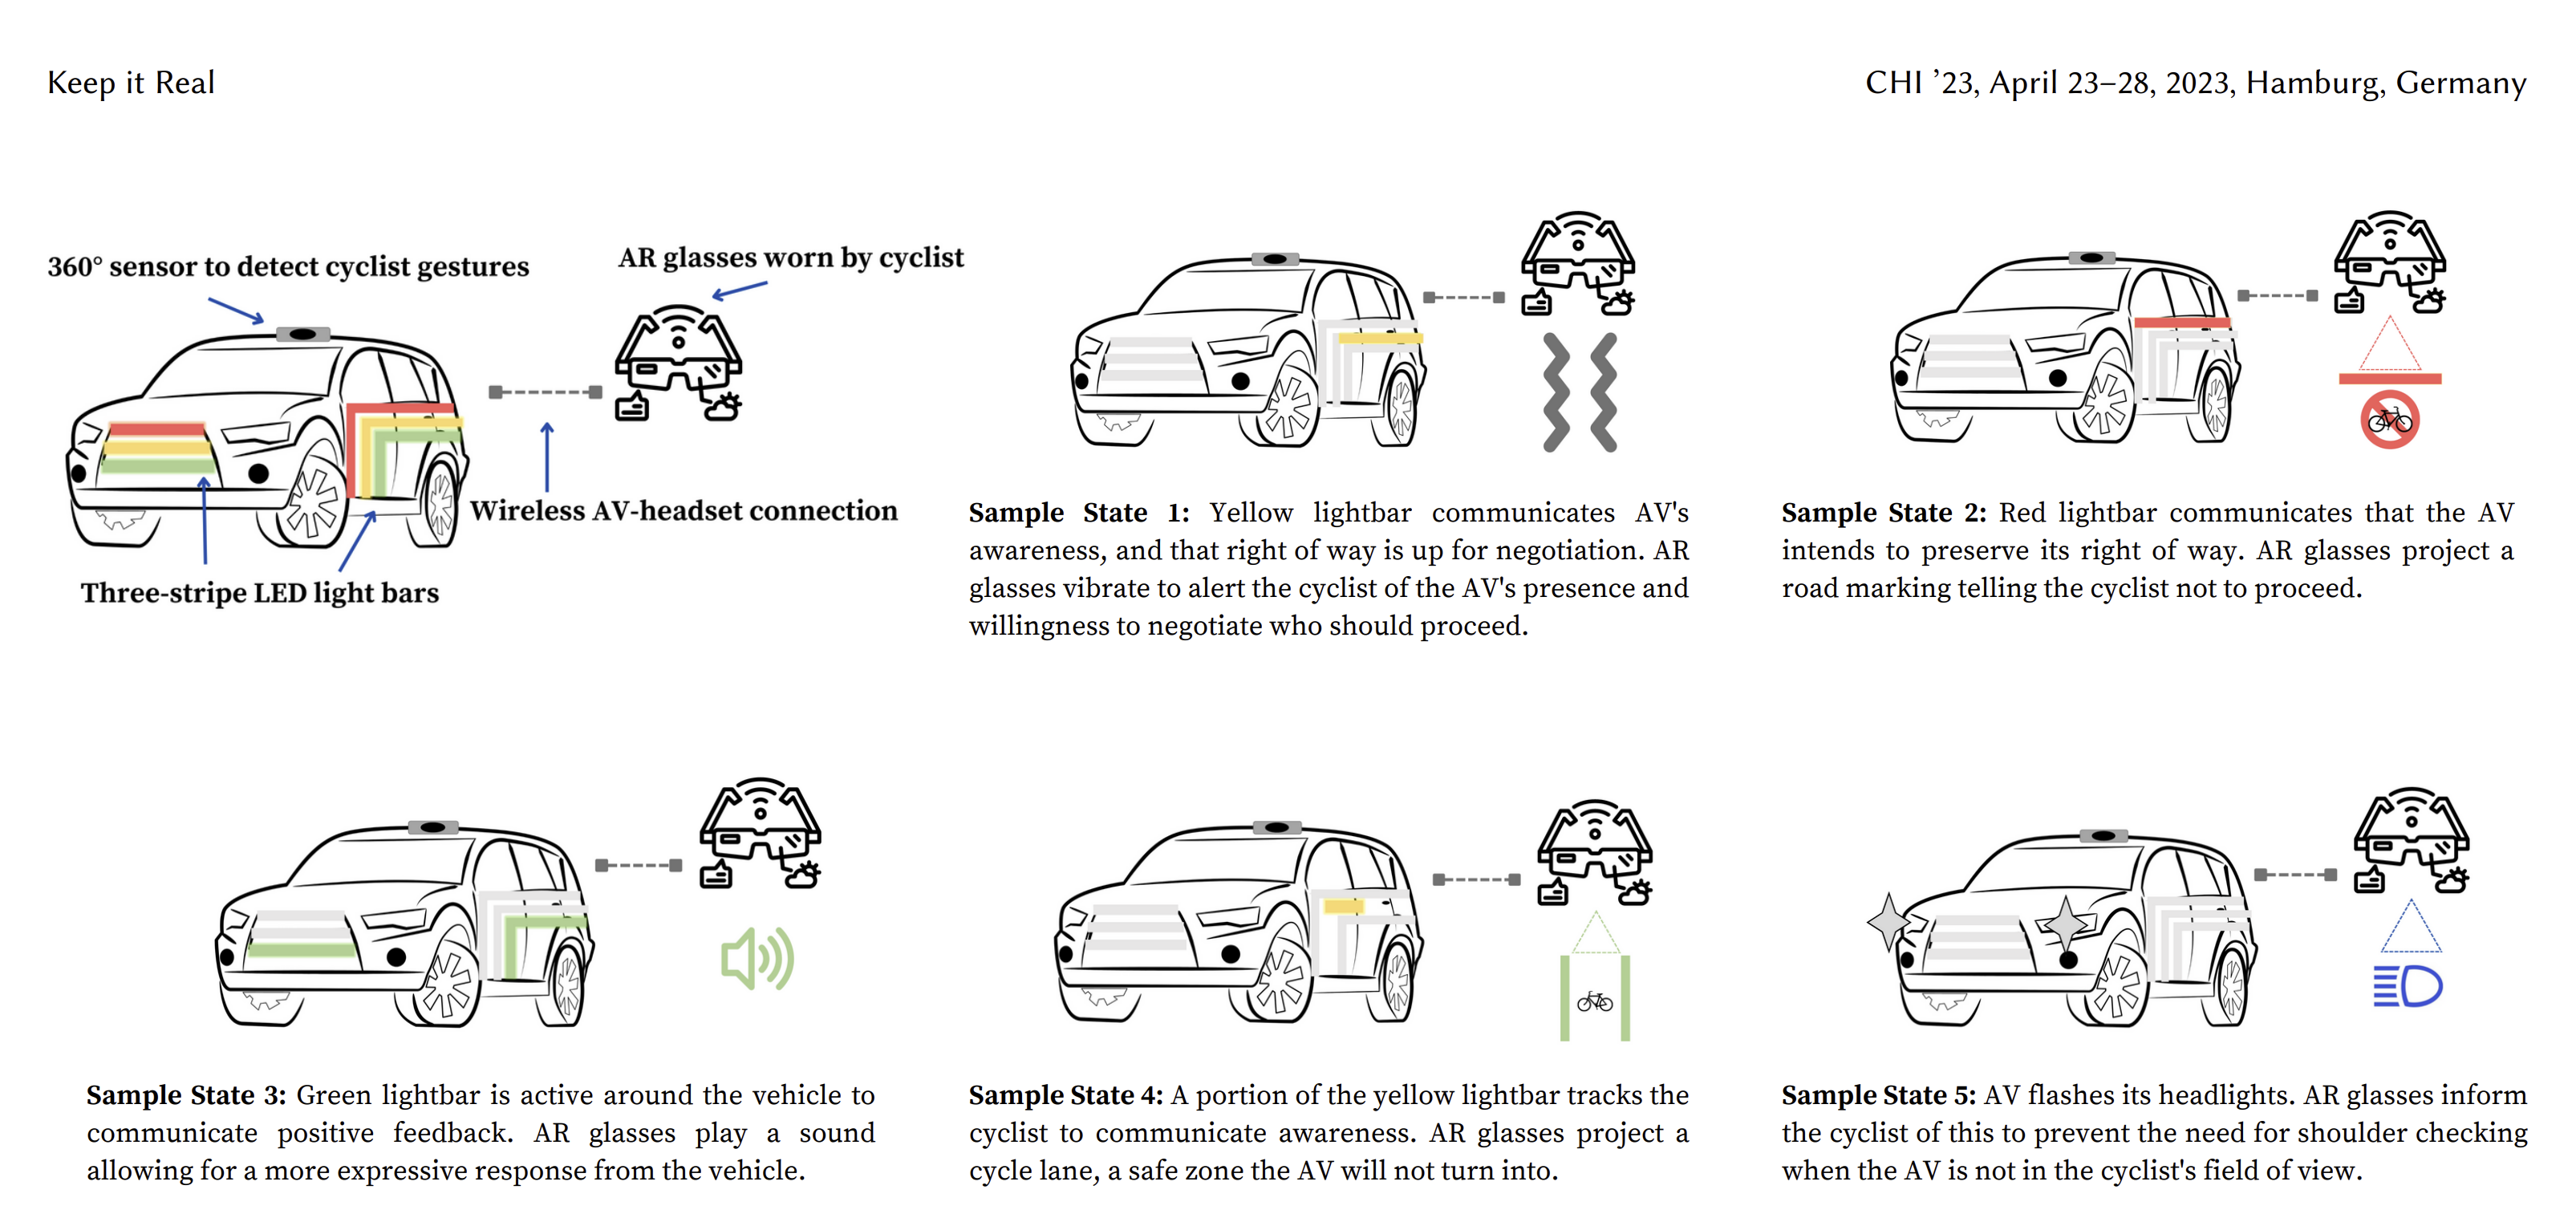
\includegraphics[width=14cm]{images/keep_it_real.png}
    \caption{The 'Keep it Real' interaction design suggestion \citep{keep_it_real}.}
    \label{fig:keep_it_real}
\end{figure}

As part of the 'Keep it Real' \citep{keep_it_real} research study, results received consisted of the distribution of cyclists gaze on vehicles when out riding on public roads. The study found that cyclists gaze mainly focused on the side and the rear of vehicles when interacting with them out on the road. As well as conducting research into gaze, the study also gives a suggestion of an interaction technique using distinct 'L' shaped LED light bars on the side of vehicles. The design suggestion given can be seen in Figure \ref{fig:keep_it_real}. In the design the lights on the side of the car show various different colours, for the prototype, I am only interested in the red, amber and green signals. The lights show red when it is not safe for the cyclist to proceed as the autonomous vehicle intends to preserve its right of way. The lights show amber when cyclists should be cautious as the right of way is up for negotiation. Finally, the lights show green when it is fine for the cyclist to proceed as they have the right of way. For the design of the graphical overlays in my prototype, I took influence from the suggestions in the study and made slight modifications to them in order to get feedback on a wider range of interaction designs. The overlays in my project were split into two different sections, side view overlays and rear view overlays.

For the side view overlays, I decided to stick with the 'L' shaped design suggested in the study. The 'L' shape design allows for coverage of the areas of high concentration of gaze, given by the results in the study. It means that no matter the situation, when a cyclist is alongside an autonomous vehicle, the design ensures that the cyclist can always see and interpret the vehicles intention and awareness of the cyclist. Similarly, I decided to stick with the traffic light colour usage, primarily due to its usage in public roads all over the world, I felt as though it would be more recognisable, easier to understand and interpret for the cyclists.

To create the application for the augmented reality headset, there are several different editors available depending on the headset and the software required, however I decided to choose Unity. Unity was chosen as it is incredibly easy to deal with, has scalability for almost any augmented reality headset and is well documented online, should I run into any errors.

\subsection{Side Design 1}

With Unity as my chosen editor, I created the first of two designs for the side view of the autonomous vehicle. The design can be seen in Figure \ref{fig:side_design1.1}, \ref{fig:side_design1.2} and \ref{fig:side_design1.3}, and follows the design recommended in the 'Keep It Real' study. The red design will be displayed to cyclists when the autonomous vehicle has seen the cyclist but has chosen to preserve its right of way. The amber design will be displayed when the autonomous vehicle has seen the cyclist and the right of way is up for negotiation. Finally, the green design will be displayed when the autonomous vehicle has seen the cyclist and has indicated that it intends to uphold the cyclists right of way.

\begin{figure}[H]
    \centering
    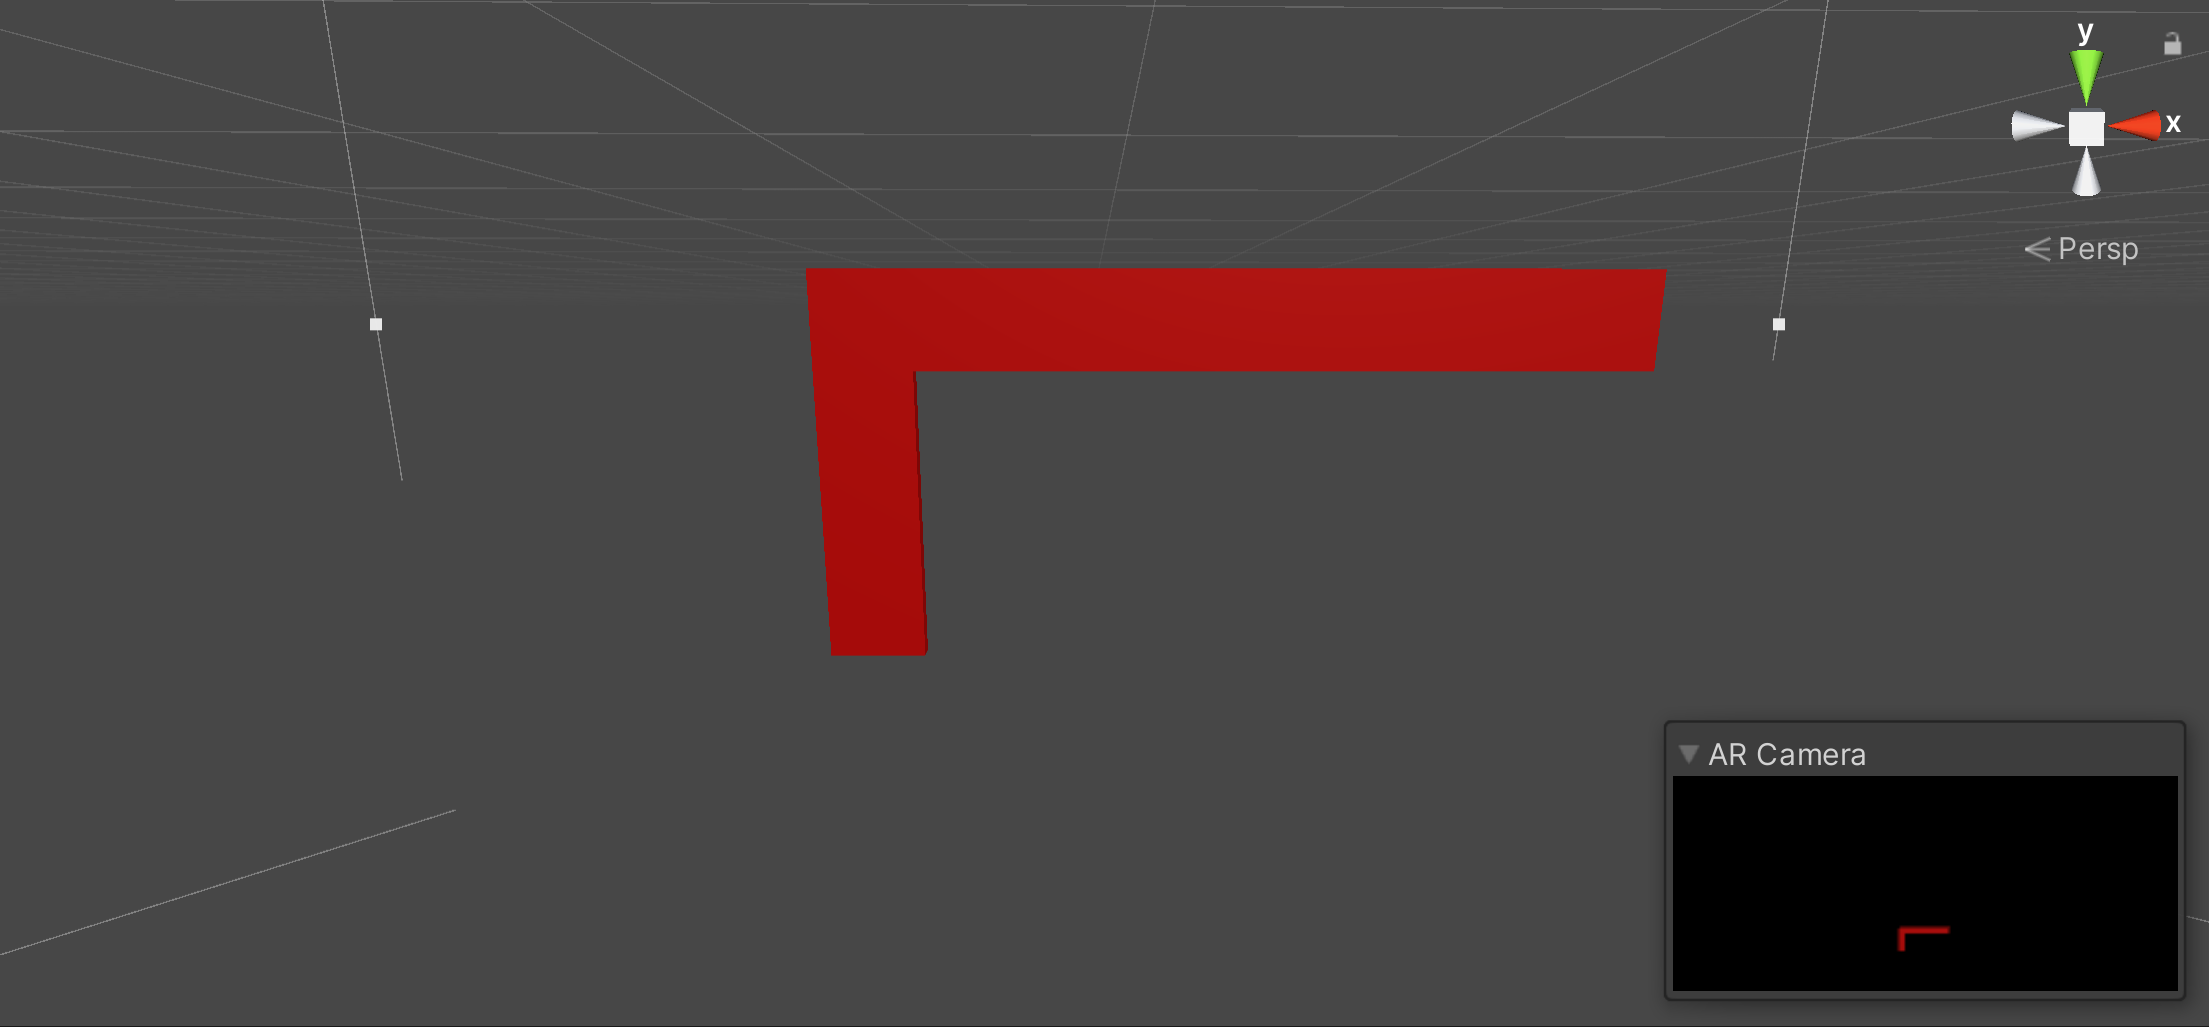
\includegraphics[width=10cm]{images/side_design1.1.png}
    \caption{Side Design 1 Red.}
    \label{fig:side_design1.1}
\end{figure}

\begin{figure}[H]
    \centering
    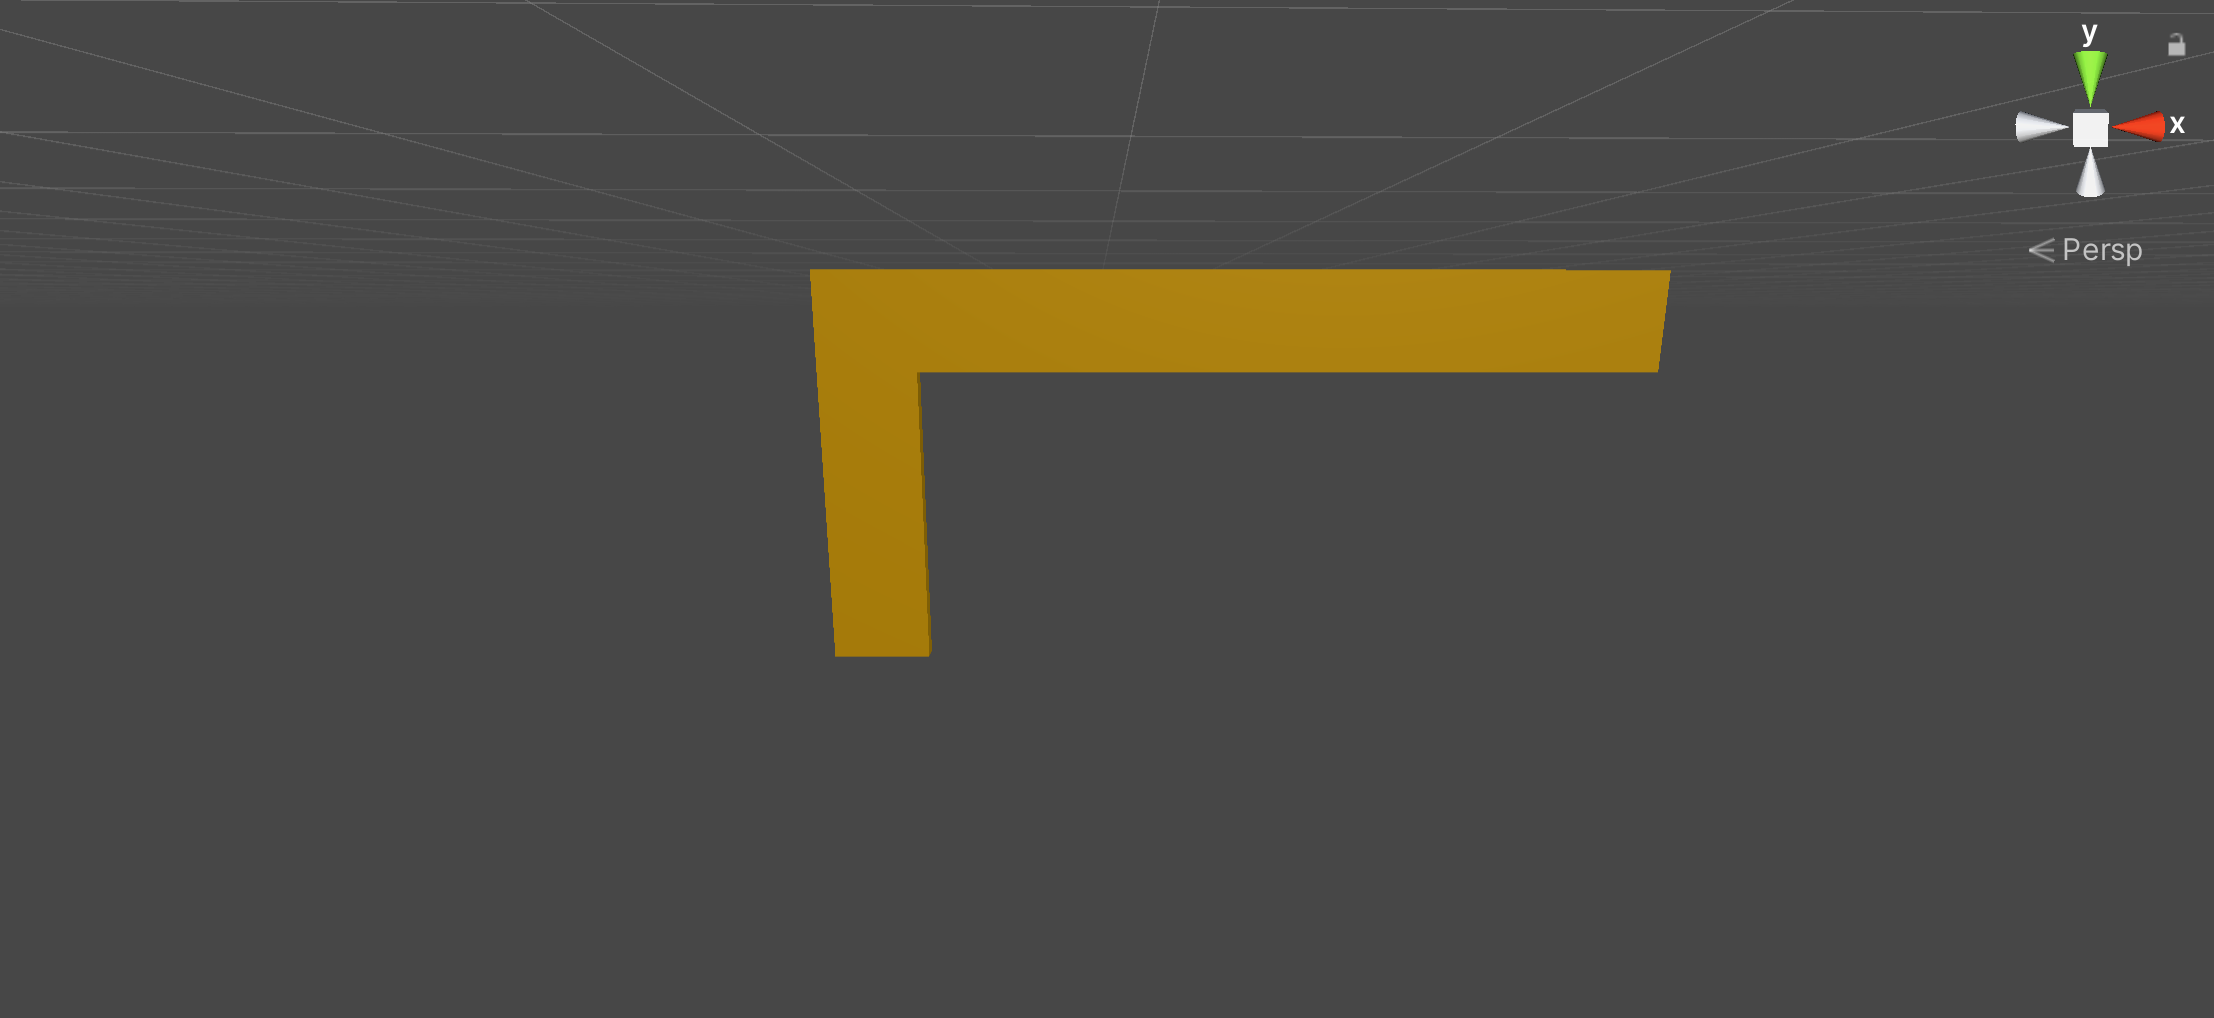
\includegraphics[width=10cm]{images/side_design1.2.png}
    \caption{Side Design 1 Amber.}
    \label{fig:side_design1.2}
\end{figure}

\begin{figure}[H]
    \centering
    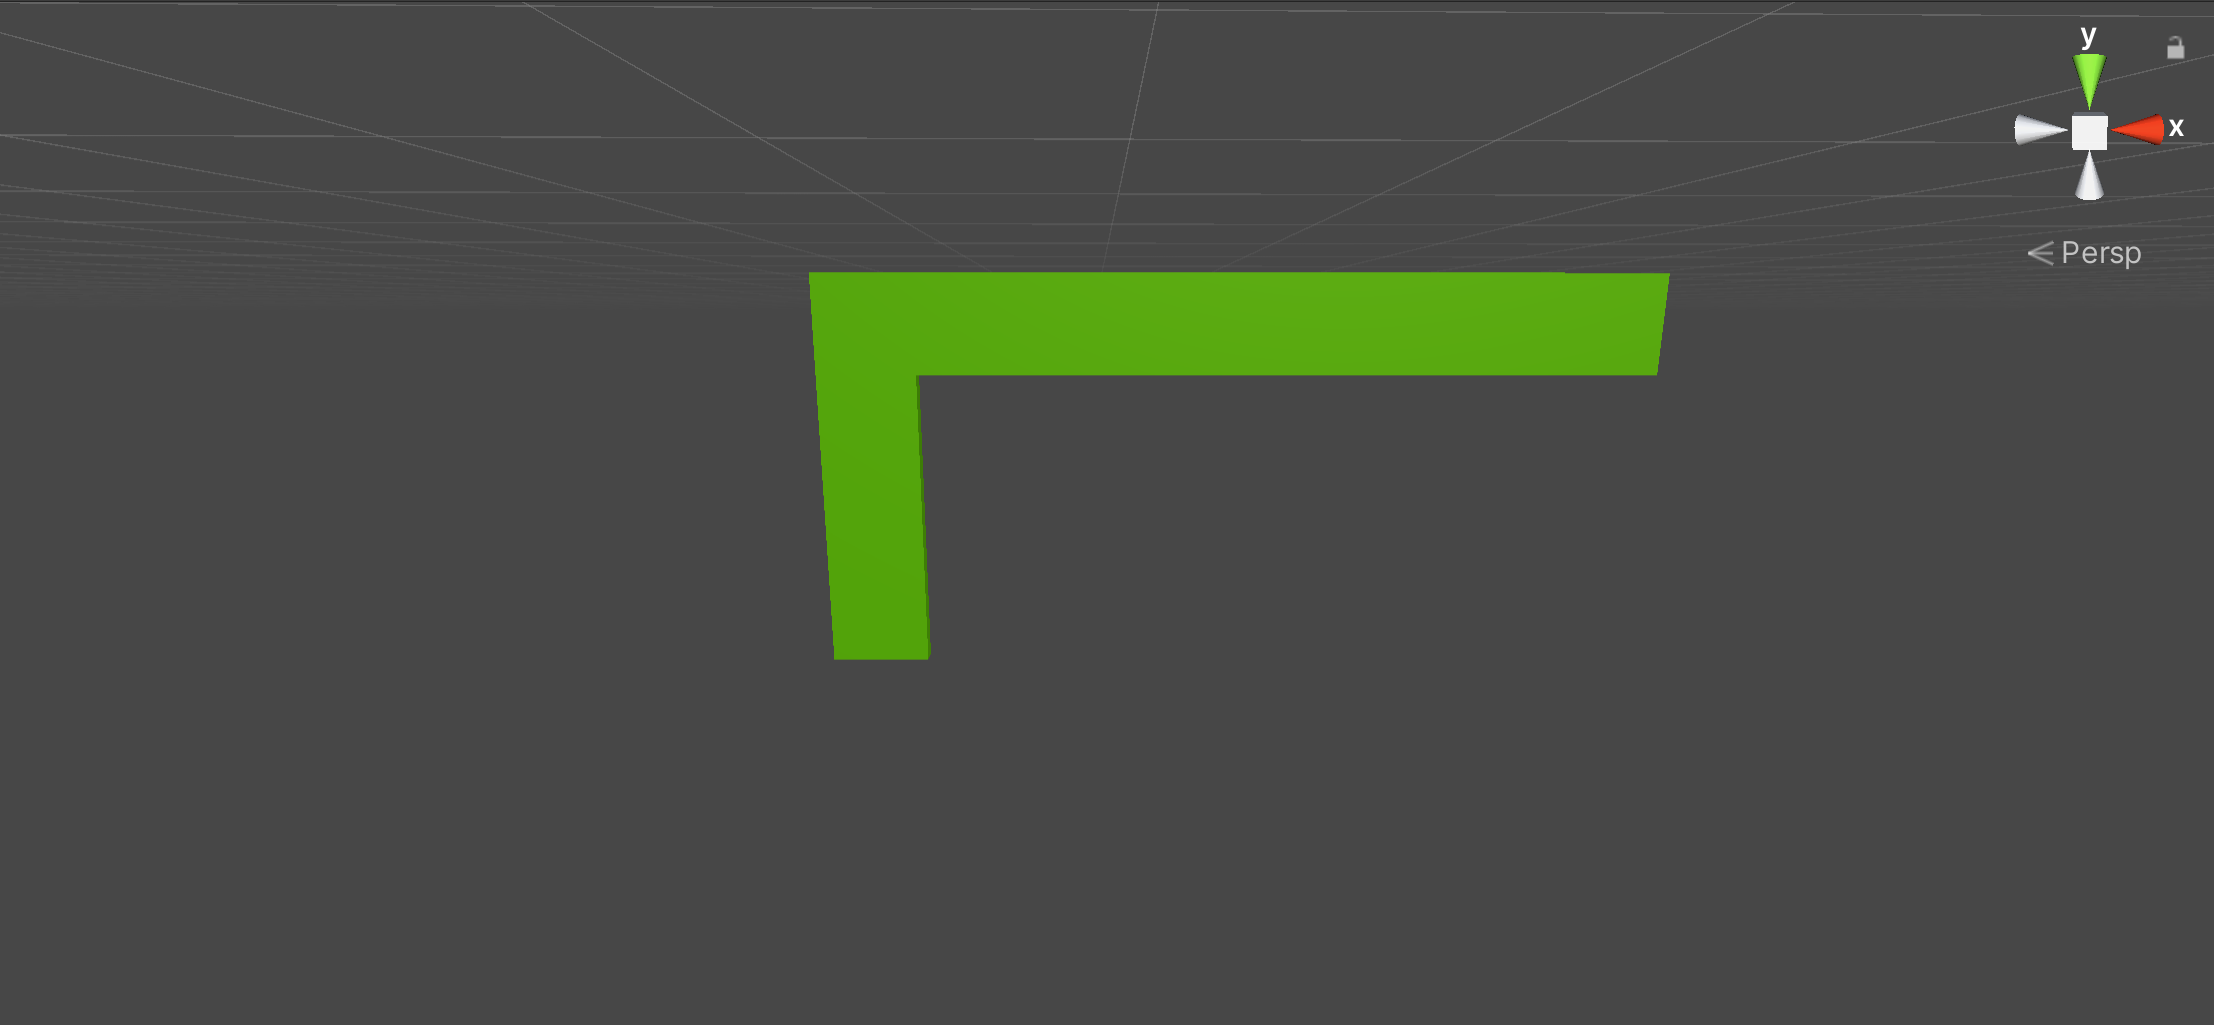
\includegraphics[width=10cm]{images/side_design1.3.png}
    \caption{Side Design 1 Green.}
    \label{fig:side_design1.3}
\end{figure}

\subsection{Side Design 2}

Whilst the design conveys a message depending on the colour, cyclists themselves may have a hard time initially understanding what each of the signals mean. Therefore, I opted to create a variation of the design that would include wording to allow for a better understanding of the signals. Adding wording to the design also ensures that cyclists who are colour blind can interpret the signals. The design with wording can be seen in Figure \ref{fig:side_design2.1}, \ref{fig:side_design2.2} and \ref{fig:side_design2.3}. The wording chosen helps to get the message across to cyclists about what they should do in each situation. In the red design, where the autonomous vehicle is going to preserve its right of way, 'DO NOT PROCEED' is shown to indicate to the cyclist that they should not pass the vehicle as it is unsafe. In the amber design, where the right of way is up for negotiation between the cyclist and autonomous vehicle, 'CAUTION' is shown to inform the cyclist that they should use caution when approaching the vehicle. In the green design, where the autonomous vehicle is going to give the cyclist the right of way, 'PROCEED' is displayed to indicate to the cyclist that they can safely approach and pass the vehicle.

\begin{figure}[H]
    \centering
    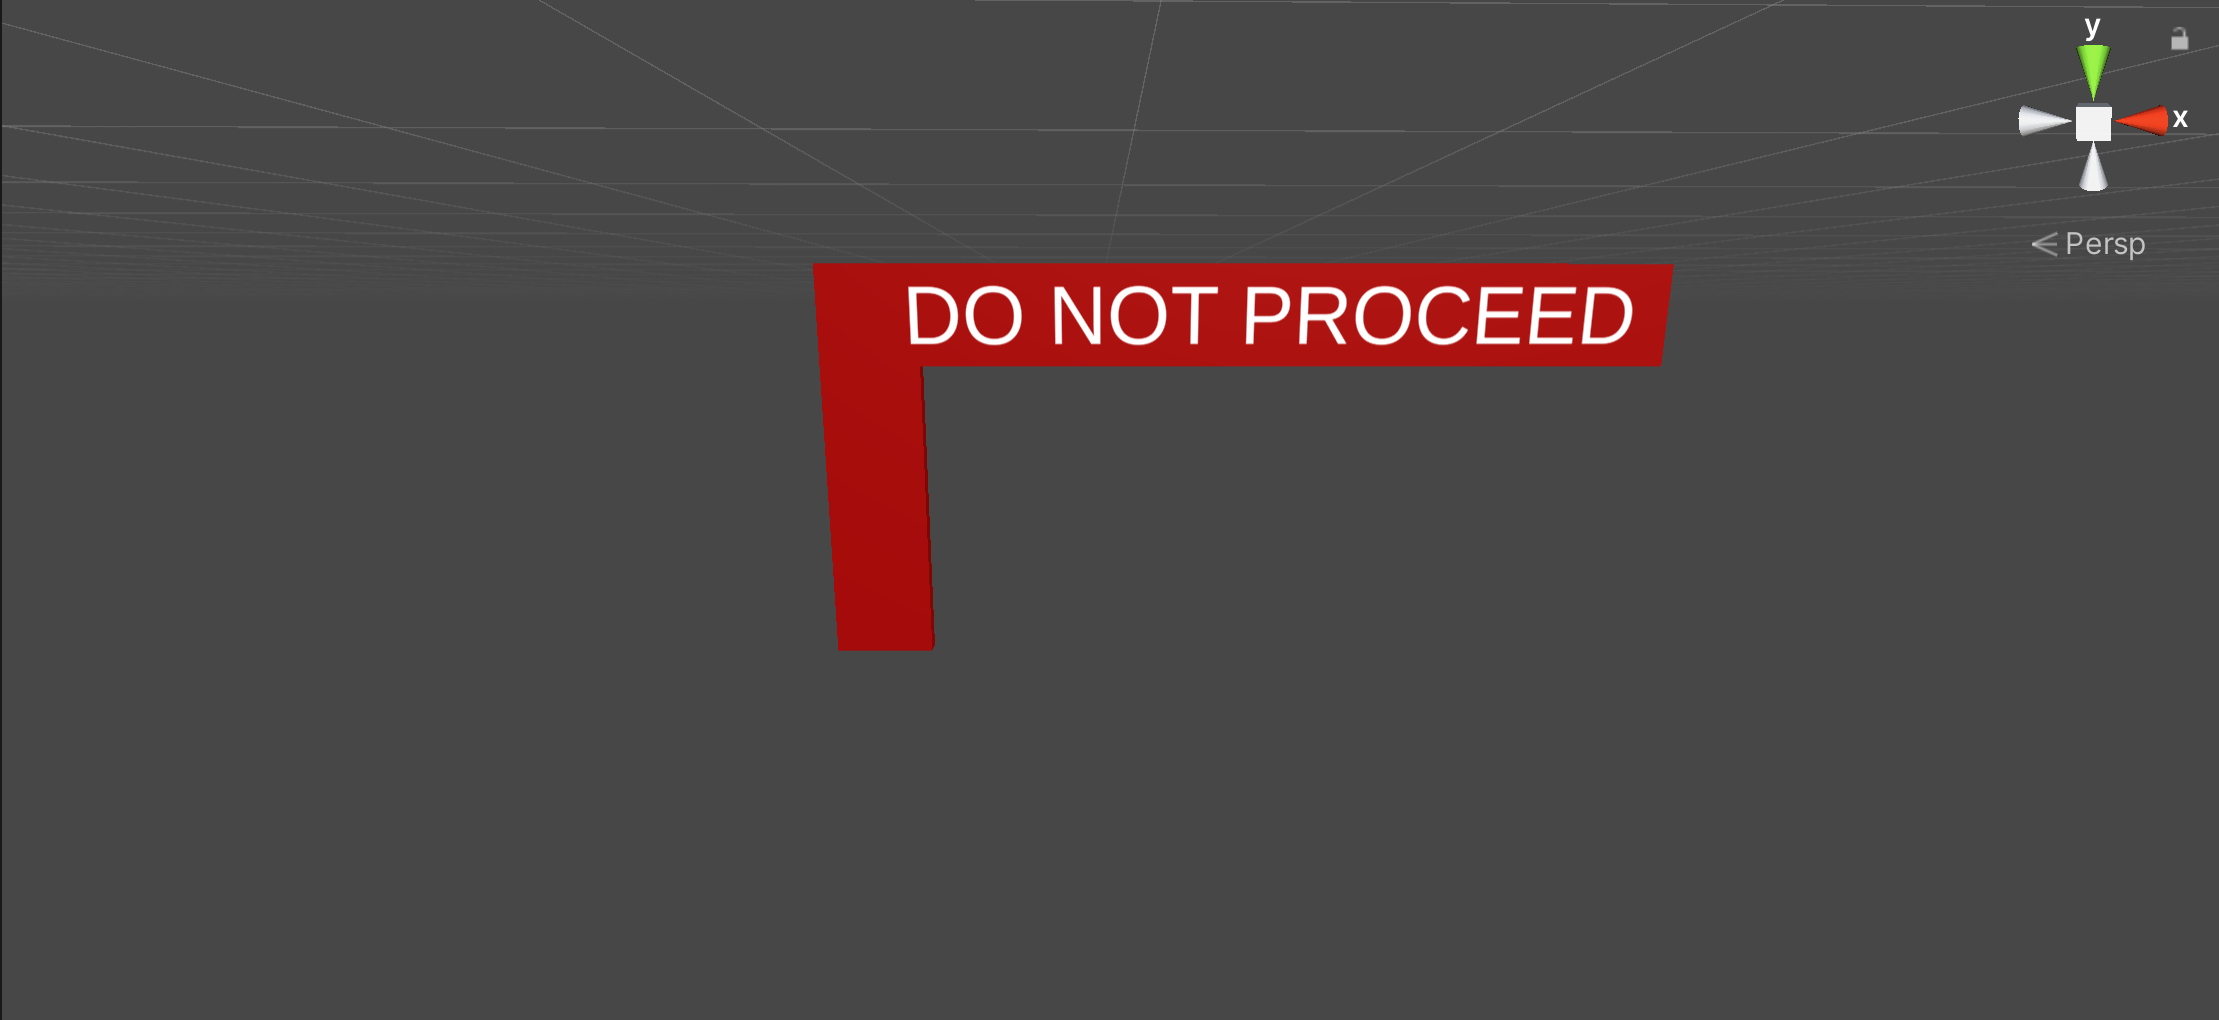
\includegraphics[width=10cm]{images/side_design2.1.png}
    \caption{Side Design 2 Red.}
    \label{fig:side_design2.1}
\end{figure}

\begin{figure}[H]
    \centering
    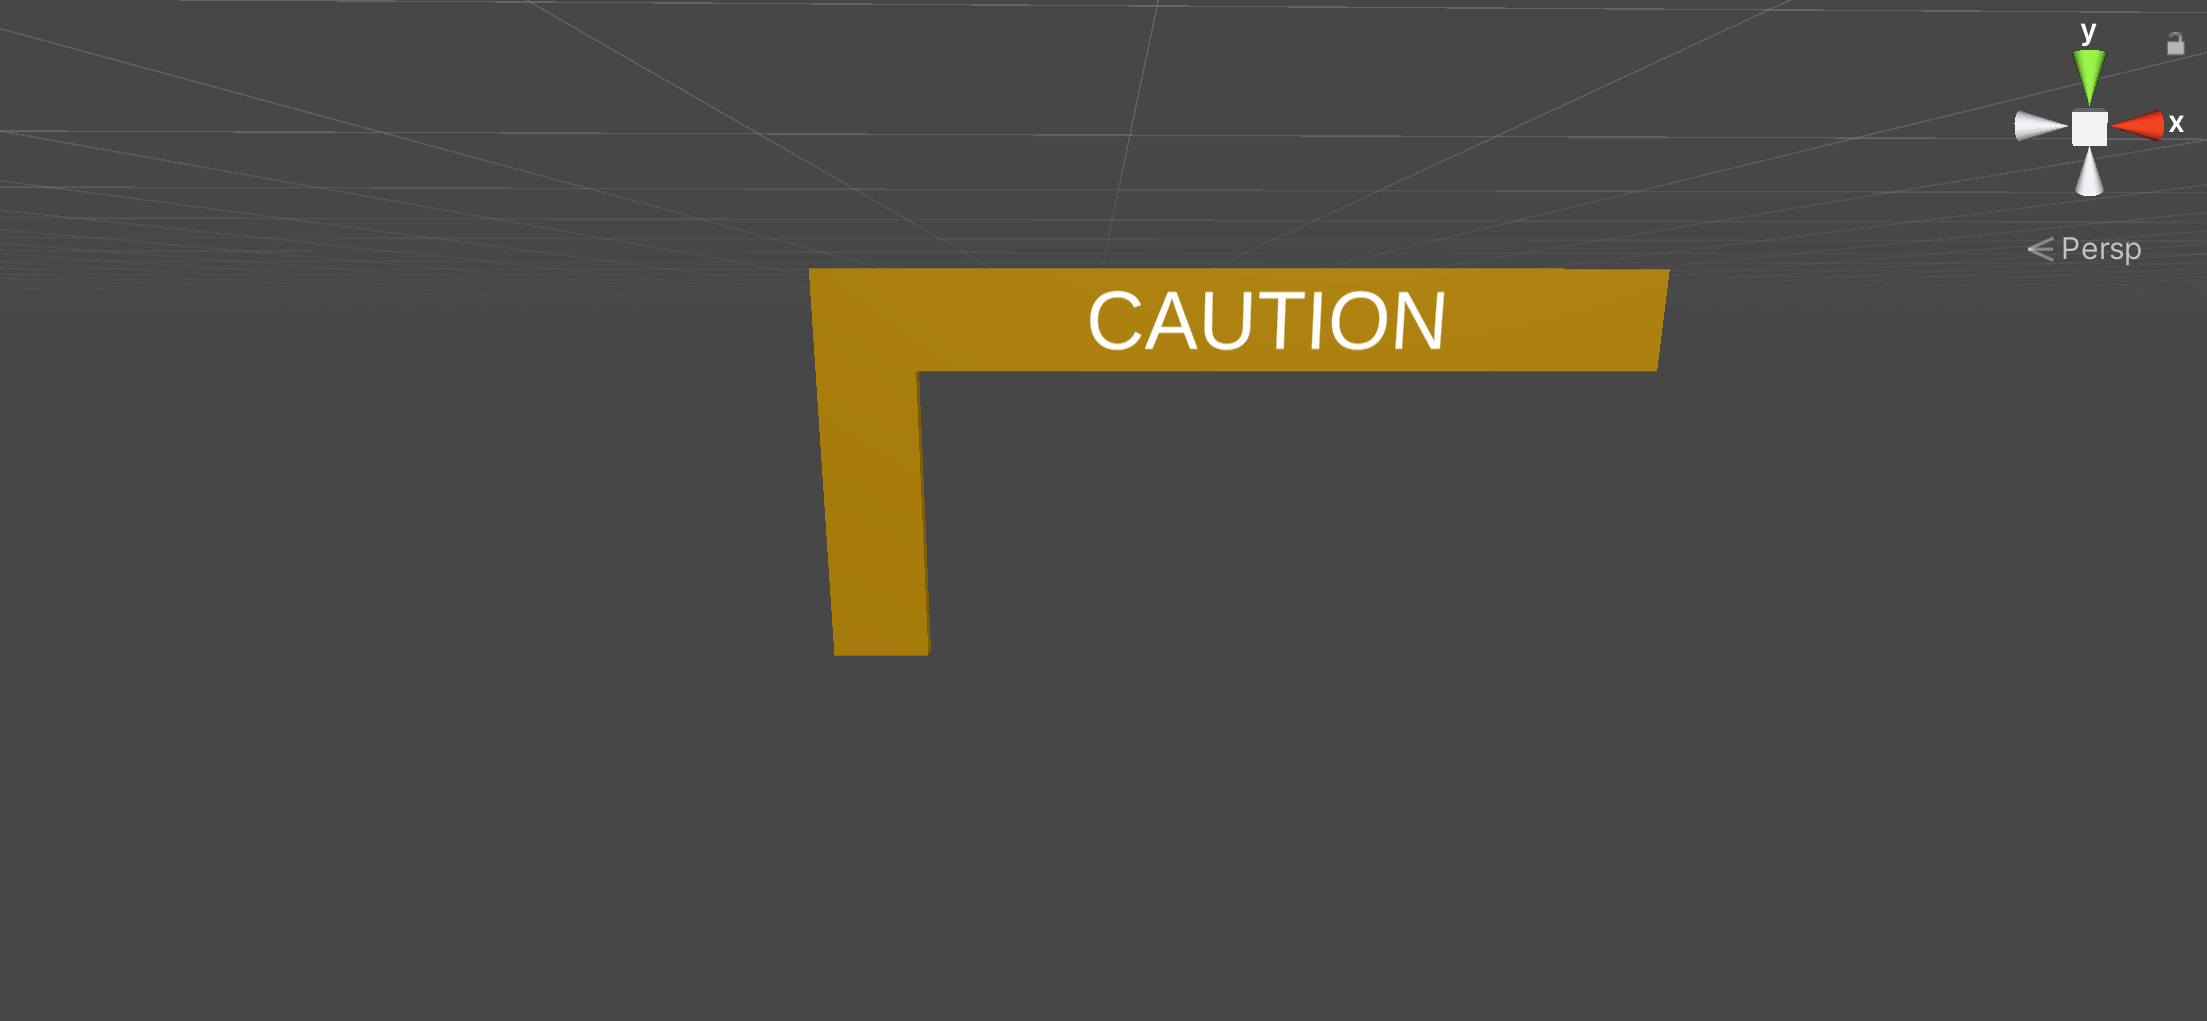
\includegraphics[width=10cm]{images/side_design2.2.png}
    \caption{Side Design 2 Amber.}
    \label{fig:side_design2.2}
\end{figure}

\begin{figure}[H]
    \centering
    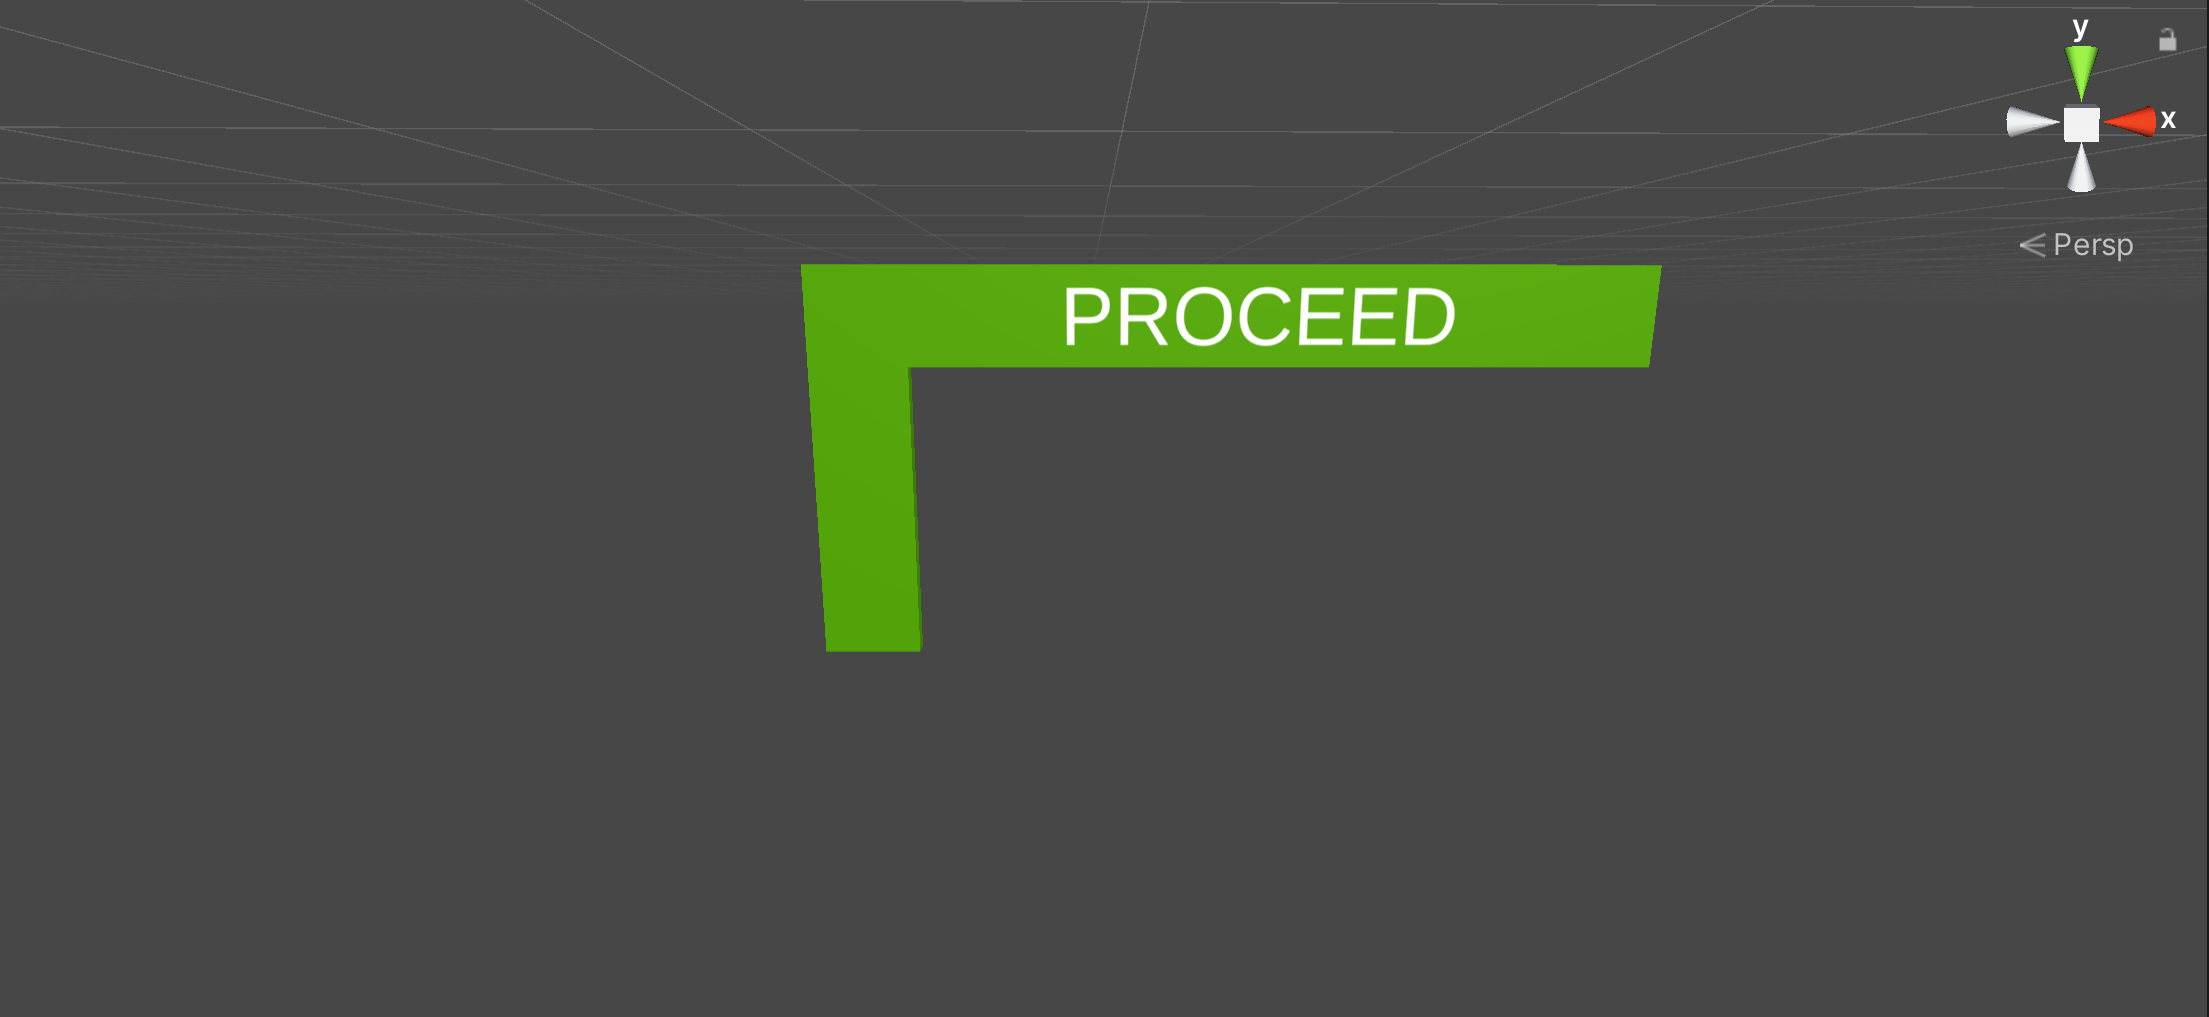
\includegraphics[width=10cm]{images/side_design2.3.png}
    \caption{Side Design 2 Green.}
    \label{fig:side_design2.3}
\end{figure}

\subsection{Rear Design 1}

Interactions between cyclists and vehicles can happen anywhere on the road. Cyclists won't always be alongside vehicles when they need to know the vehicles intention and whether they have been seen. A lot of cycling on public road is spent behind a vehicle with no way of knowing any information from the driver. This gets actively worse when there is no driver at all to provide any cues or signs to the cyclist behind them. For that reason I made the decision to create designs that would convey the intention and awareness when cyclists are behind an autonomous vehicle. This time however, instead of placing the design on the vehicle itself, the design runs parallel to the ground that the cyclist is travelling on. This means that there is less interference with the cyclists view of the vehicle and they can remain aware of the vehicles movements whilst also being shown the necessary information.

The first rear design can be seen in Figure \ref{fig:rear_design1.1}, \ref{fig:rear_design1.2} and \ref{fig:rear_design1.3}. As before, the colouring system remains the same in order to keep consistency with the other designs. The coloured plane runs along the ground just in front of the cyclist as they travel behind the vehicle, allowing for both a visual on the vehicle and on the graphical overlay.

\begin{figure}[H]
    \centering
    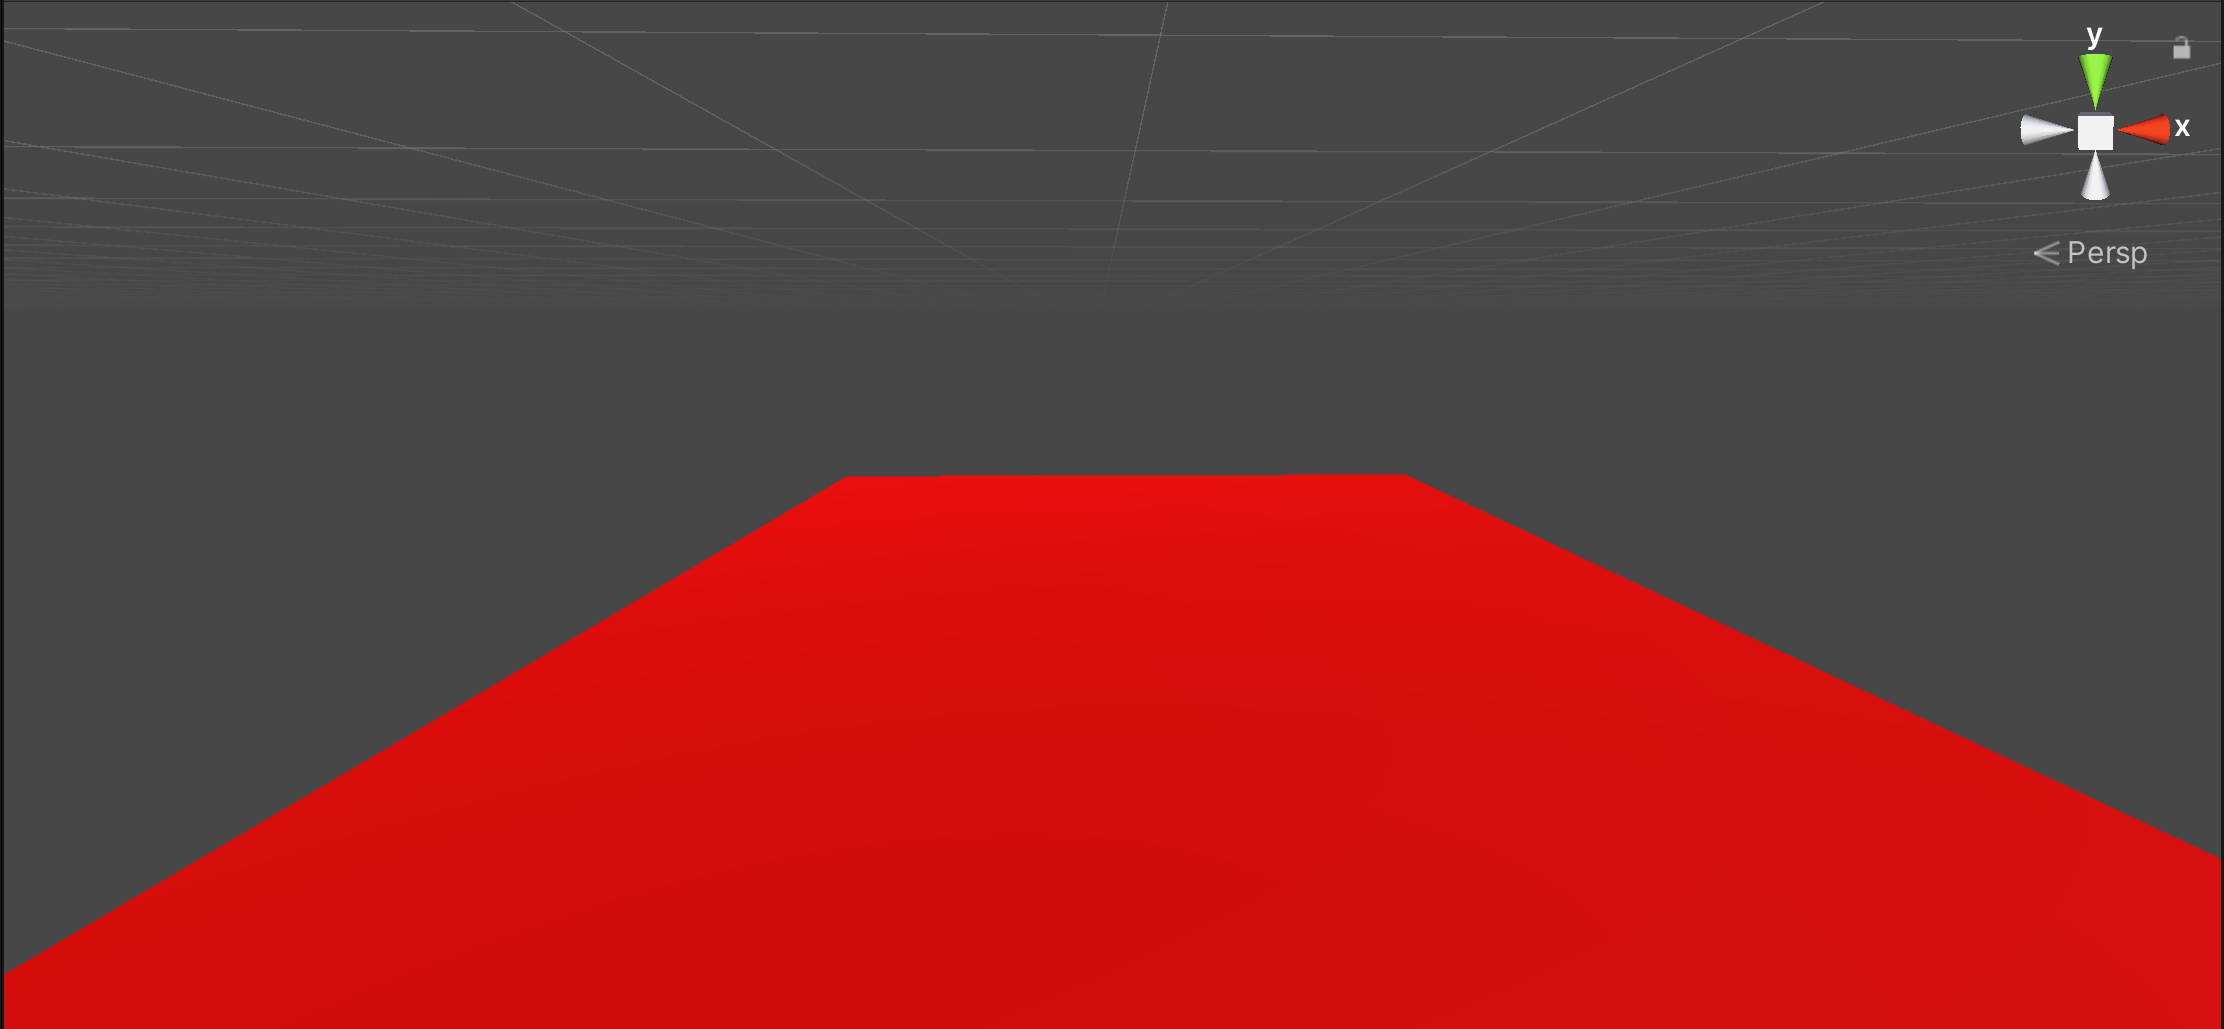
\includegraphics[width=10cm]{images/rear_design1.1.png}
    \caption{Rear Design 1 Red.}
    \label{fig:rear_design1.1}
\end{figure}

\begin{figure}[H]
    \centering
    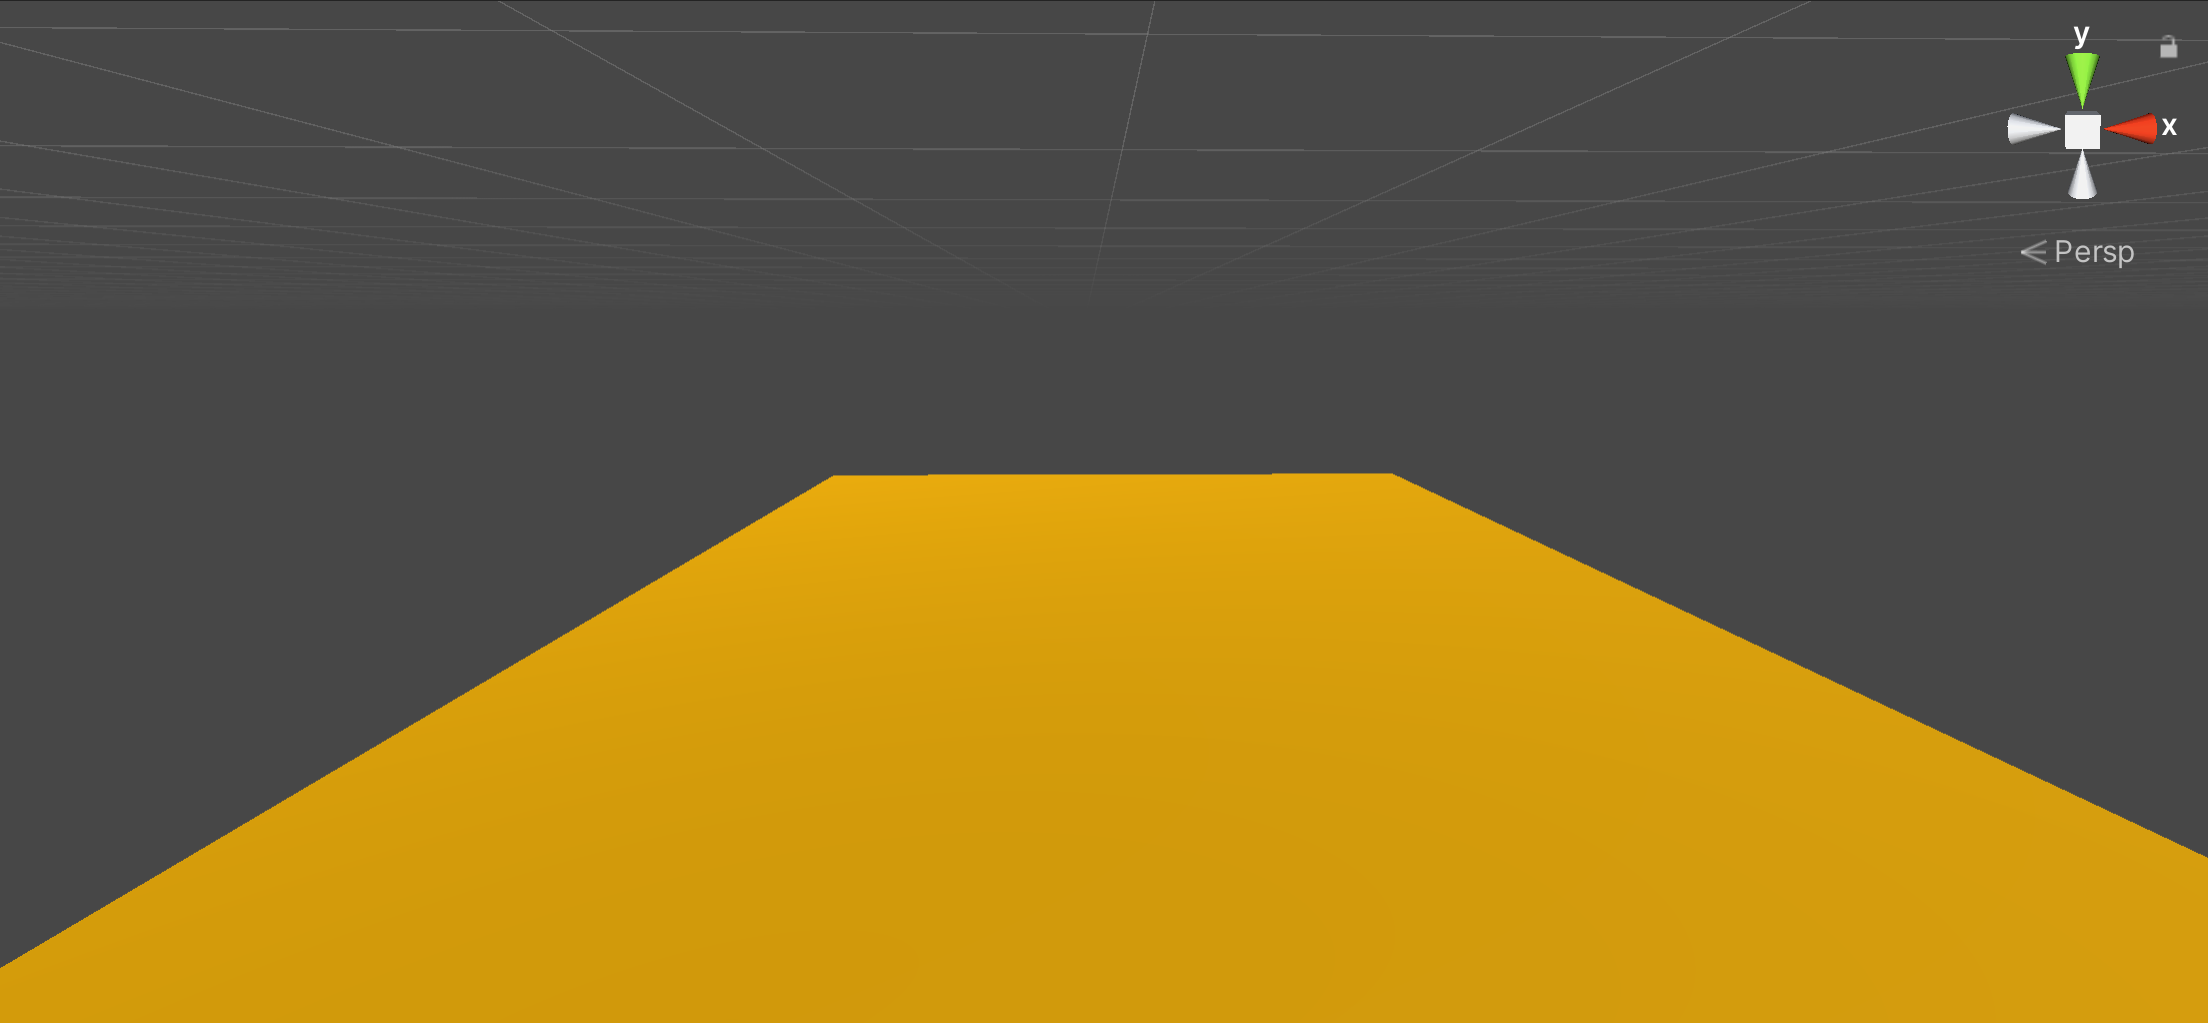
\includegraphics[width=10cm]{images/rear_design1.2.png}
    \caption{Rear Design 1 Amber.}
    \label{fig:rear_design1.2}
\end{figure}

\begin{figure}[H]
    \centering
    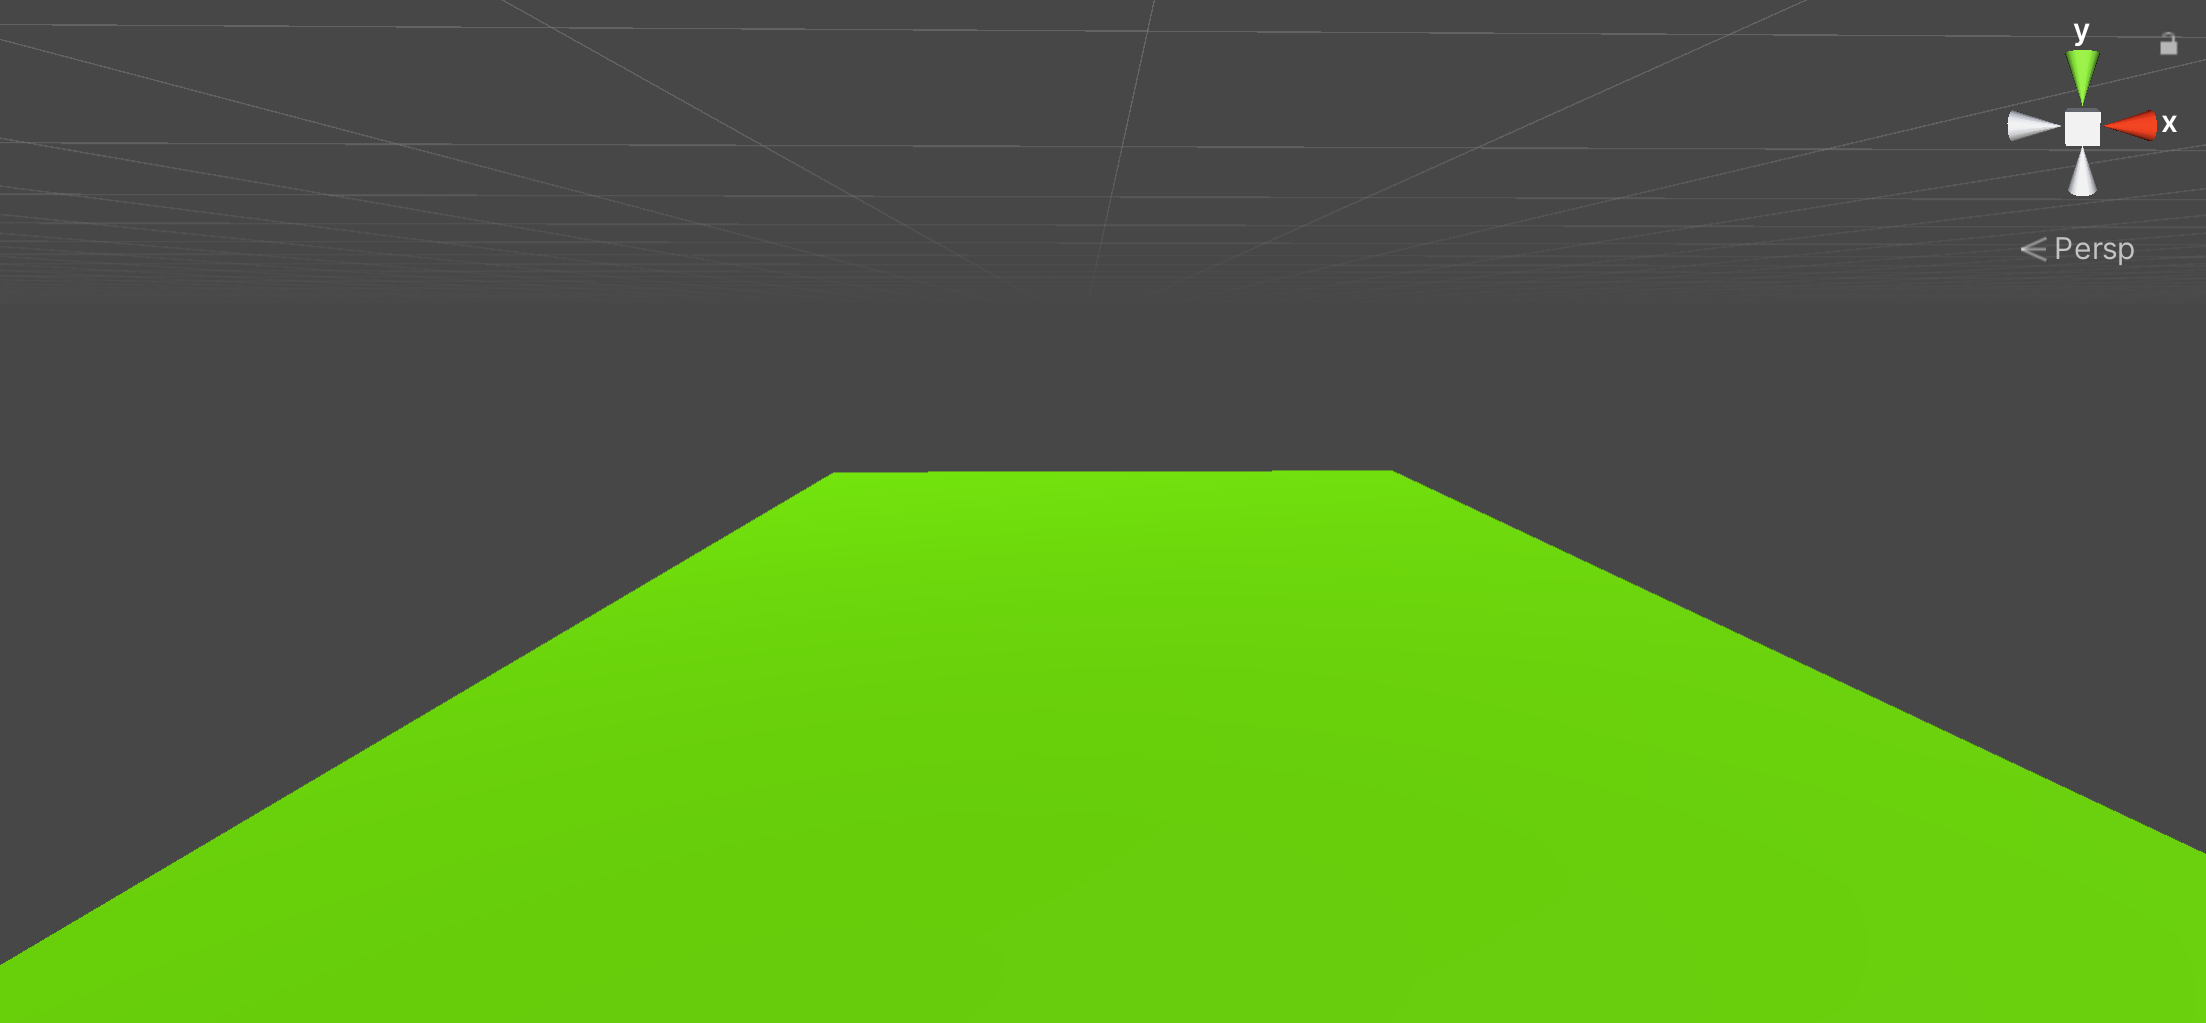
\includegraphics[width=10cm]{images/rear_design1.3.png}
    \caption{Rear Design 1 Green.}
    \label{fig:rear_design1.3}
\end{figure}

\subsection{Rear Design 2}

In a similar vein to the second side view design, to increase the accessibility and ease of understanding, I designed a variation of the rear view design that contains wording. The coloured plane still runs along the ground in front of the cyclist, only this time the design displays wording along the plane. The wording used is the same as the second side view design, 'DO NOT PROCEED' for red, 'CAUTION' for amber and 'PROCEED' for green. This design can be seen in Figure \ref{fig:rear_design2.1}, \ref{fig:rear_design2.2} and \ref{fig:rear_design2.3}.

\begin{figure}[H]
    \centering
    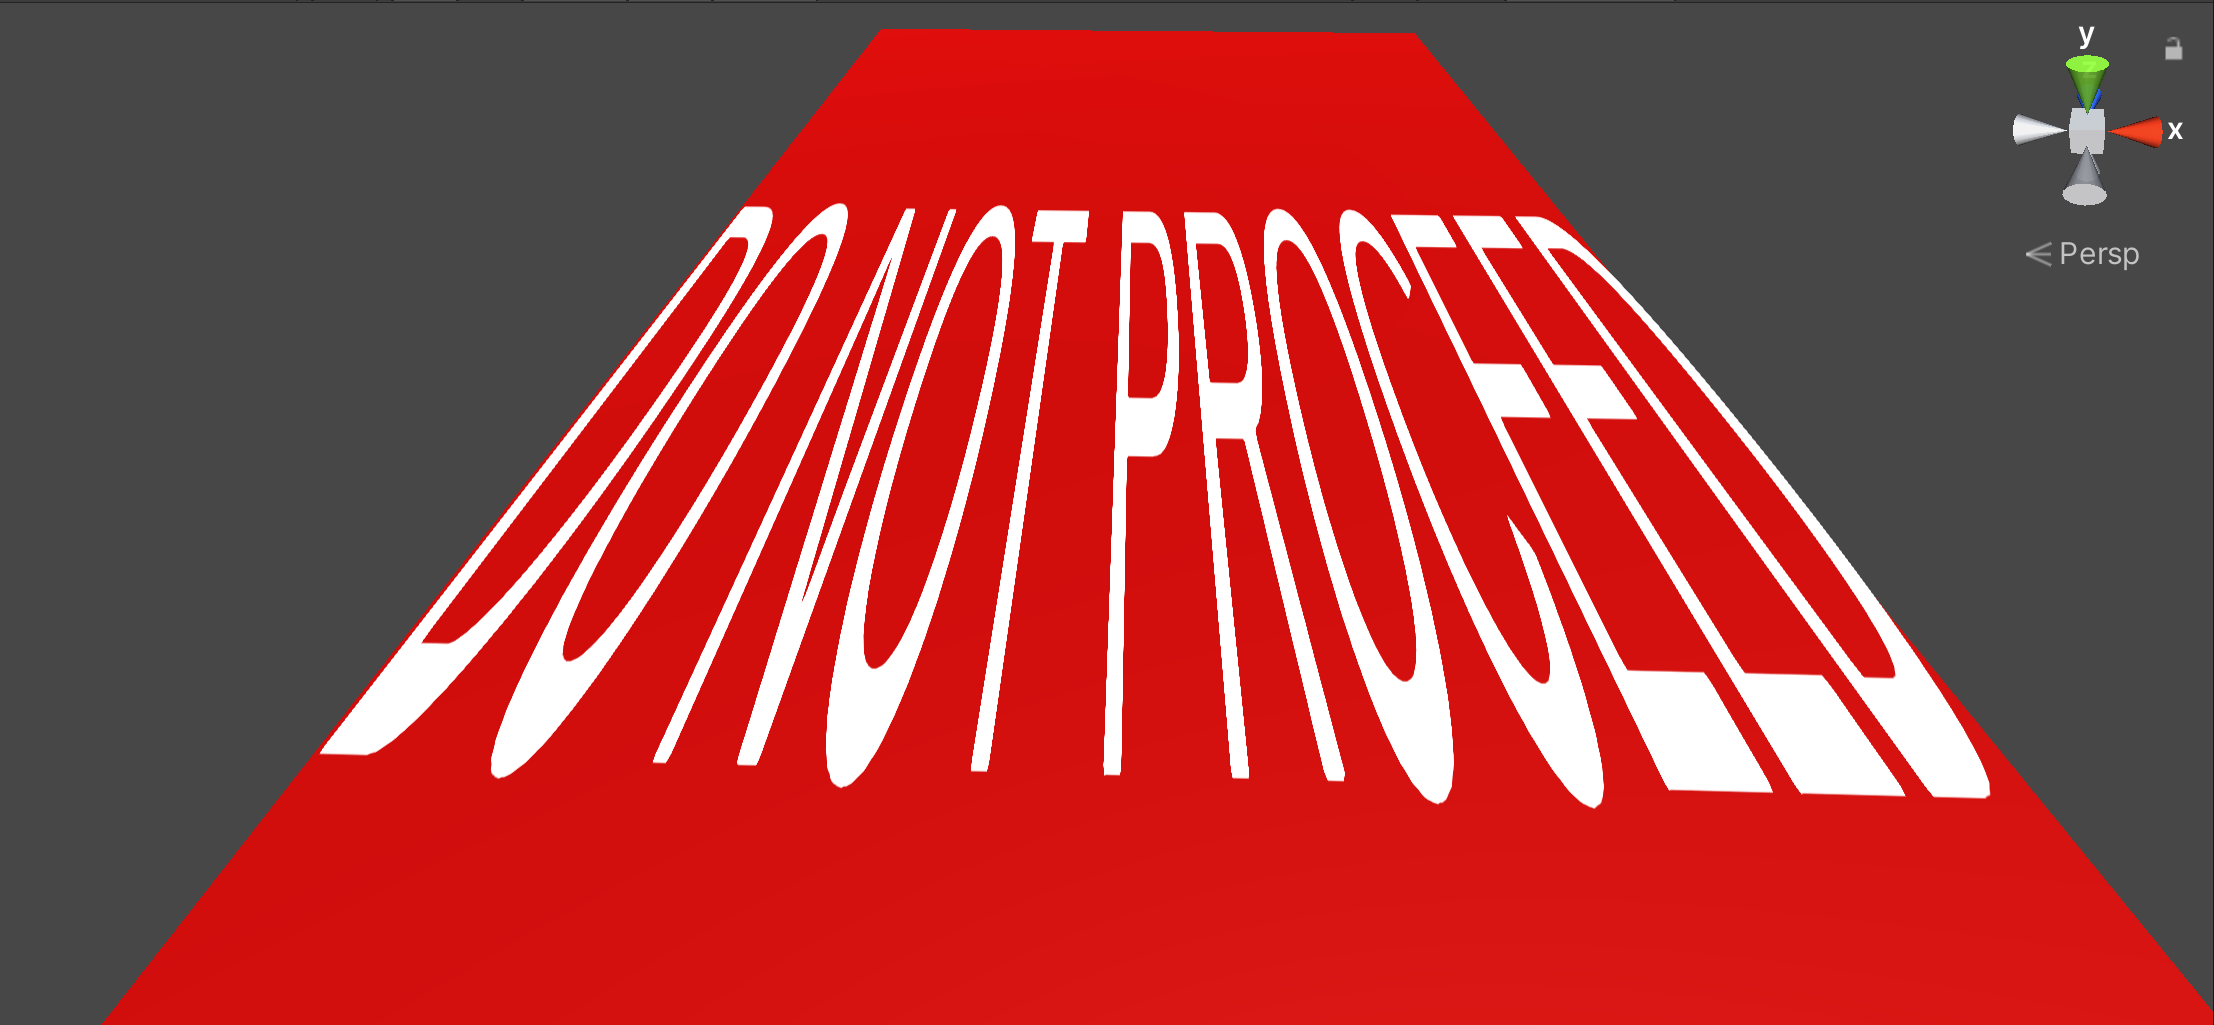
\includegraphics[width=10cm]{images/rear_design2.1.png}
    \caption{Rear Design 2 Red.}
    \label{fig:rear_design2.1}
\end{figure}

\begin{figure}[H]
    \centering
    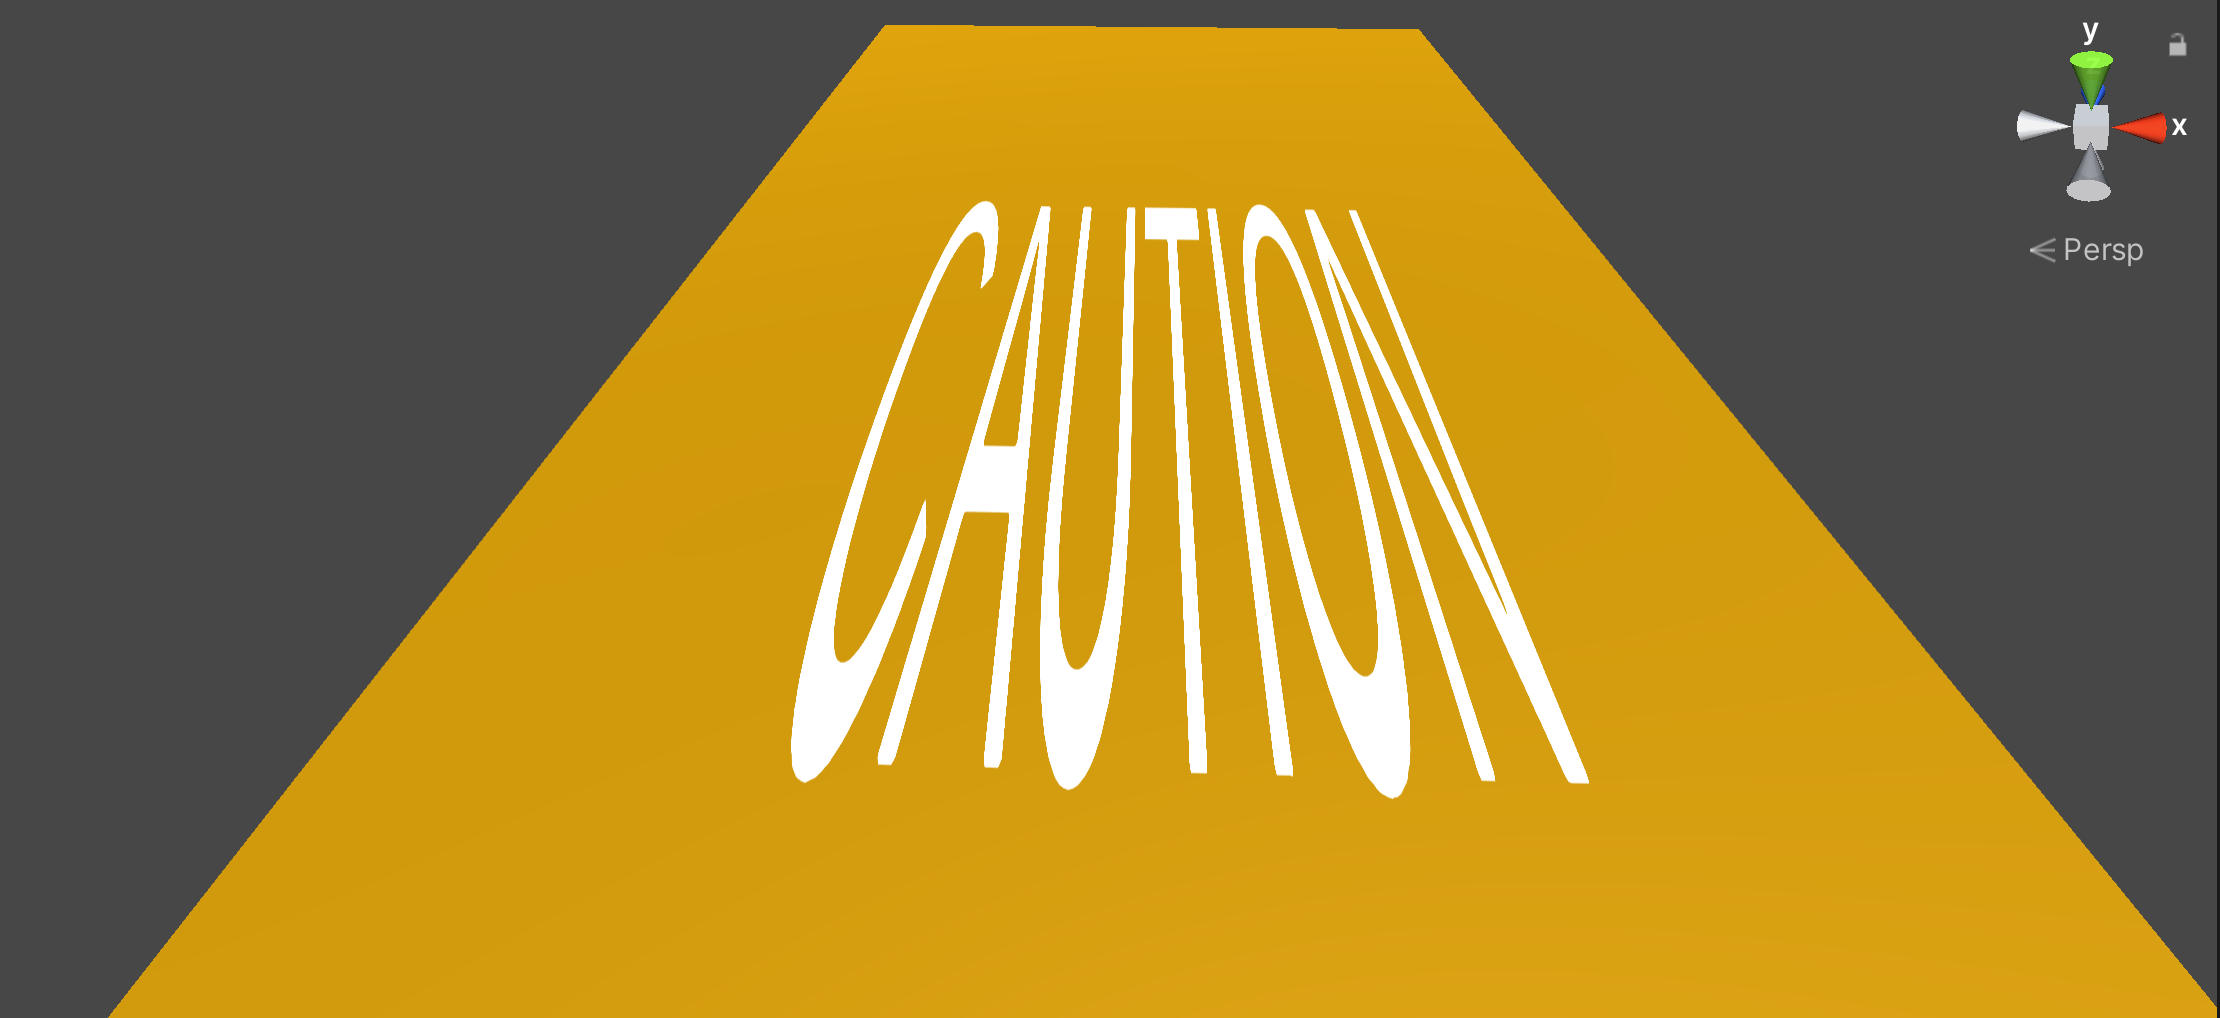
\includegraphics[width=10cm]{images/rear_design2.2.png}
    \caption{Rear Design 2 Amber.}
    \label{fig:rear_design2.2}
\end{figure}

\begin{figure}[H]
    \centering
    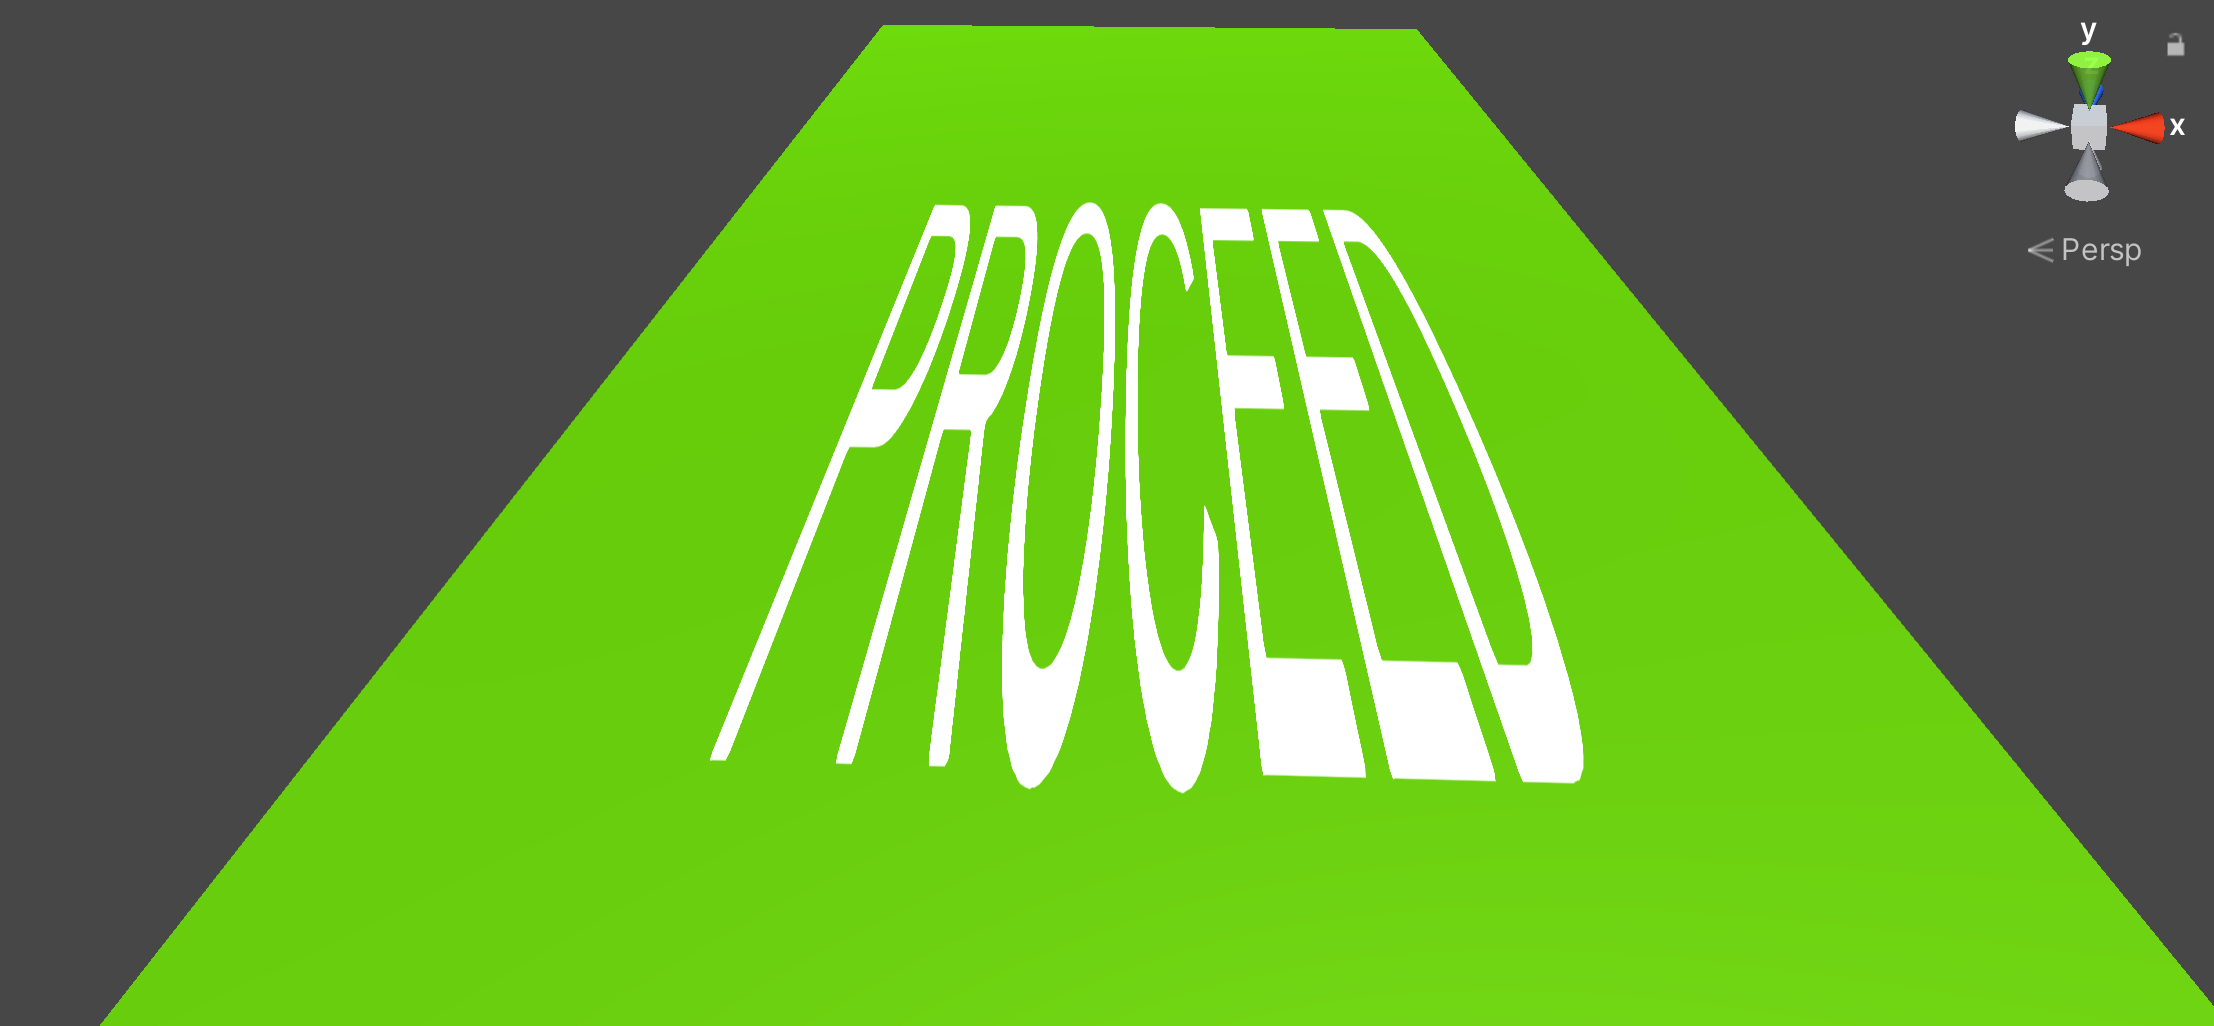
\includegraphics[width=10cm]{images/rear_design2.3.png}
    \caption{Rear Design 2 Green.}
    \label{fig:rear_design2.3}
\end{figure}

%==================================================================================================================================

\chapter{Implementation}

\section{Vehicle Detection}

\subsection{You Only Look Once}

Initially You Only Look Once, YOLO, was intended for the vehicle detection aspect of the project. As mentioned earlier, YOLO is a single-stage network object detection algorithm created by Joseph Redmon and Ali Farhadi in 2015. The algorithm partitions the inputted image into a grid of cells and for each cell it predicts the probability of an object existing, the bounding box for the object and the class of the object \citep{yolo}. YOLO processes the entire image in only one pass which makes it faster and more efficient than other object detection algorithms, which is ideal for this project as we require real time object detection.

Despite my best efforts, I only managed to get YOLO running using processing power. Object detection algorithms work best, and are at their most efficient, when they run on graphics processing units as the heavy work load requires a dedicated piece of hardware. Running YOLO on a processor alone yielded poor results and the object detection was nowhere near the real time speed required for this project. Unfortunately, YOLO has very specific requirements to run, including the need for an NVIDIA graphics processing unit. Whilst I had originally planned to use YOLO, so much time was spent attempting to get it to work that I eventually had to change the approach to use other object detection methods.

Regardless of the fact that it did not work out for my project, YOLO is a fantastic algorithm that will have a major impact on the future of technology. Future implementations of similar projects may benefit from YOLO having the potential to only require one device to run an entire prototype on, i.e. without the need for a local machine to run object detection on.

\subsection{Zed 2}

\begin{figure}[H]
    \centering
    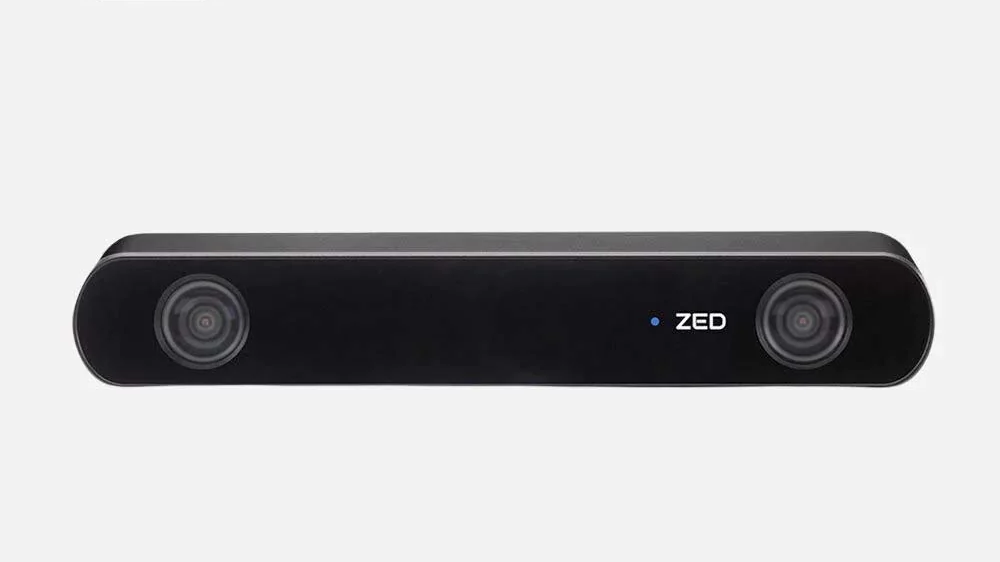
\includegraphics[width=10cm]{images/zed.png}
    \caption{Zed 2 Stereo Camera by StereoLabs \citep{zed_image}.}
    \label{fig:zed}
\end{figure}

Following the failed implementation of YOLO, there was various other methods of object detection I had to choose from. Considering the main focus of the project was human-computer interaction and not computer vision, I required an easier to implement approach that would ensure I could spend more time on the evaluation of the prototype. The decision was made to try out an external piece of hardware to manage the object detection, I was therefore loaned out a Zed 2 camera from the university.

The Zed 2 is a stereo camera that was developed by StereoLabs that has a vast array of features and potential applications. The camera itself can perform depth perception, motion tracking and spatial AI, ideal for this projects requirements, and simply requires a USB connection to a local machine to function \citep{zed_image}. Figure \ref{fig:zed} shows an image of the Zed 2 Stereo camera.

In order to start working with the Zed 2 camera, the software development kit for the camera must first be downloaded. The software development kit provides all of the software required to get the camera up and running. The Zed 2 can be ran using several different programming languages, in my case I chose the language I am most familiar with, Python. Within the software development kit is a range of different tutorials and examples which showcase the different applications of the camera. Most importantly, for this project, there is an example piece of code which performs object detection.

The base code provided creates and initialises the camera instance, contains a confidence threshold as a percentage that can be altered and then detects objects and returns information based on what the camera has seen. The information that the code returns are attributes of the detected object including the label, confidence level, tracking ID, tracking state, bounding box and most importantly a three dimensional coordinate of the object.

Several additions and edits were made to the base code to fit the needs for this project. After running several tests using the camera, I had found that using a confidence threshold of 80 percent was ideal, this was high enough to ensure that any false positives were rejected and was low enough to identify the majority of vehicles in daylight. In the main body of the object detection code, I added a 'Try/Except' statement that also used an infinite 'While' loop to allow the camera to run indefinitely until I desired. Initially the code ran for a certain number of seconds, which became a nuisance during testing and I found being able to end the program when I desired with a keyboard interrupt to be far better. Finally, this project only requires the detection of vehicles, so having the code returning information on objects that were not classed as vehicles was unnecessary and a waste of resources. To combat this, I added a simple 'If' statement which checks the label of the object detected and only allows the display of information if the label contains 'Vehicle'. The code with all of the edits can be seen in Figure \ref{lst:code1} and \ref{lst:code2}.

\begin{lstlisting}[language=python, float, caption={Python Vehicle Detection Code Part 1, Original Code Without Edits Copyright (c) 2022, STEREOLABS.}, label={lst:code1}]
import pyzed.sl as sl
import numpy as np
import struct

def main():
    # Create a Camera object
    zed = sl.Camera()

    # Create a InitParameters object and set configuration parameters
    init_params = sl.InitParameters()
    init_params.depth_mode = sl.DEPTH_MODE.PERFORMANCE
    init_params.coordinate_units = sl.UNIT.METER
    init_params.sdk_verbose = 1

    # Open the camera
    err = zed.open(init_params)
    if err != sl.ERROR_CODE.SUCCESS:
        print("Camera Open : "+repr(err)+". Exit program.")
        exit()

    obj_param = sl.ObjectDetectionParameters()
    obj_param.enable_tracking=True
    obj_param.enable_segmentation=True
    obj_param.detection_model = sl.OBJECT_DETECTION_MODEL.MULTI_CLASS_BOX_MEDIUM

    if obj_param.enable_tracking :
        positional_tracking_param = sl.PositionalTrackingParameters()
        #positional_tracking_param.set_as_static = True
        zed.enable_positional_tracking(positional_tracking_param)

    print("Object Detection: Loading Module...")

    err = zed.enable_object_detection(obj_param)
    if err != sl.ERROR_CODE.SUCCESS :
        print("Enable object detection : "+repr(err)+". Exit program.")
        zed.close()
        exit()

    objects = sl.Objects()
    obj_runtime_param = sl.ObjectDetectionRuntimeParameters()
    # I changed threshold to 80% confidence.
    obj_runtime_param.detection_confidence_threshold = 80
\end{lstlisting}

\begin{lstlisting}[language=python, float, caption={Python Vehicle Detection Code Part 2, Original Code Without Edits Copyright (c) 2022, STEREOLABS.}, label={lst:code2}]
 # I added Try/Except with while statement and keyboard interrupt in order to allow the script to run indefinitely. 
    try:
        while True:
            zed.grab()
            zed.retrieve_objects(objects, obj_runtime_param)
            if objects.is_new :
                obj_array = objects.object_list
                print(str(len(obj_array))+" Object(s) detected\n")
                if len(obj_array) > 0 :
                    object = obj_array[0]
                    # I added If statement to remove uneccassary info from labels other 'Vehicle'.
                    if repr(object.label) == 'Vehicle':
                        print("Object attributes:")
                        print(" Label '"+repr(object.label)+"' (conf. "+str(int(object.confidence))+"/100)")
                        if obj_param.enable_tracking :
                            print(" Tracking ID: "+str(int(object.id))+" tracking state: "+repr(object.tracking_state)+" / "+repr(object.action_state))
                        velocity = object.velocity
                        dimensions = object.dimensions
                        print(" 3D position: [{0},{1},{2}]\n Velocity: [{3},{4},{5}]\n 3D dimensions: [{6},{7}{8}]".format(position[0],position[1],position[2],
                            velocity[0],velocity[1],velocity[2],
                            dimensions[0],dimensions[1],dimensions[2]))
                        if object.mask.is_init():
                            print(" 2D mask available")
                        print(" Bounding Box 2D ")
                        bounding_box_2d = object.bounding_box_2d
                        for it in bounding_box_2d :
                            print("    "+str(it),end='')
                        print("\n Bounding Box 3D ")
                        bounding_box = object.bounding_box
                        for it in bounding_box :
                            print("    "+str(it),end='')

    except KeyboardInterrupt:
        exit()
if __name__ == "__main__":
    main()
\end{lstlisting}


\section{Data Transmission}

Having built a program to obtain the coordinates of the autonomous vehicles position using the computer vision aspect of the Zed 2 camera, I now needed to setup a form of communication between the Python script and the Unity project. As specified earlier there are two different communication protocols that the data can be sent over, TCP and UDP. Initially I had attempted to setup the connection using TCP as I felt a secure and reliable connection would be necessary for the transmission of the coordinate. However, I ran into issues regarding permissions and found that when using TCP the data transmission was slower than that of UDP and was not near the real time communication needed for the project.

As a result of this, I decided to use UDP to send the data from the Python script to the Unity project. The only downside of using this protocol is occasionally data will be lost as UDP does not guarantee reliability or sequenced data. This meant that in rare cases a vehicle would lose its detection for a second before the next packet of data containing the updated coordinates arrives. I accepted this small chance of error as a compromise for getting the real time data communication that I required.

To setup a UDP connection, one script is required to act as a server and setup the ability to connect over a specific port number, the other script acts as the client that connects to the socket. Due to UDP being a bidirectional protocol both the client and the server can send and receive data from one another. In my first attempt, I tried setting up the Unity projects script as the server but found that the project could not be interacted with as the scripts for Unity never stopped running when the project was in 'Play' mode. Therefore, in my final version the Python script acts as the server and the Unity script acts as the client.

A few changes and additions were required for the python script in order for it to act as a server for UDP communication. Firstly, the socket module had to be imported to handle the creation of the server over a specific port. I then needed to create a socket using the socket library specifying IPv4 and the fact that it will be a UDP socket. A function, was then created which handles the sending of the data. This function packs down the coordinates into binary format and then sends the packed data over UDP to the local machine IP address and a port number. I then implemented a call for the function, previously specified, in the 'If' statement which sends the positional coordinates and the UDP socket as arguments. Finally, in the keyboard interrupt I added a close statement for the UDP socket in order to shut the socket down when finished with the program. The code that was added can be seen in Figure \ref{lst:code3}.

\begin{lstlisting}[language=python, float, caption={Python UDP Server Code.}, label={lst:code3}]
import socket
...
# Function to send the data over UDP.
def send_position_udp(position, udp_socket):
    packed_data = struct.pack('!ddd', position[0], position[1], position[2])
    udp_socket.sendto(packed_data, ('127.0.0.1', 25001))

def main():
    ...
    # Definition of the UDP socket.
    udp_socket = socket.socket(socket.AF_INET, socket.SOCK_DGRAM)
    ...
    try:
        while True:
            ...
            if repr(object.label) == 'Vehicle':
                ...
                position = object.position
                send_position_udp(position, udp_socket)
                ...
    except KeyboardInterrupt:
        udp_socket.close()
        exit()
    ...
\end{lstlisting}

To receive the data being sent by the Python script a CSharp script was made to act as a UDP client. This script was made from scratch to handle the acceptance of the data being sent over UDP and to update the position of the graphical overlay so that it follows the autonomous vehicle. Firstly, the script starts with some 'using' statements to import the necessary namespaces. The 'MyListener' class is then declared, inheriting from 'MonoBehaviour'. The main body of the script consists of several different methods which handle the UDP connection and the position of the 3D object in Unity. In the 'Start' method the UDP client is initialised to listen to a specific port number and the 'endPoint' is initialised to listen for data from any IP addresses. The 'Update' method continuously checks for incoming UDP data, when data is received the coordinates are converted into 'Vector3' format by the 'BytesToVector3' method before updating the position of 'objectToMove'. 'BytesToVector3' works by converting the byte array received from the Python script to a 'Vector3' object. Finally, the 'OnApplicationQuit' method is called when the application is about to quit and closes the UDP client to allow the release of resources. The code used can be seen in Figure \ref{lst:code4}.

\begin{lstlisting}[language=, float, caption={CSharp Code Handling Acceptance of Data over UDP and Updating of Unity 3D Object Coordinates.}, label={lst:code4}]
using System;
using System.Net;
using System.Net.Sockets;
using UnityEngine;

public class MyListener : MonoBehaviour
{
    public GameObject objectToMove;  // Reference to your 3D object in Unity

    private UdpClient udpClient;
    private IPEndPoint endPoint;

    void Start()
    {
        // Set up the UDP client to receive data
        udpClient = new UdpClient(25001);
        endPoint = new IPEndPoint(IPAddress.Any, 0);
    }

    void Update()
    {
        try
        {
            // Receive the 3D position data from the UDP socket
            byte[] receivedData = udpClient.Receive(ref endPoint);
            Vector3 newPosition = BytesToVector3(receivedData);

            // Update the position of the 3D object in Unity
            objectToMove.transform.position = newPosition;
        }
        catch (Exception e)
        {
            Debug.LogError("Error receiving data: " + e.Message);
        }
    }

    // Convert byte array to Vector3
    private Vector3 BytesToVector3(byte[] bytes)
    {
        float x = BitConverter.ToSingle(bytes, 0);
        float y = BitConverter.ToSingle(bytes, 4);
        float z = BitConverter.ToSingle(bytes, 8);
        return new Vector3(x, y, z);
    }

    void OnApplicationQuit()
    {
        // Close the UDP client when the application quits
        udpClient.Close();
    }
}
\end{lstlisting}

\section{Augmented Reality}

\subsection{HoloLens 2}

\begin{figure}[H]
    \centering
    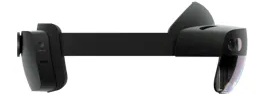
\includegraphics[width=10cm]{images/hololens.png}
    \caption{HoloLens 2 by Microsoft \citep{hololens_image}.}
    \label{fig:hololens}
\end{figure}

The HoloLens 2 is a mixed reality headset developed by Microsoft, it is designed to blend virtual objects with the real world in a seamless manner. It represents a significant advancement in augmented reality and, although released in 2019, is still considered to be at the forefront of mixed reality technology. The headset operates by utilizing a combination of sensors, cameras and holographic processing units which work in tandem to understand the physical environment and overlay digital content onto it in real time. The HoloLens has a wide range of capabilities including spatial mapping, gesture recognition and hand tracking, eye tracking and remote collaboration \citep{hololens}.

Building a Unity project to the HoloLens 2 requires specific settings in the Unity editor to be enabled and certain packages to be downloaded. The main downloads required are the Windows Development Kit and the Windows Mixed Reality Feature Pack. Both downloads contain vital software for the building and deploying of Unity applications on the HoloLens 2. Once the Unity application is built to the HoloLens it can be ran using the menu inside the HoloLens.

The HoloLens was chosen for this project as it offers a slim and sleek design which allows for as little interference with the cyclist as possible, ensuring that safety is upheld during the use of the prototype. The only downside to using the HoloLens 2 is the cost. Microsoft has not made the HoloLens commercially available and instead, due to the high cost, it is marketed towards large companies and researchers looking to develop software for the headset. When considering the future of large scale usage of a prototype such as this, the cost will have to drastically fall before it becomes commercially available and affordable for cyclists around the world.

%==================================================================================================================================
\chapter{Evaluation}

\section{Testing}

To ensure that the prototype was in a working and finished state, testing was required to be carried out. Unfortunately, for safety reasons, I was unable to test the prototype whilst out on a public road. Instead I opted to test the project from a stationary point of view, looking at a car from multiple different views and mimicking a cyclists positioning on the road. All four designs were tested, the two side designs and two rear designs, and screenshots were taken through the HoloLens headset of the view that the cyclist would see whilst interacting with an autonomous vehicle. Figures \ref{fig:real_side_1}, \ref{fig:real_side_2} and \ref{fig:real_side_3} show the images of the first side design in testing. Figures \ref{fig:real_side_4}, \ref{fig:real_side_5} and \ref{fig:real_side_6} show the second side design in testing. Figures \ref{fig:real_rear_1}, \ref{fig:real_rear_2} and \ref{fig:real_rear_3} show the images of first rear design in testing. Finally, Figures \ref{fig:real_rear_4}, \ref{fig:real_rear_5} and \ref{fig:real_rear_6} show the second rear design in testing.

\begin{figure}[H]
    \centering
    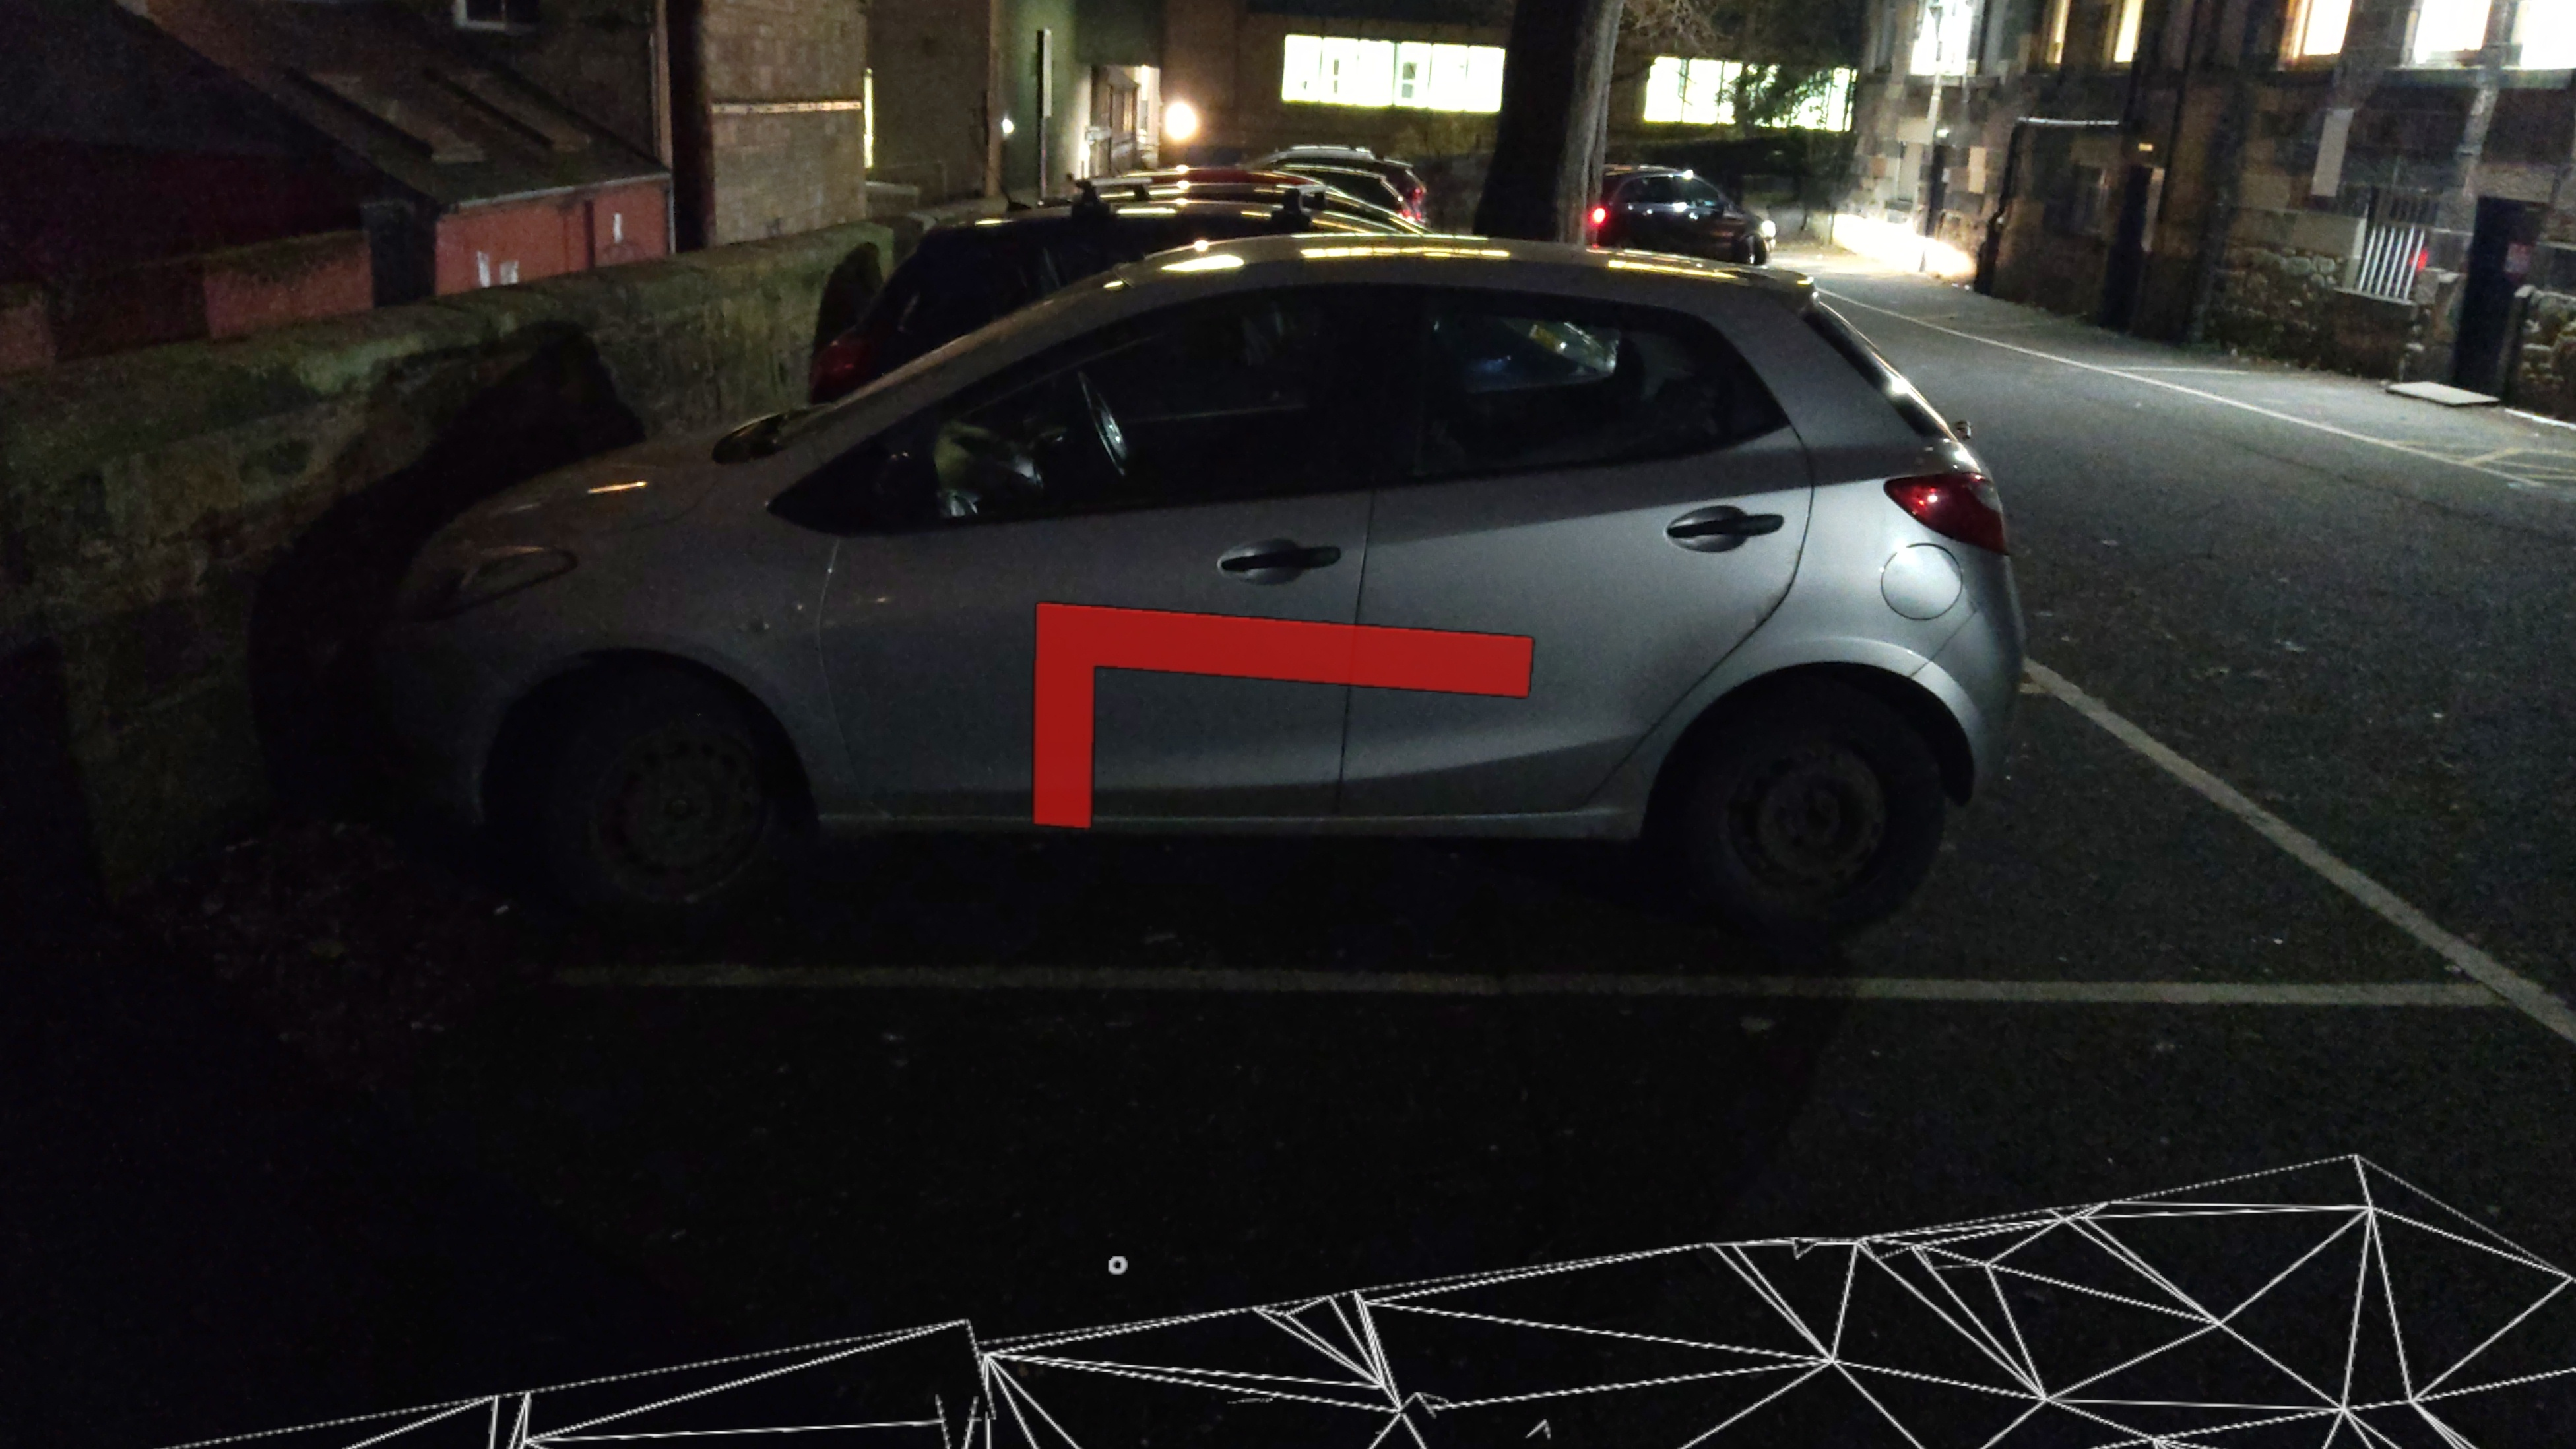
\includegraphics[width=10cm]{images/001.jpg}
    \caption{Side Design 1 Red.}
    \label{fig:real_side_1}
\end{figure}

\begin{figure}[H]
    \centering
    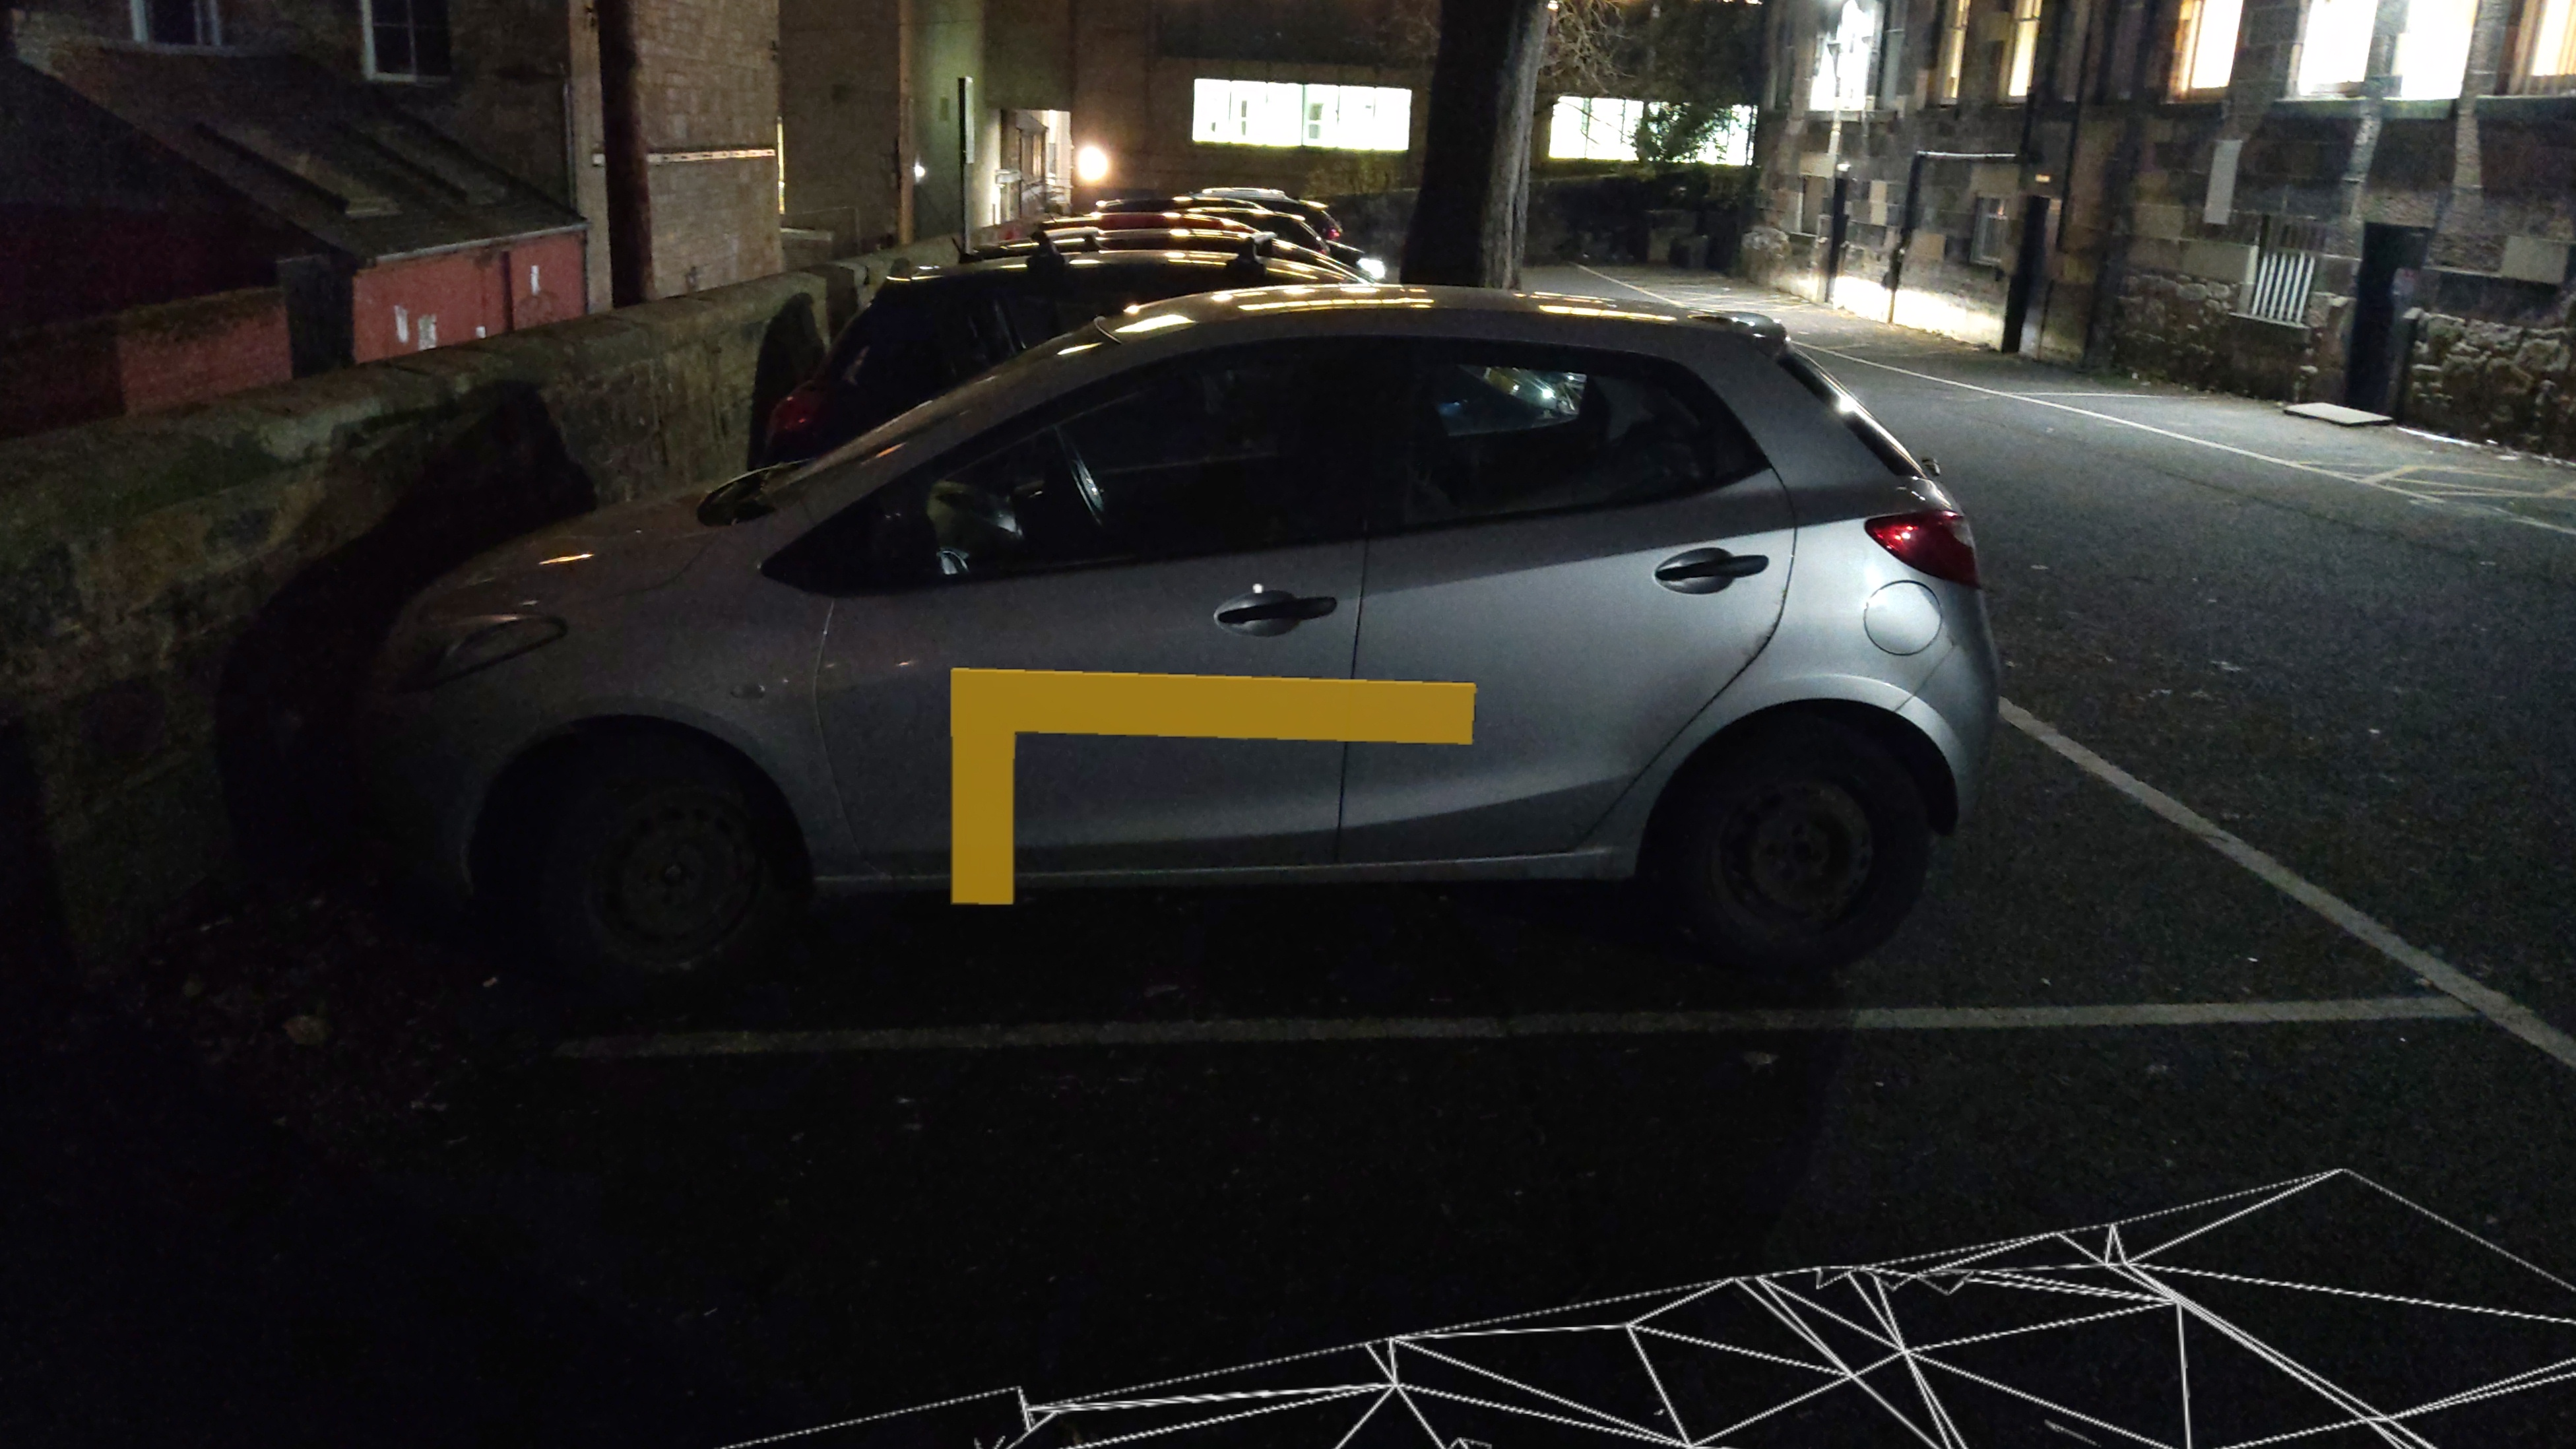
\includegraphics[width=10cm]{images/002.jpg}
    \caption{Side Design 1 Amber.}
    \label{fig:real_side_2}
\end{figure}

\begin{figure}[H]
    \centering
    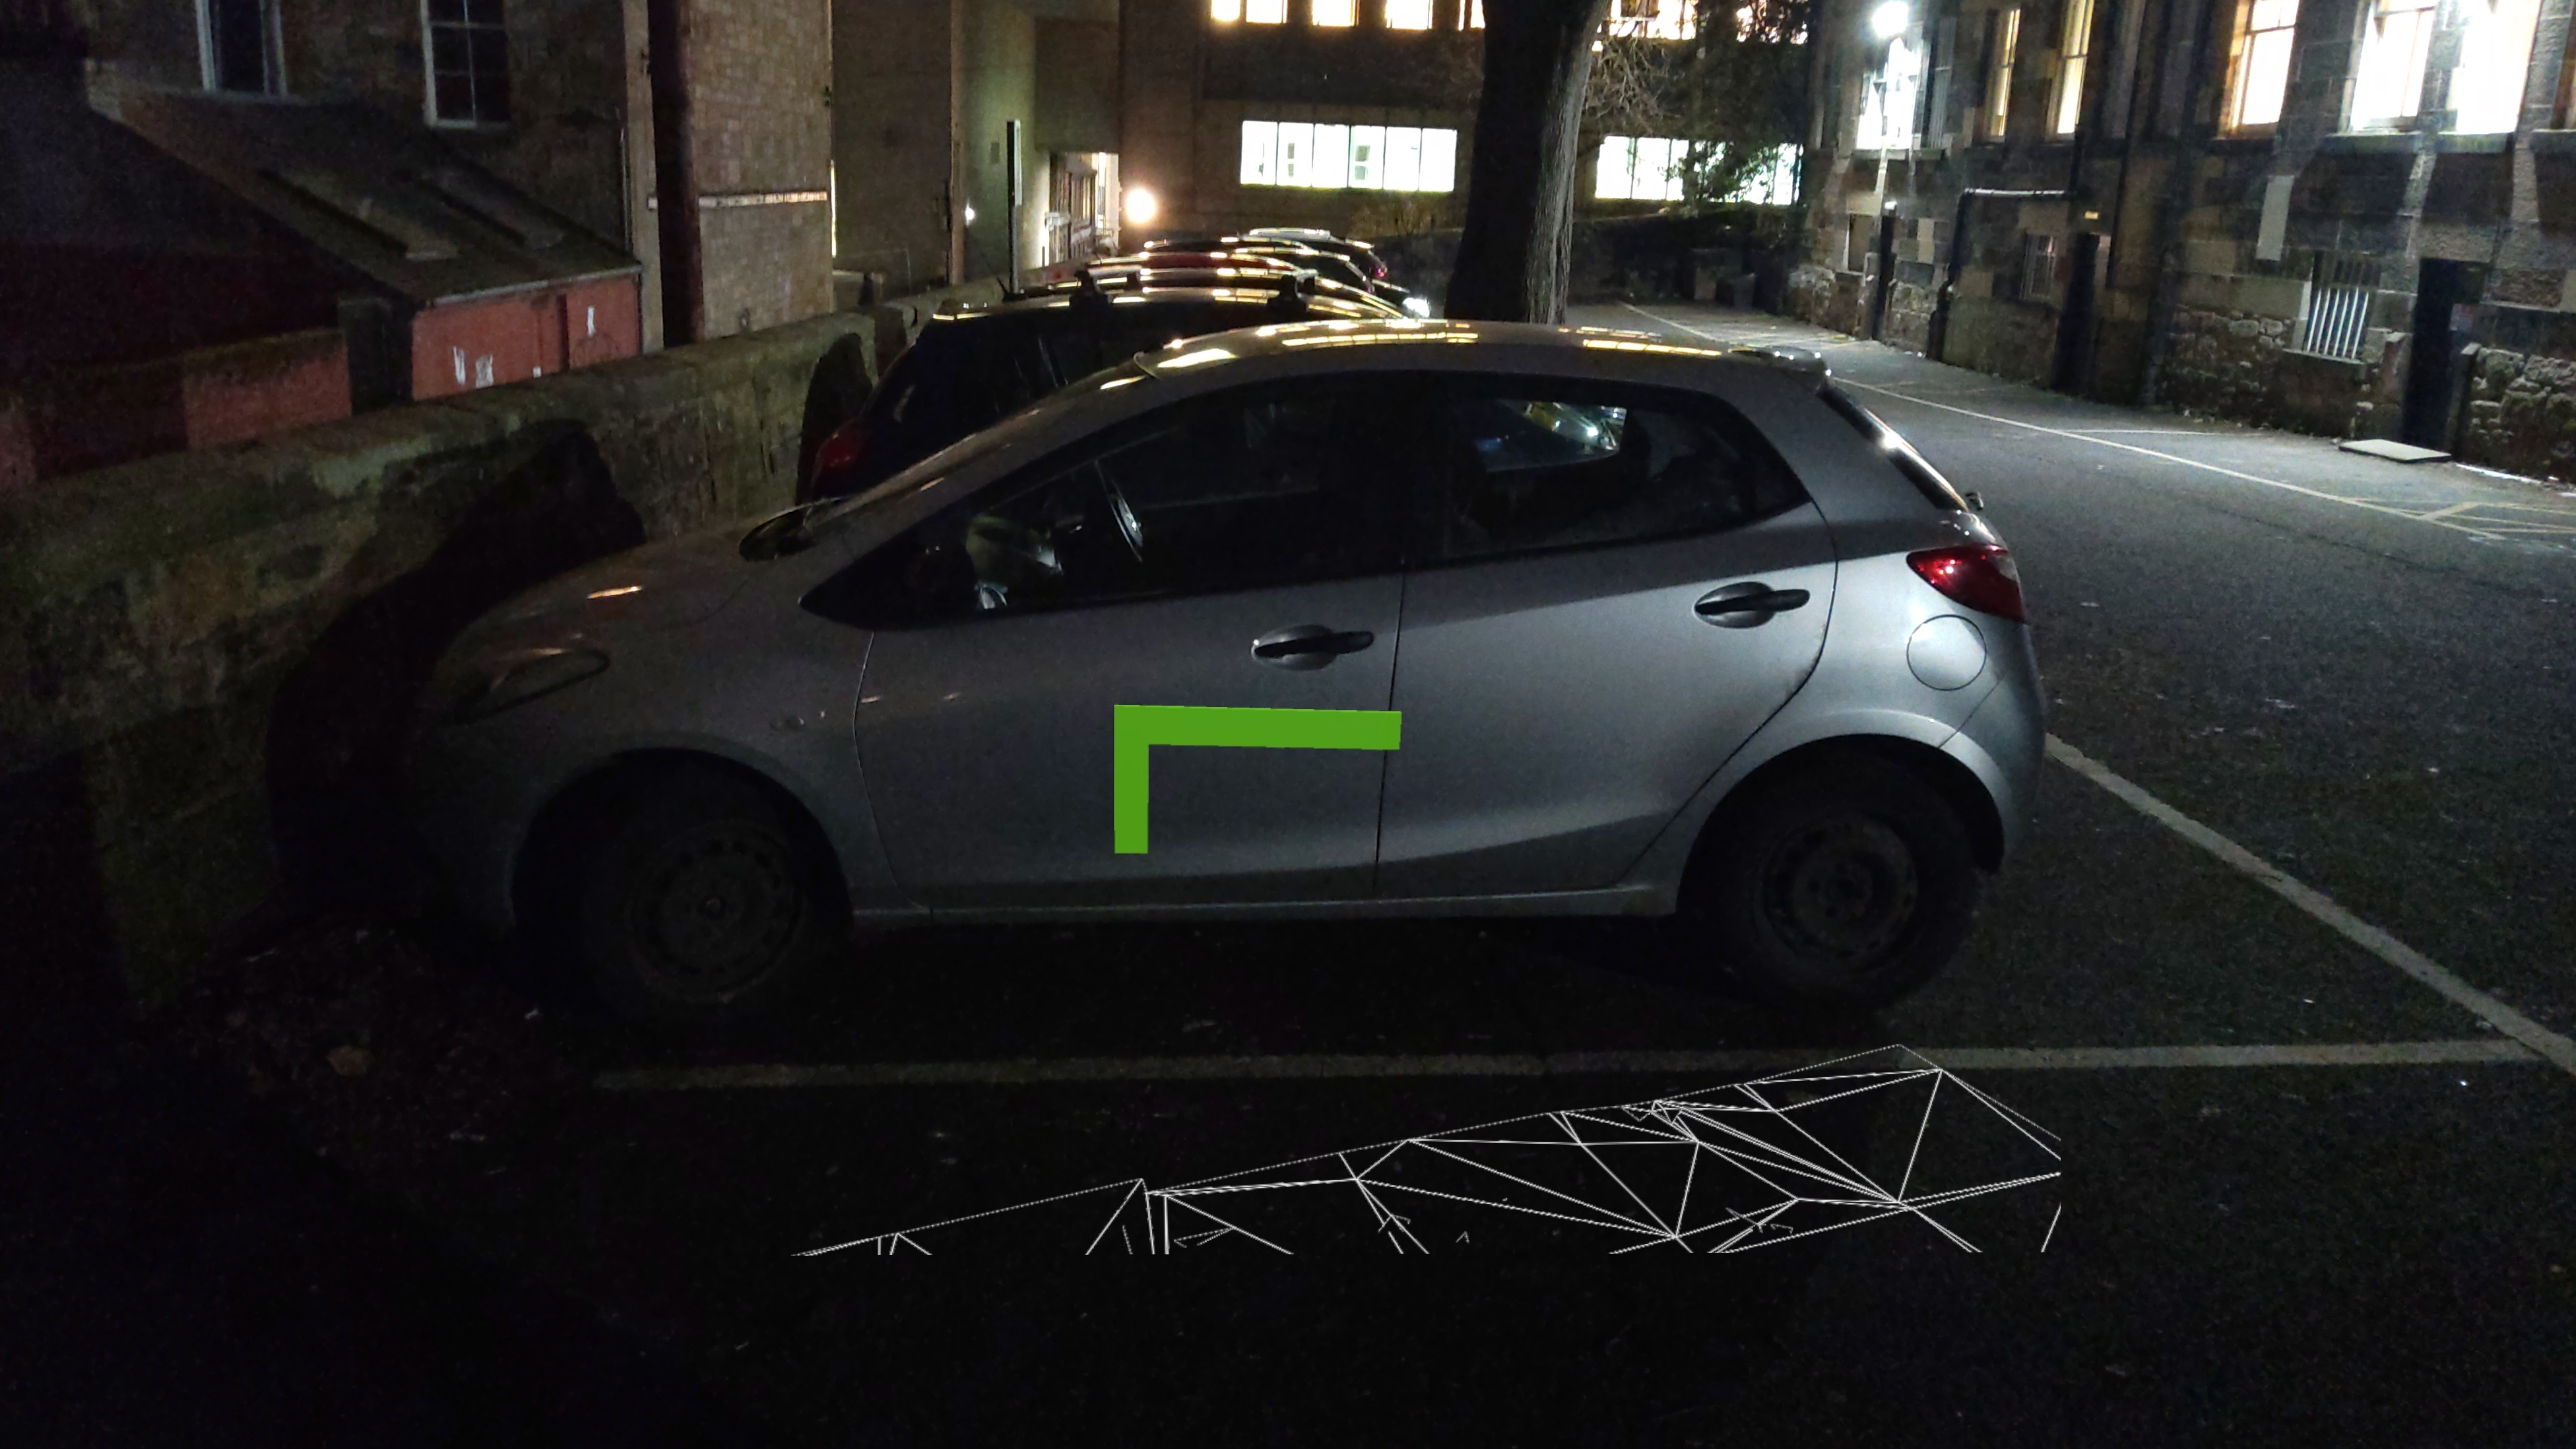
\includegraphics[width=10cm]{images/003.jpg}
    \caption{Side Design 1 Green.}
    \label{fig:real_side_3}
\end{figure}

\begin{figure}[H]
    \centering
    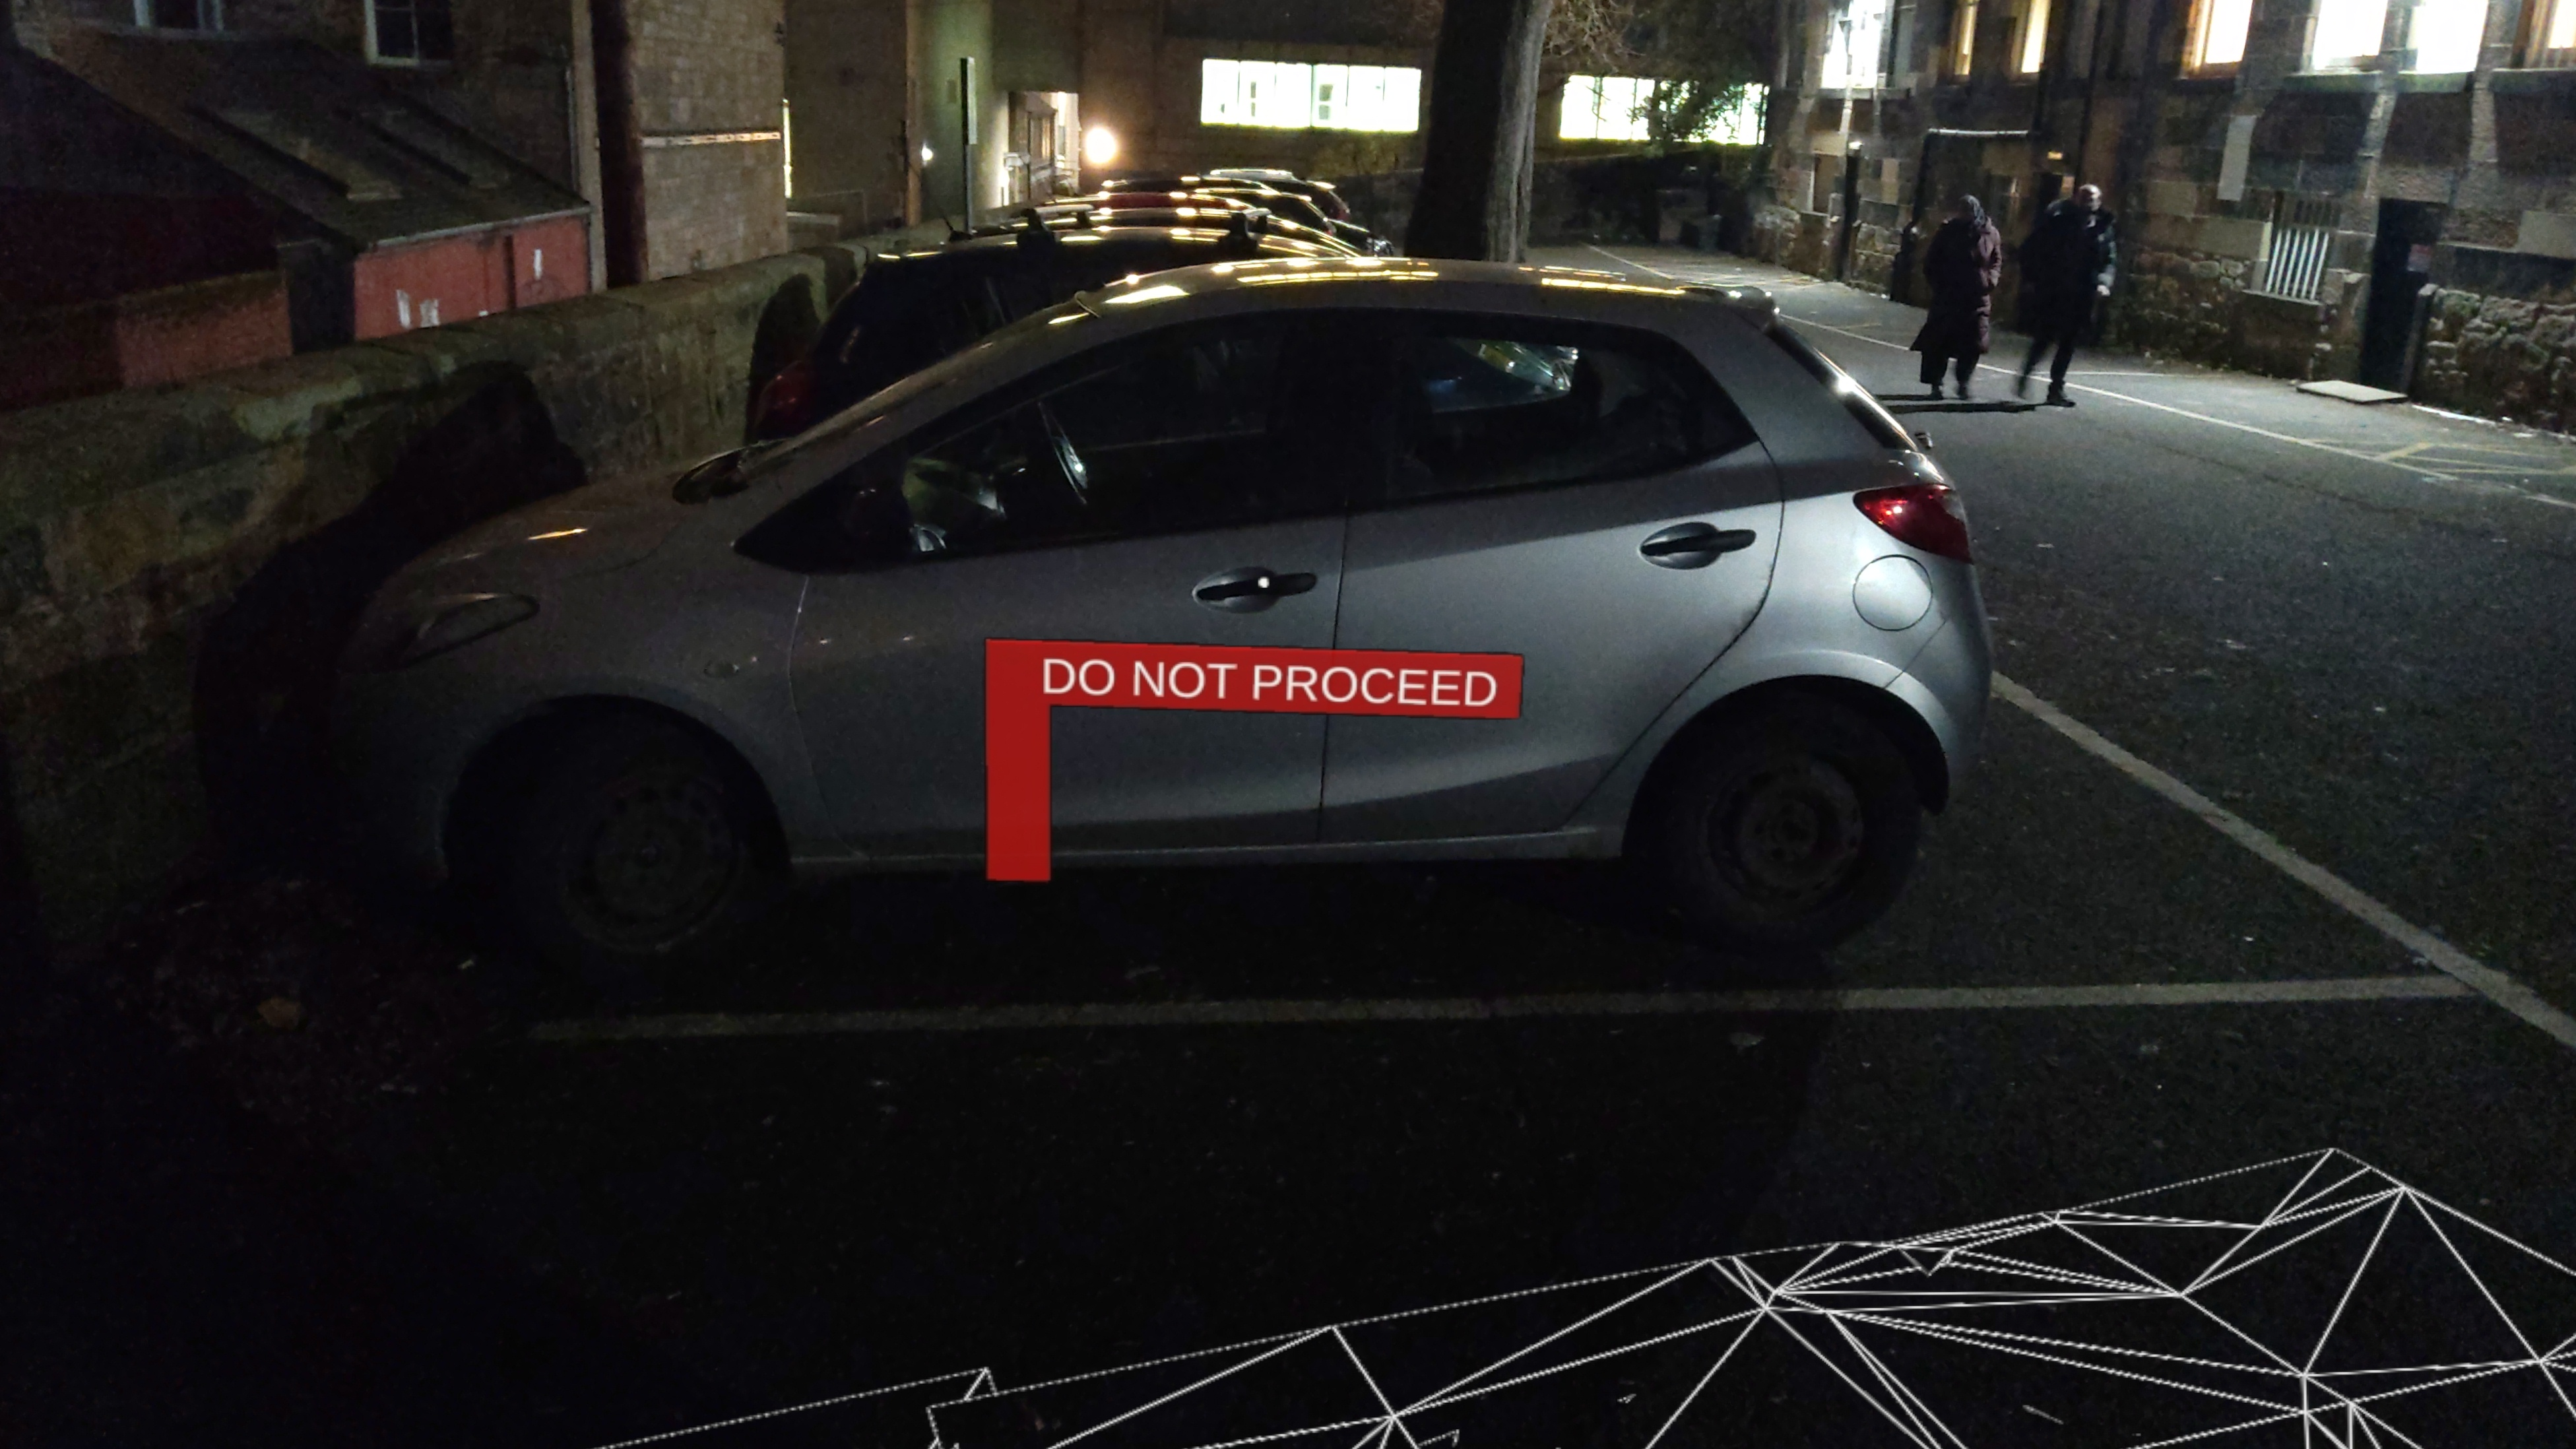
\includegraphics[width=10cm]{images/004.jpg}
    \caption{Side Design 2 Red.}
    \label{fig:real_side_4}
\end{figure}

\begin{figure}[H]
    \centering
    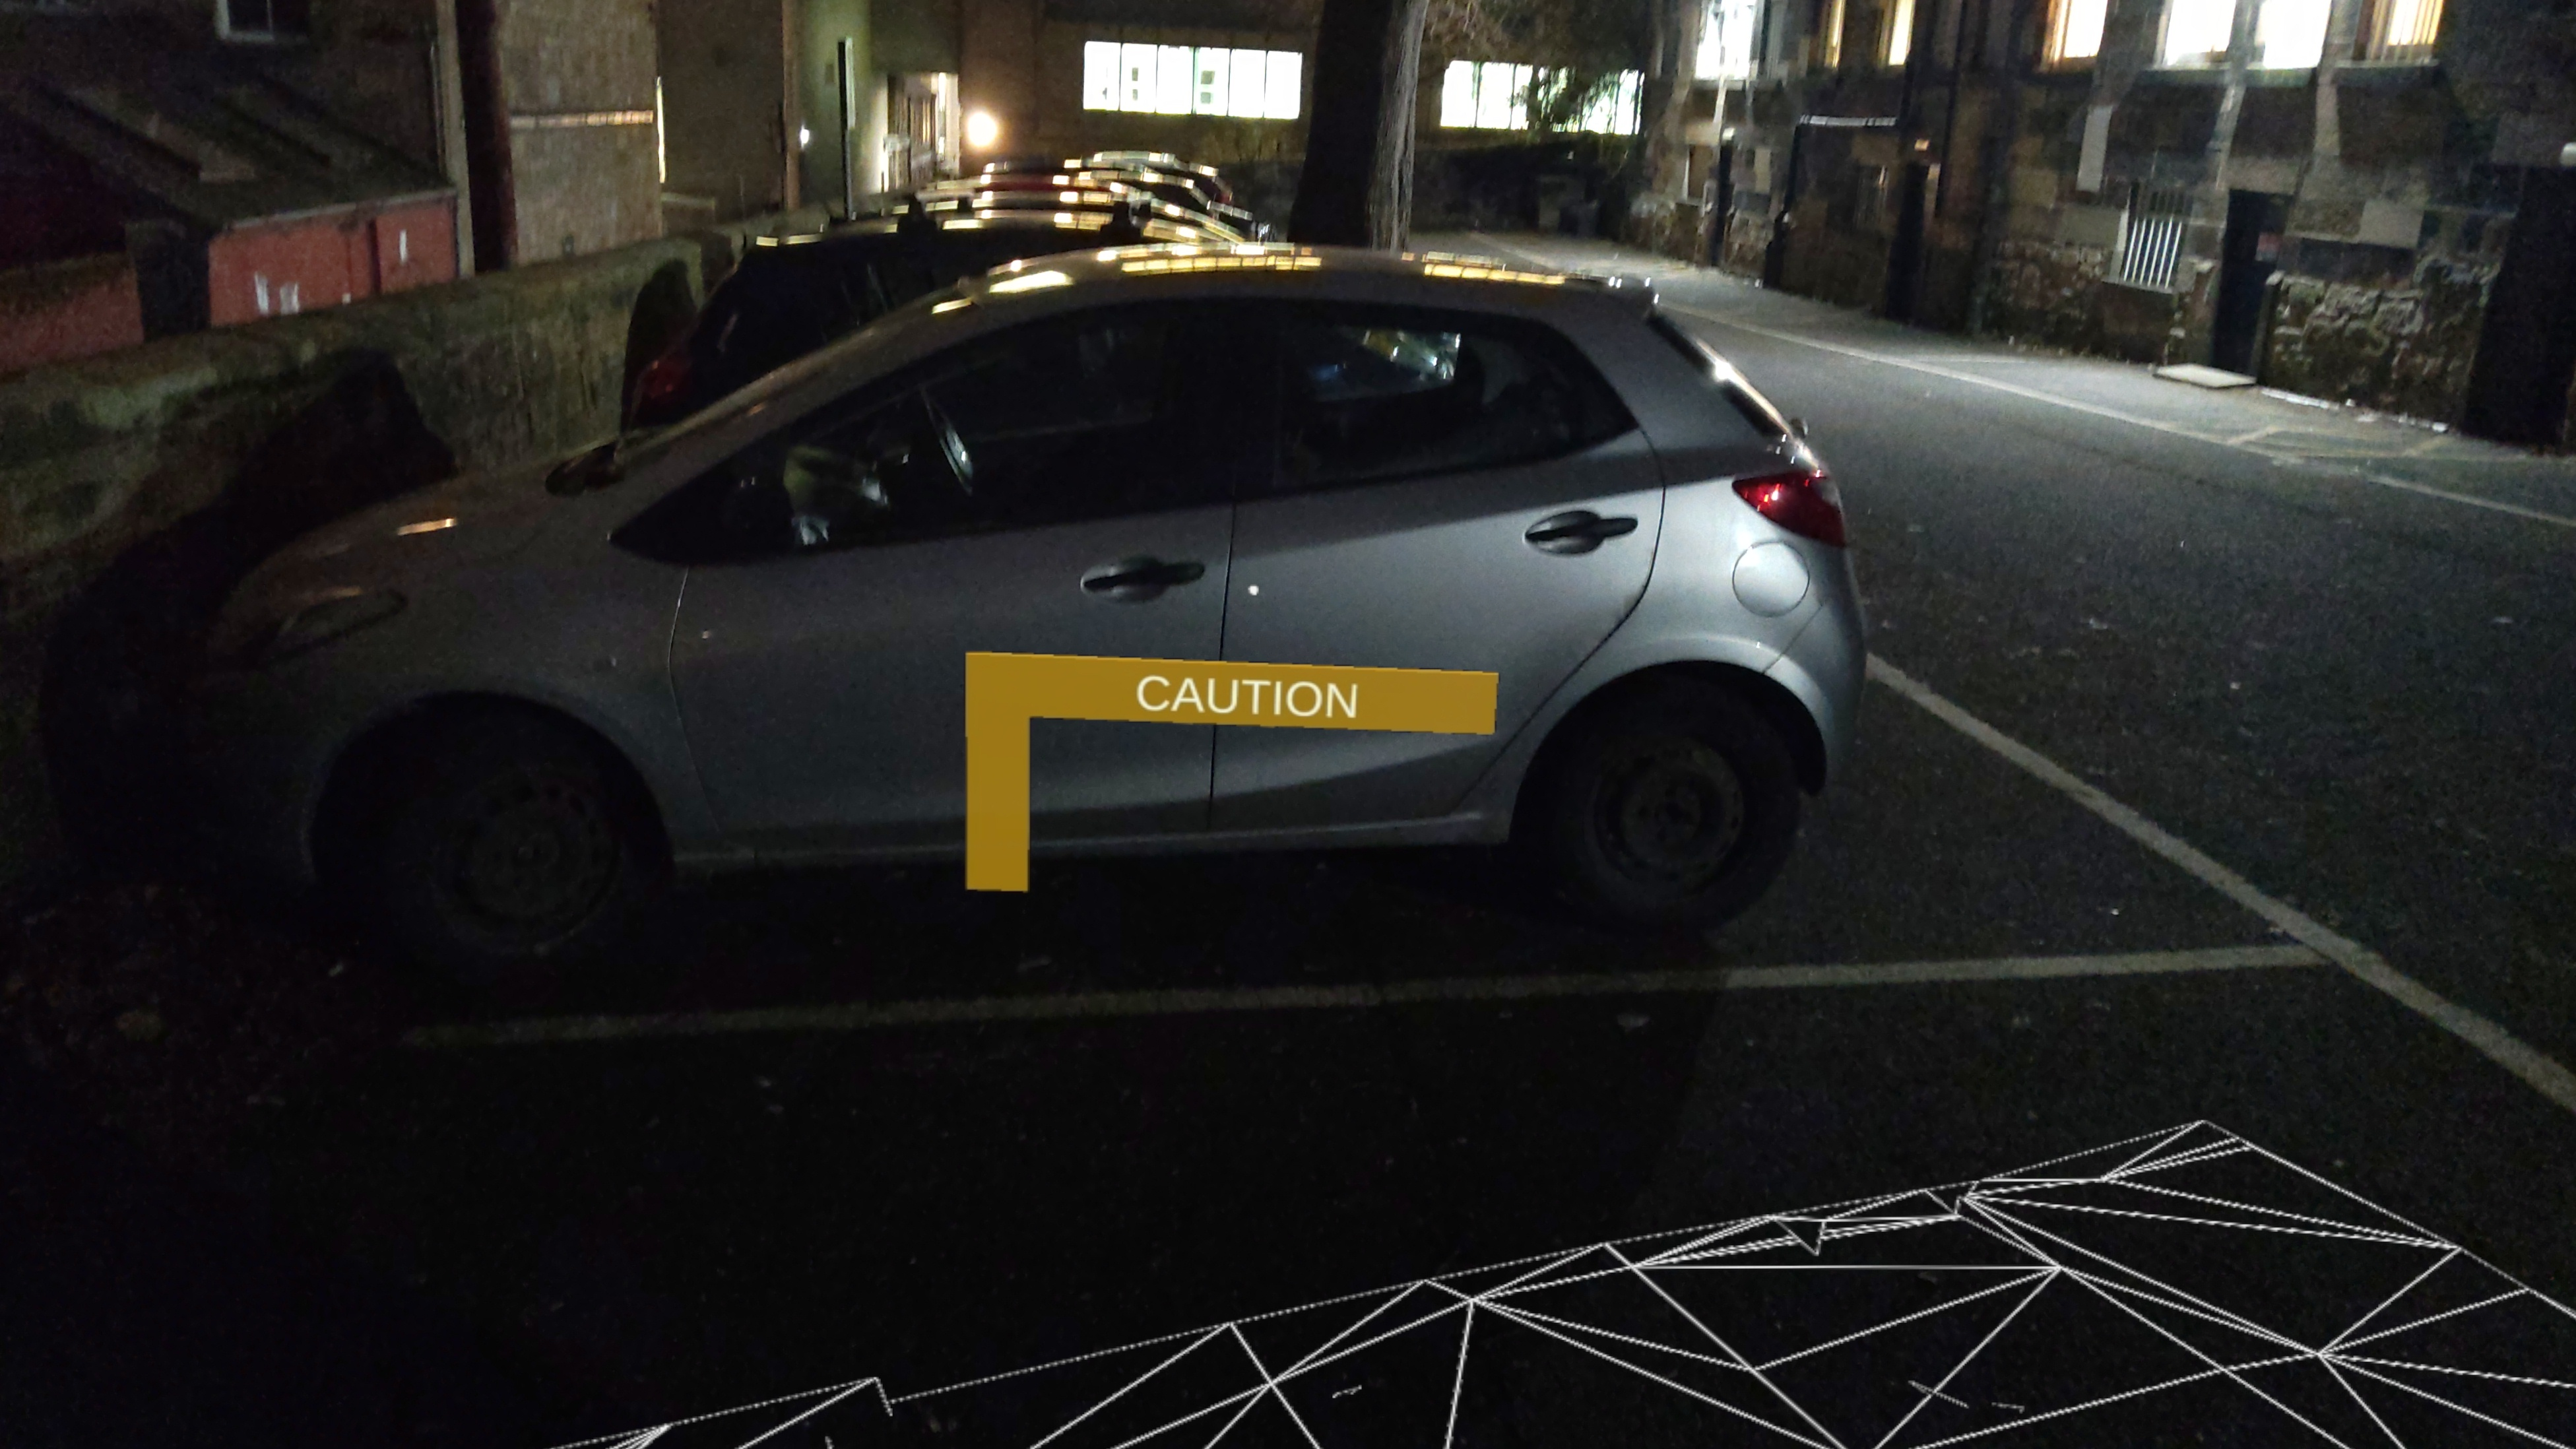
\includegraphics[width=10cm]{images/005.jpg}
    \caption{Side Design 2 Amber.}
    \label{fig:real_side_5}
\end{figure}

\begin{figure}[H]
    \centering
    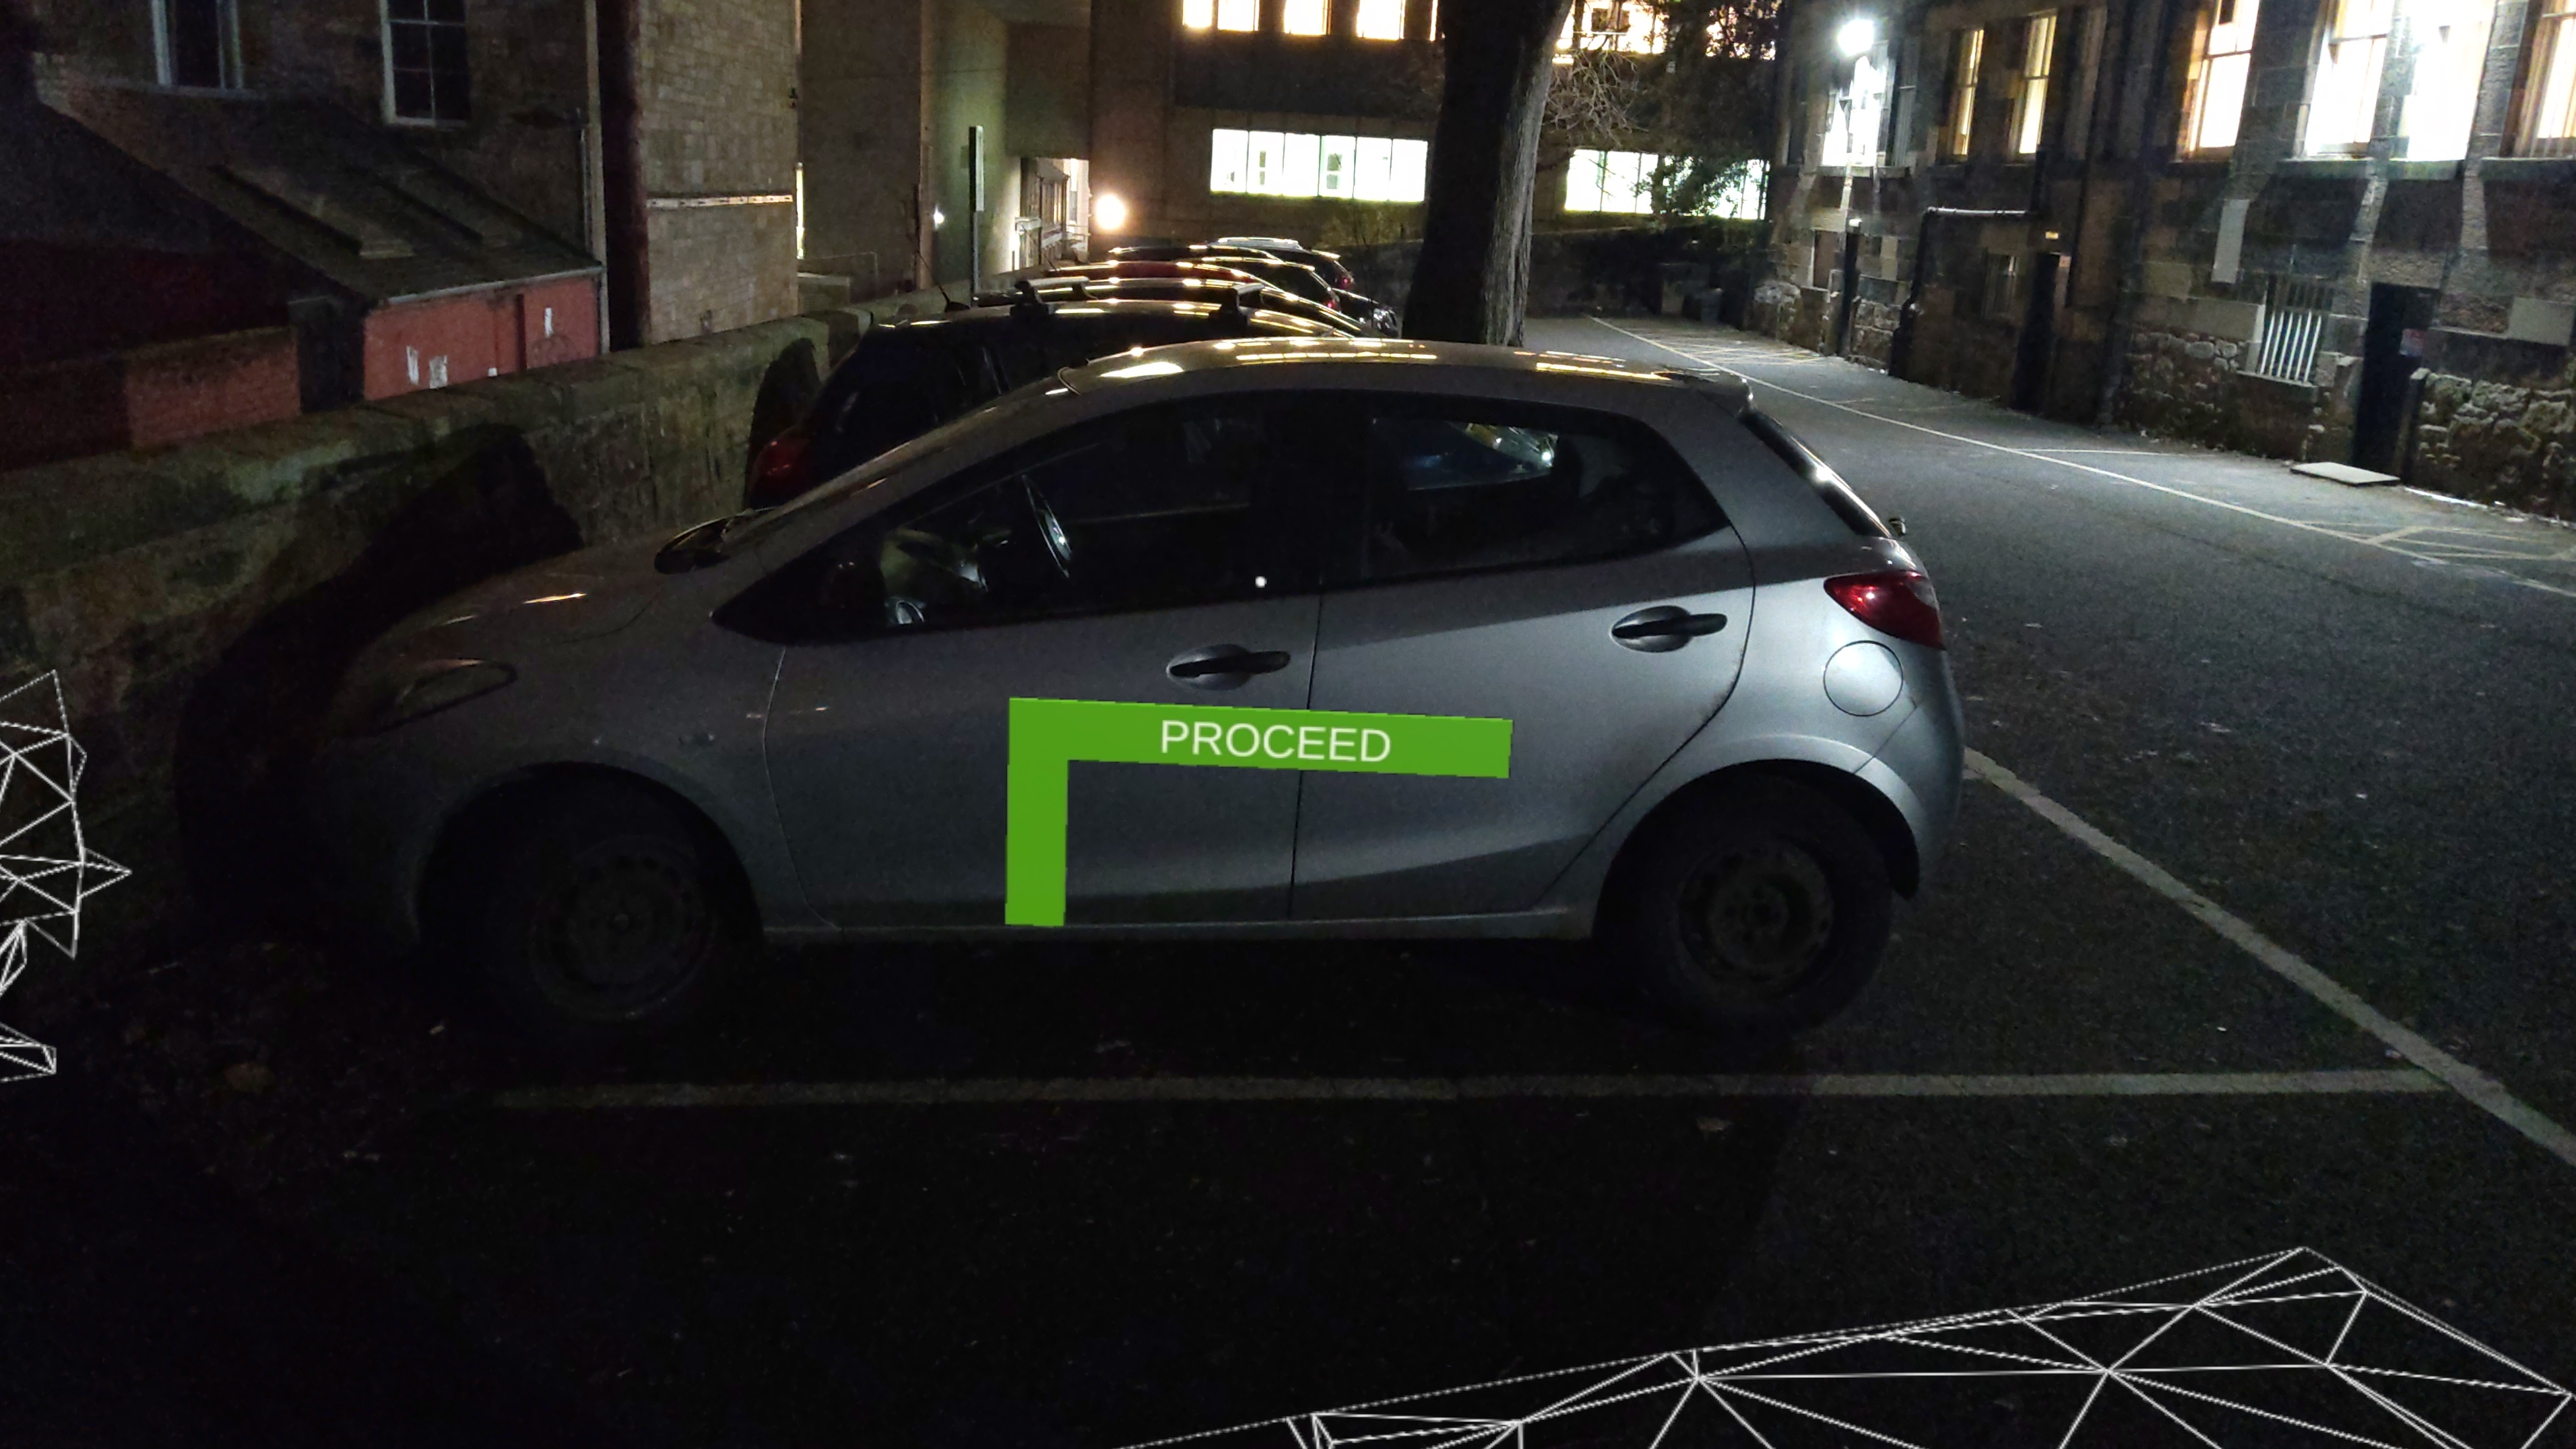
\includegraphics[width=10cm]{images/006.jpg}
    \caption{Side Design 2 Green.}
    \label{fig:real_side_6}
\end{figure}

\begin{figure}[H]
    \centering
    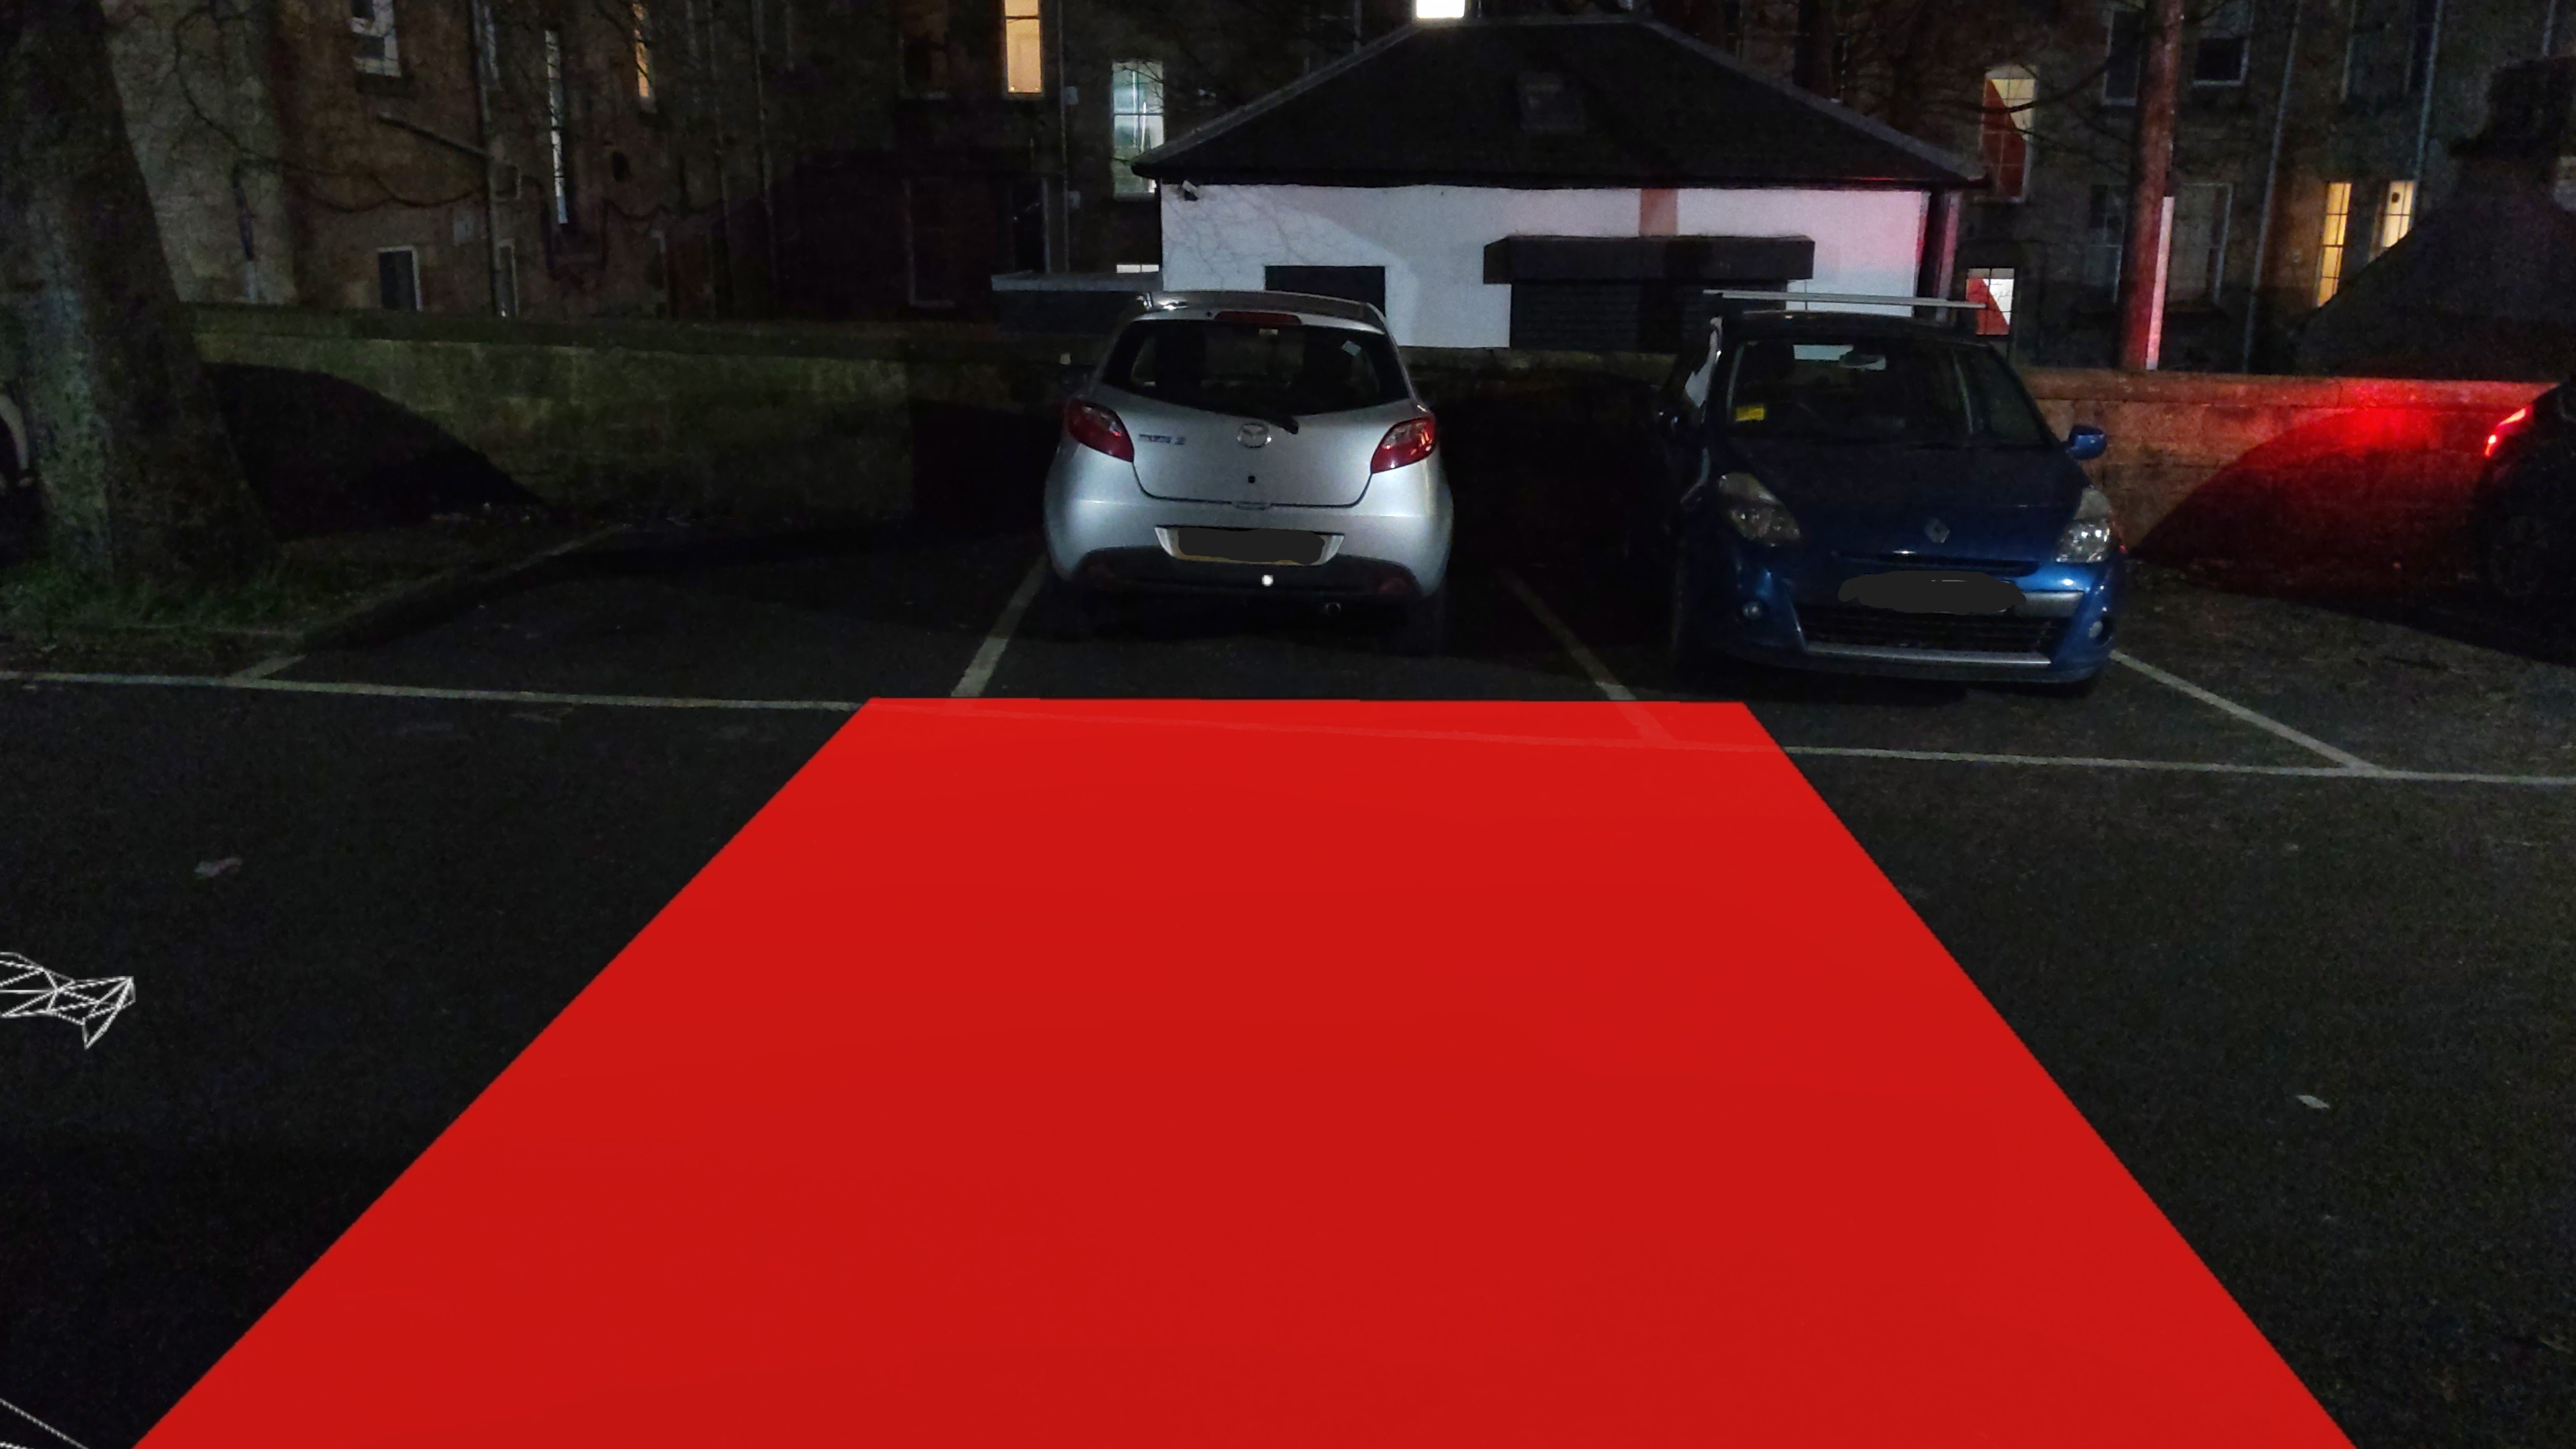
\includegraphics[width=10cm]{images/design1.1.jpg}
    \caption{Rear Design 1 Red.}
    \label{fig:real_rear_1}
\end{figure}

\begin{figure}[H]
    \centering
    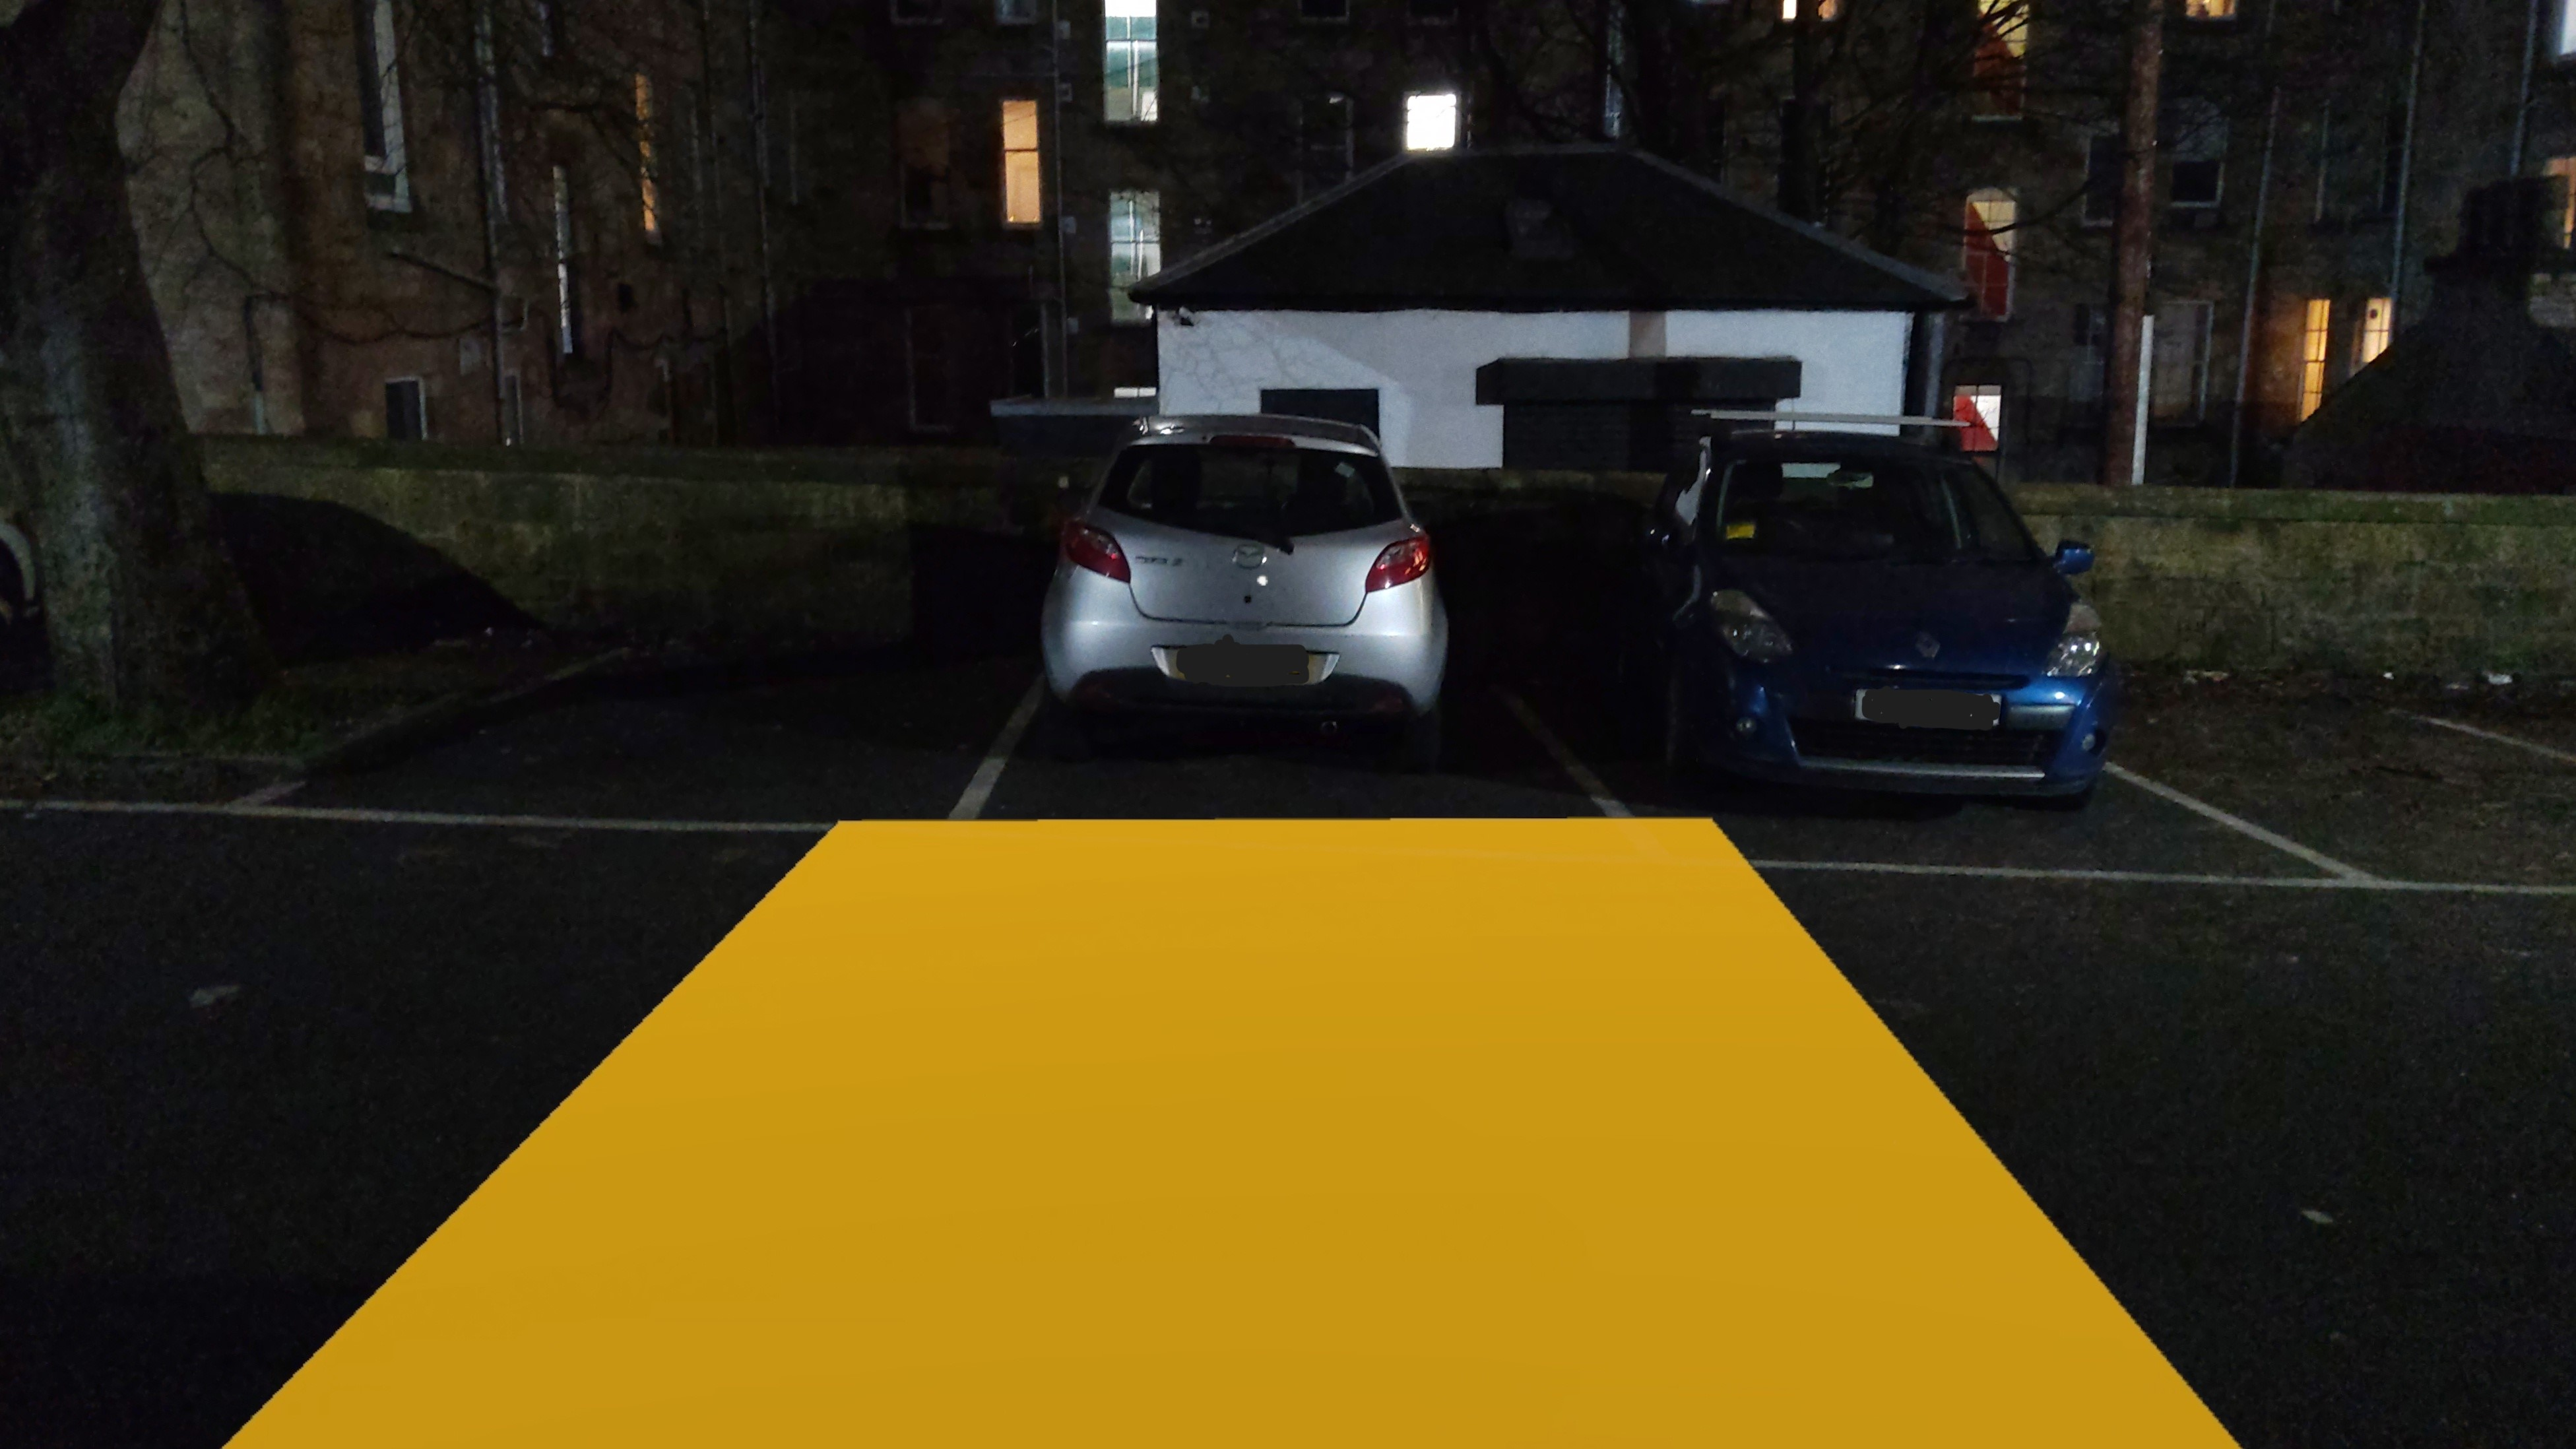
\includegraphics[width=10cm]{images/design1.2.jpg}
    \caption{Rear Design 1 Amber.}
    \label{fig:real_rear_2}
\end{figure}

\begin{figure}[H]
    \centering
    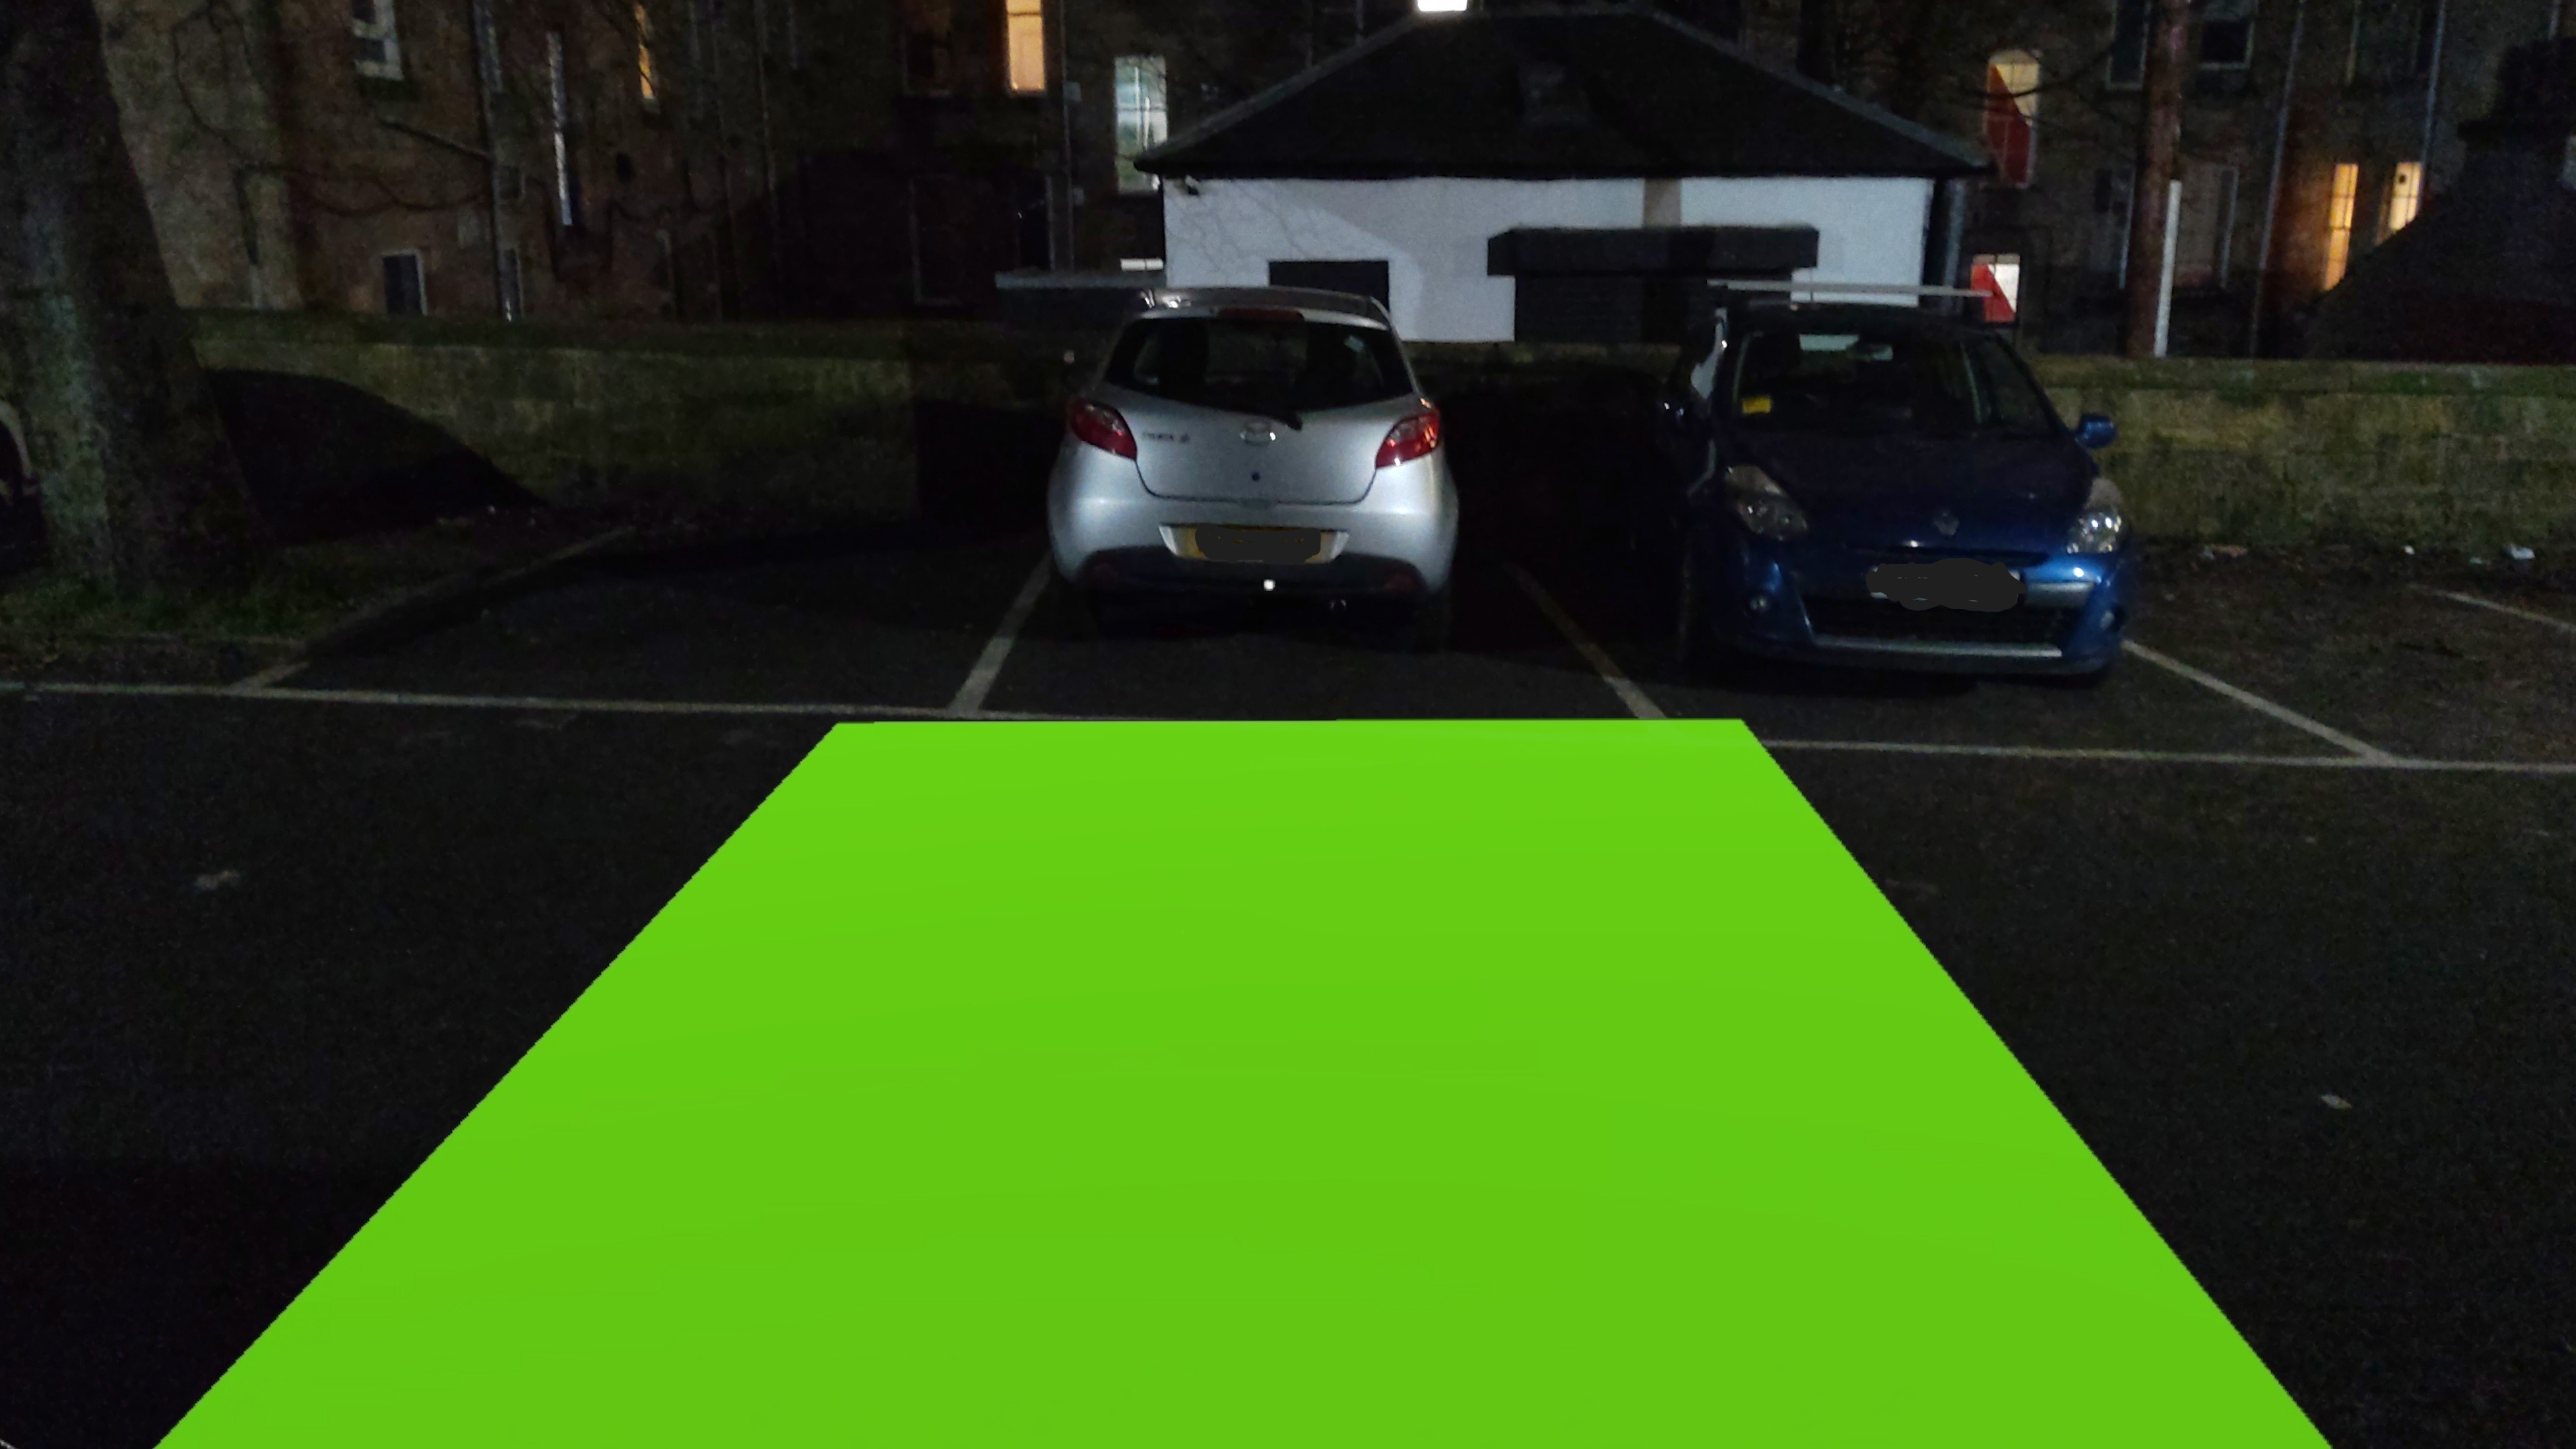
\includegraphics[width=10cm]{images/design1.3.jpg}
    \caption{Rear Design 1 Green.}
    \label{fig:real_rear_3}
\end{figure}

\begin{figure}[H]
    \centering
    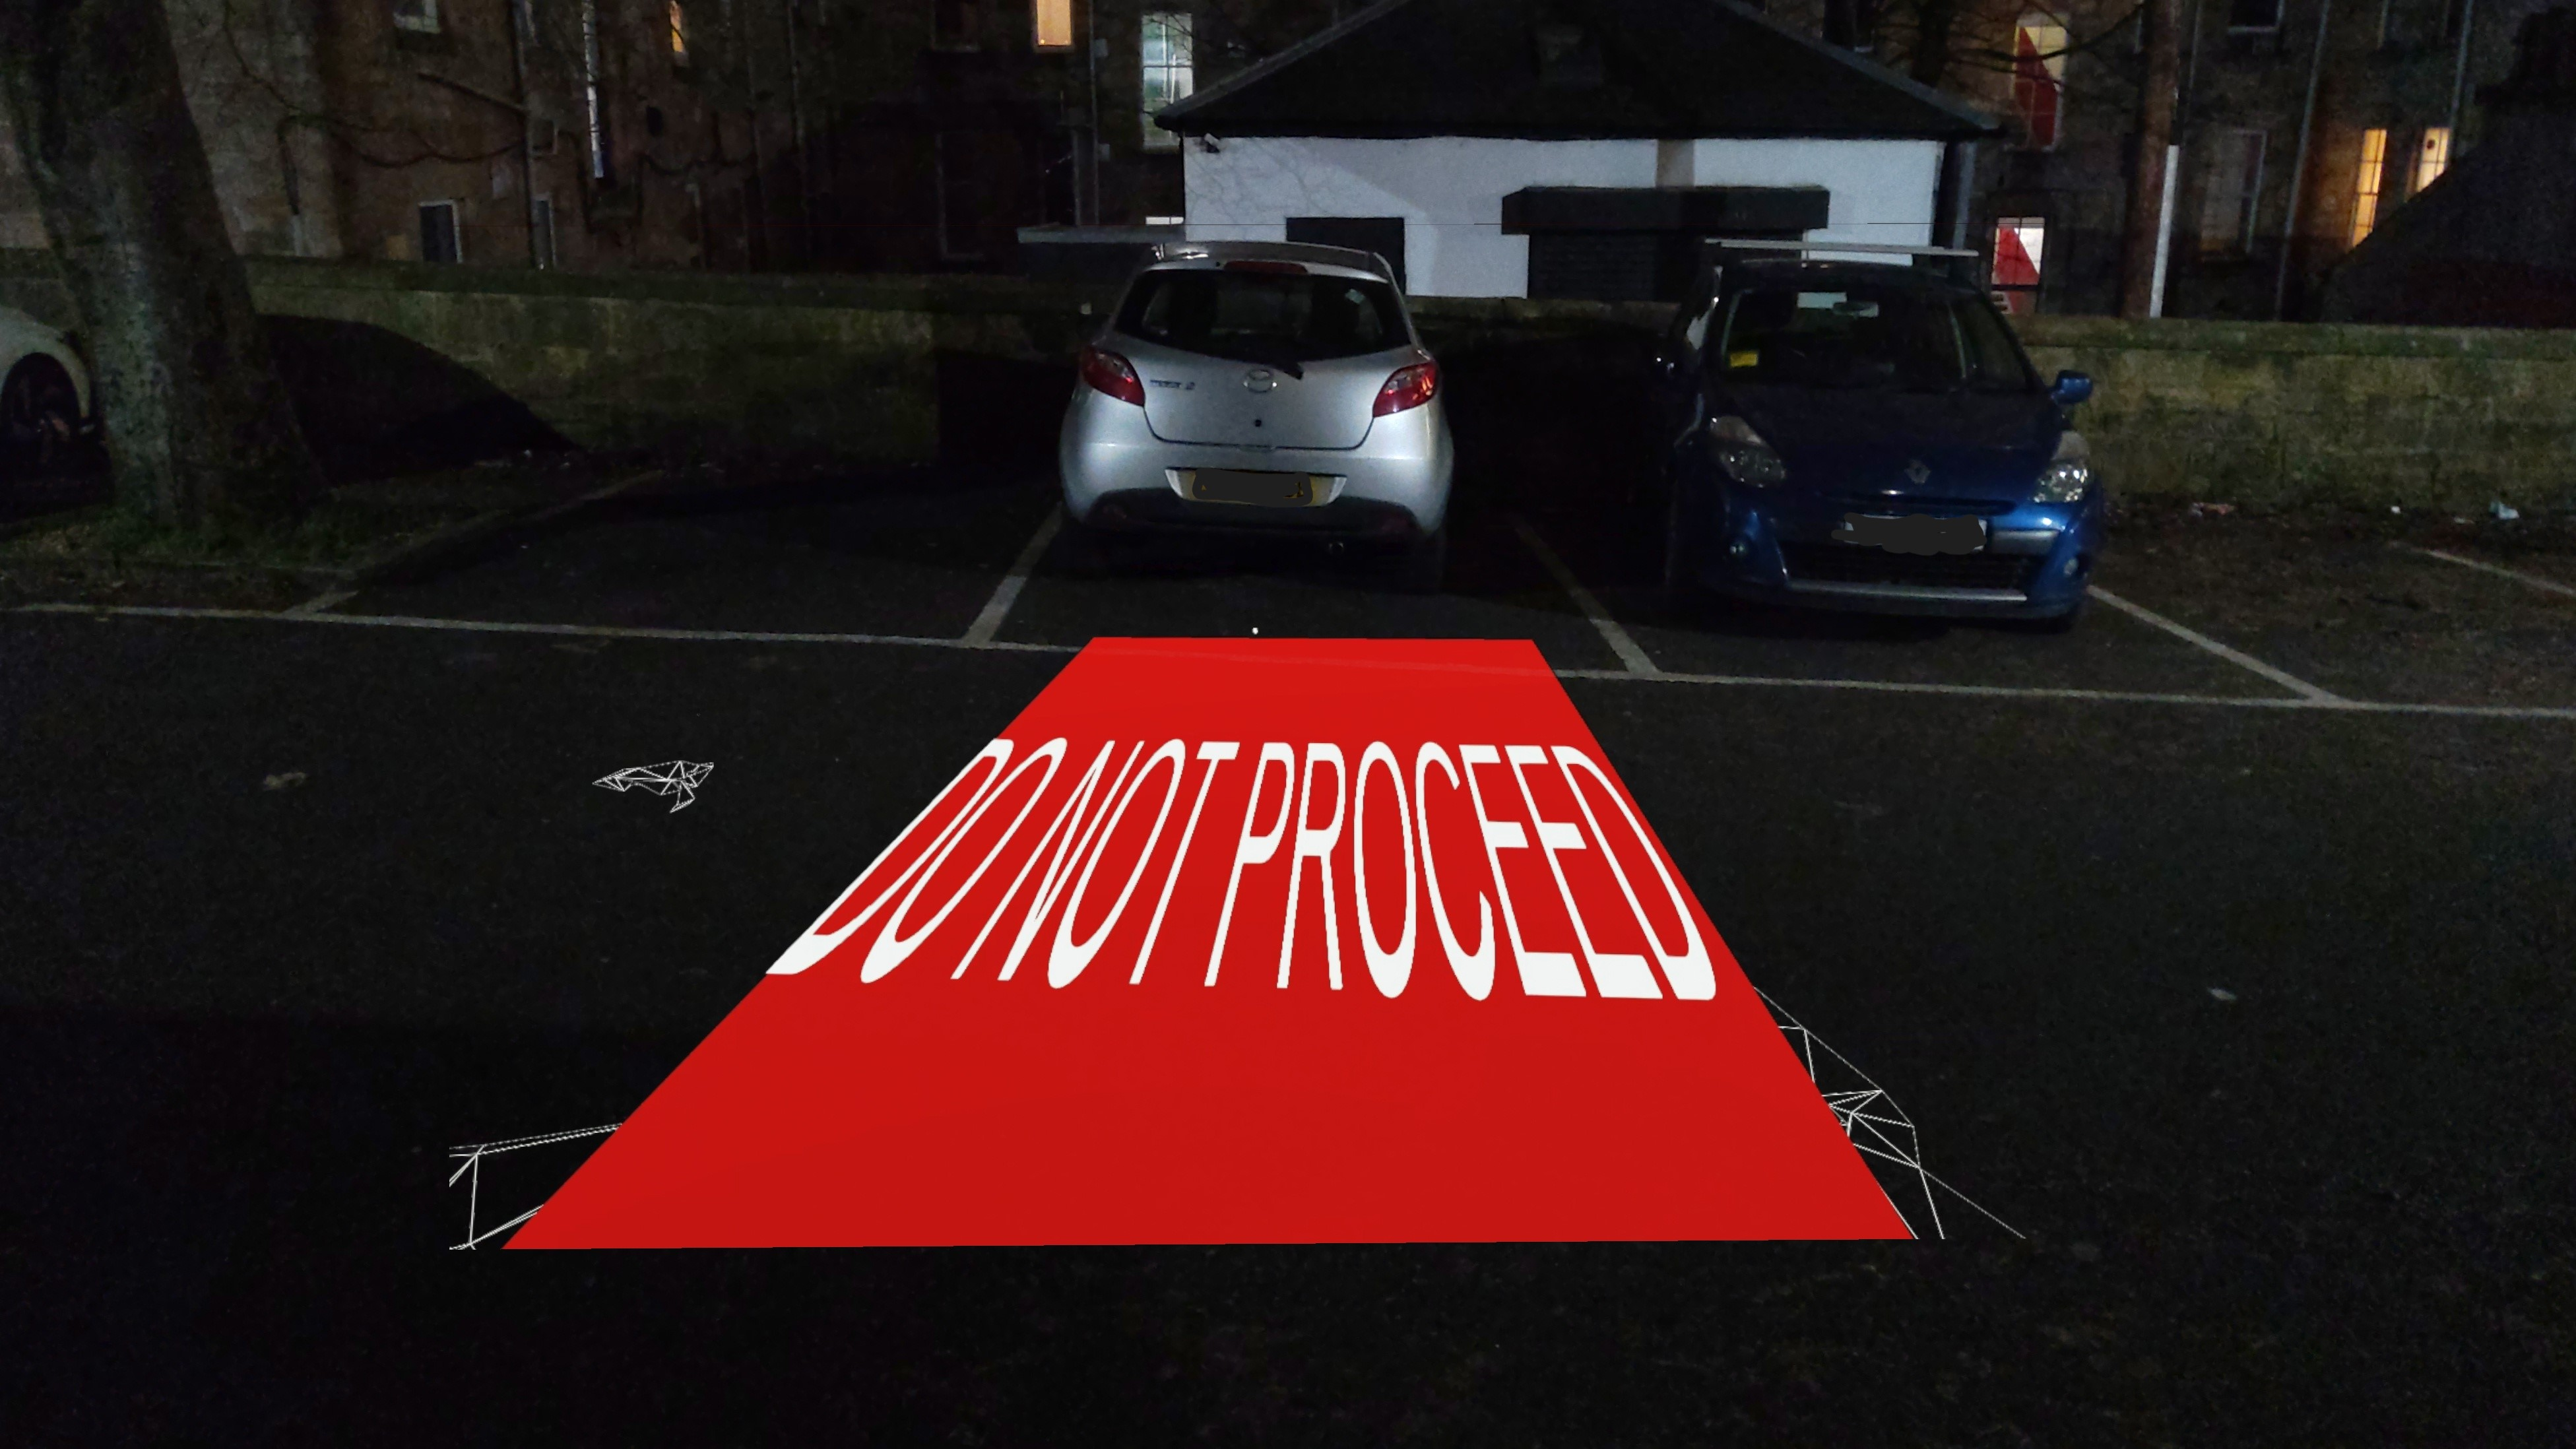
\includegraphics[width=10cm]{images/design2.1.jpg}
    \caption{Rear Design 2 Red.}
    \label{fig:real_rear_4}
\end{figure}

\begin{figure}[H]
    \centering
    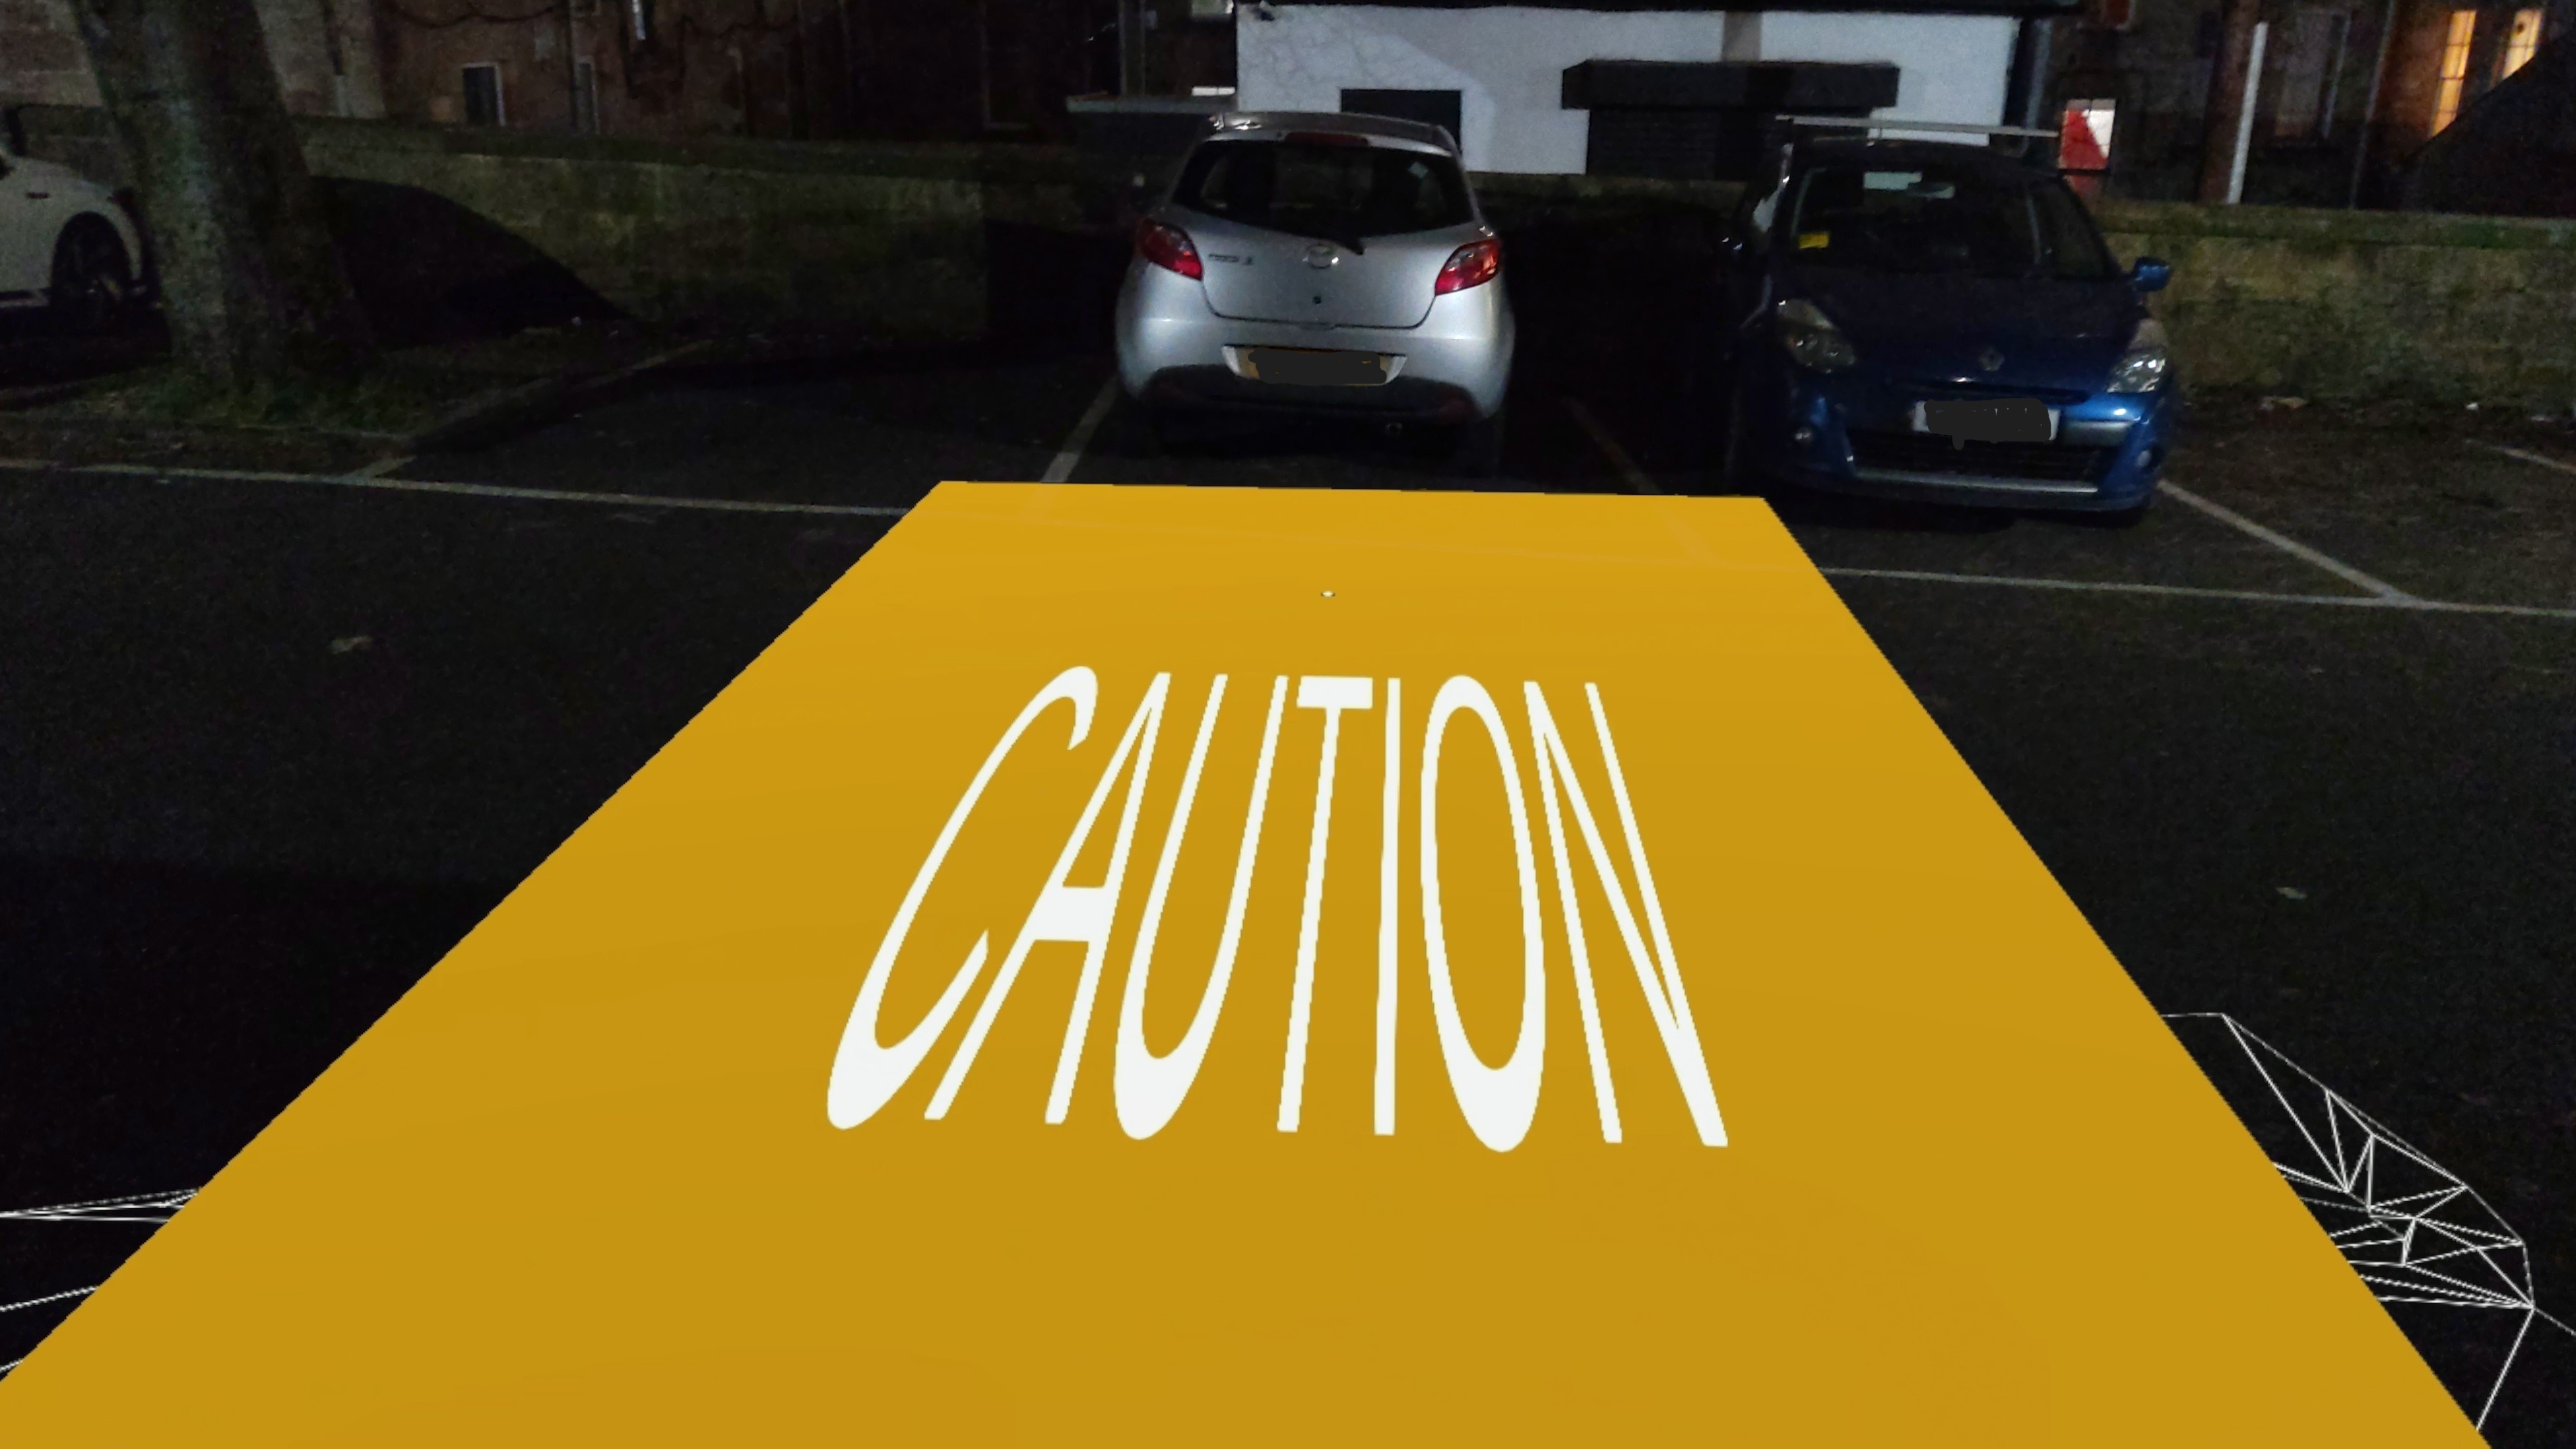
\includegraphics[width=10cm]{images/design2.2.jpg}
    \caption{Rear Design 2 Amber.}
    \label{fig:real_rear_5}
\end{figure}

\begin{figure}[H]
    \centering
    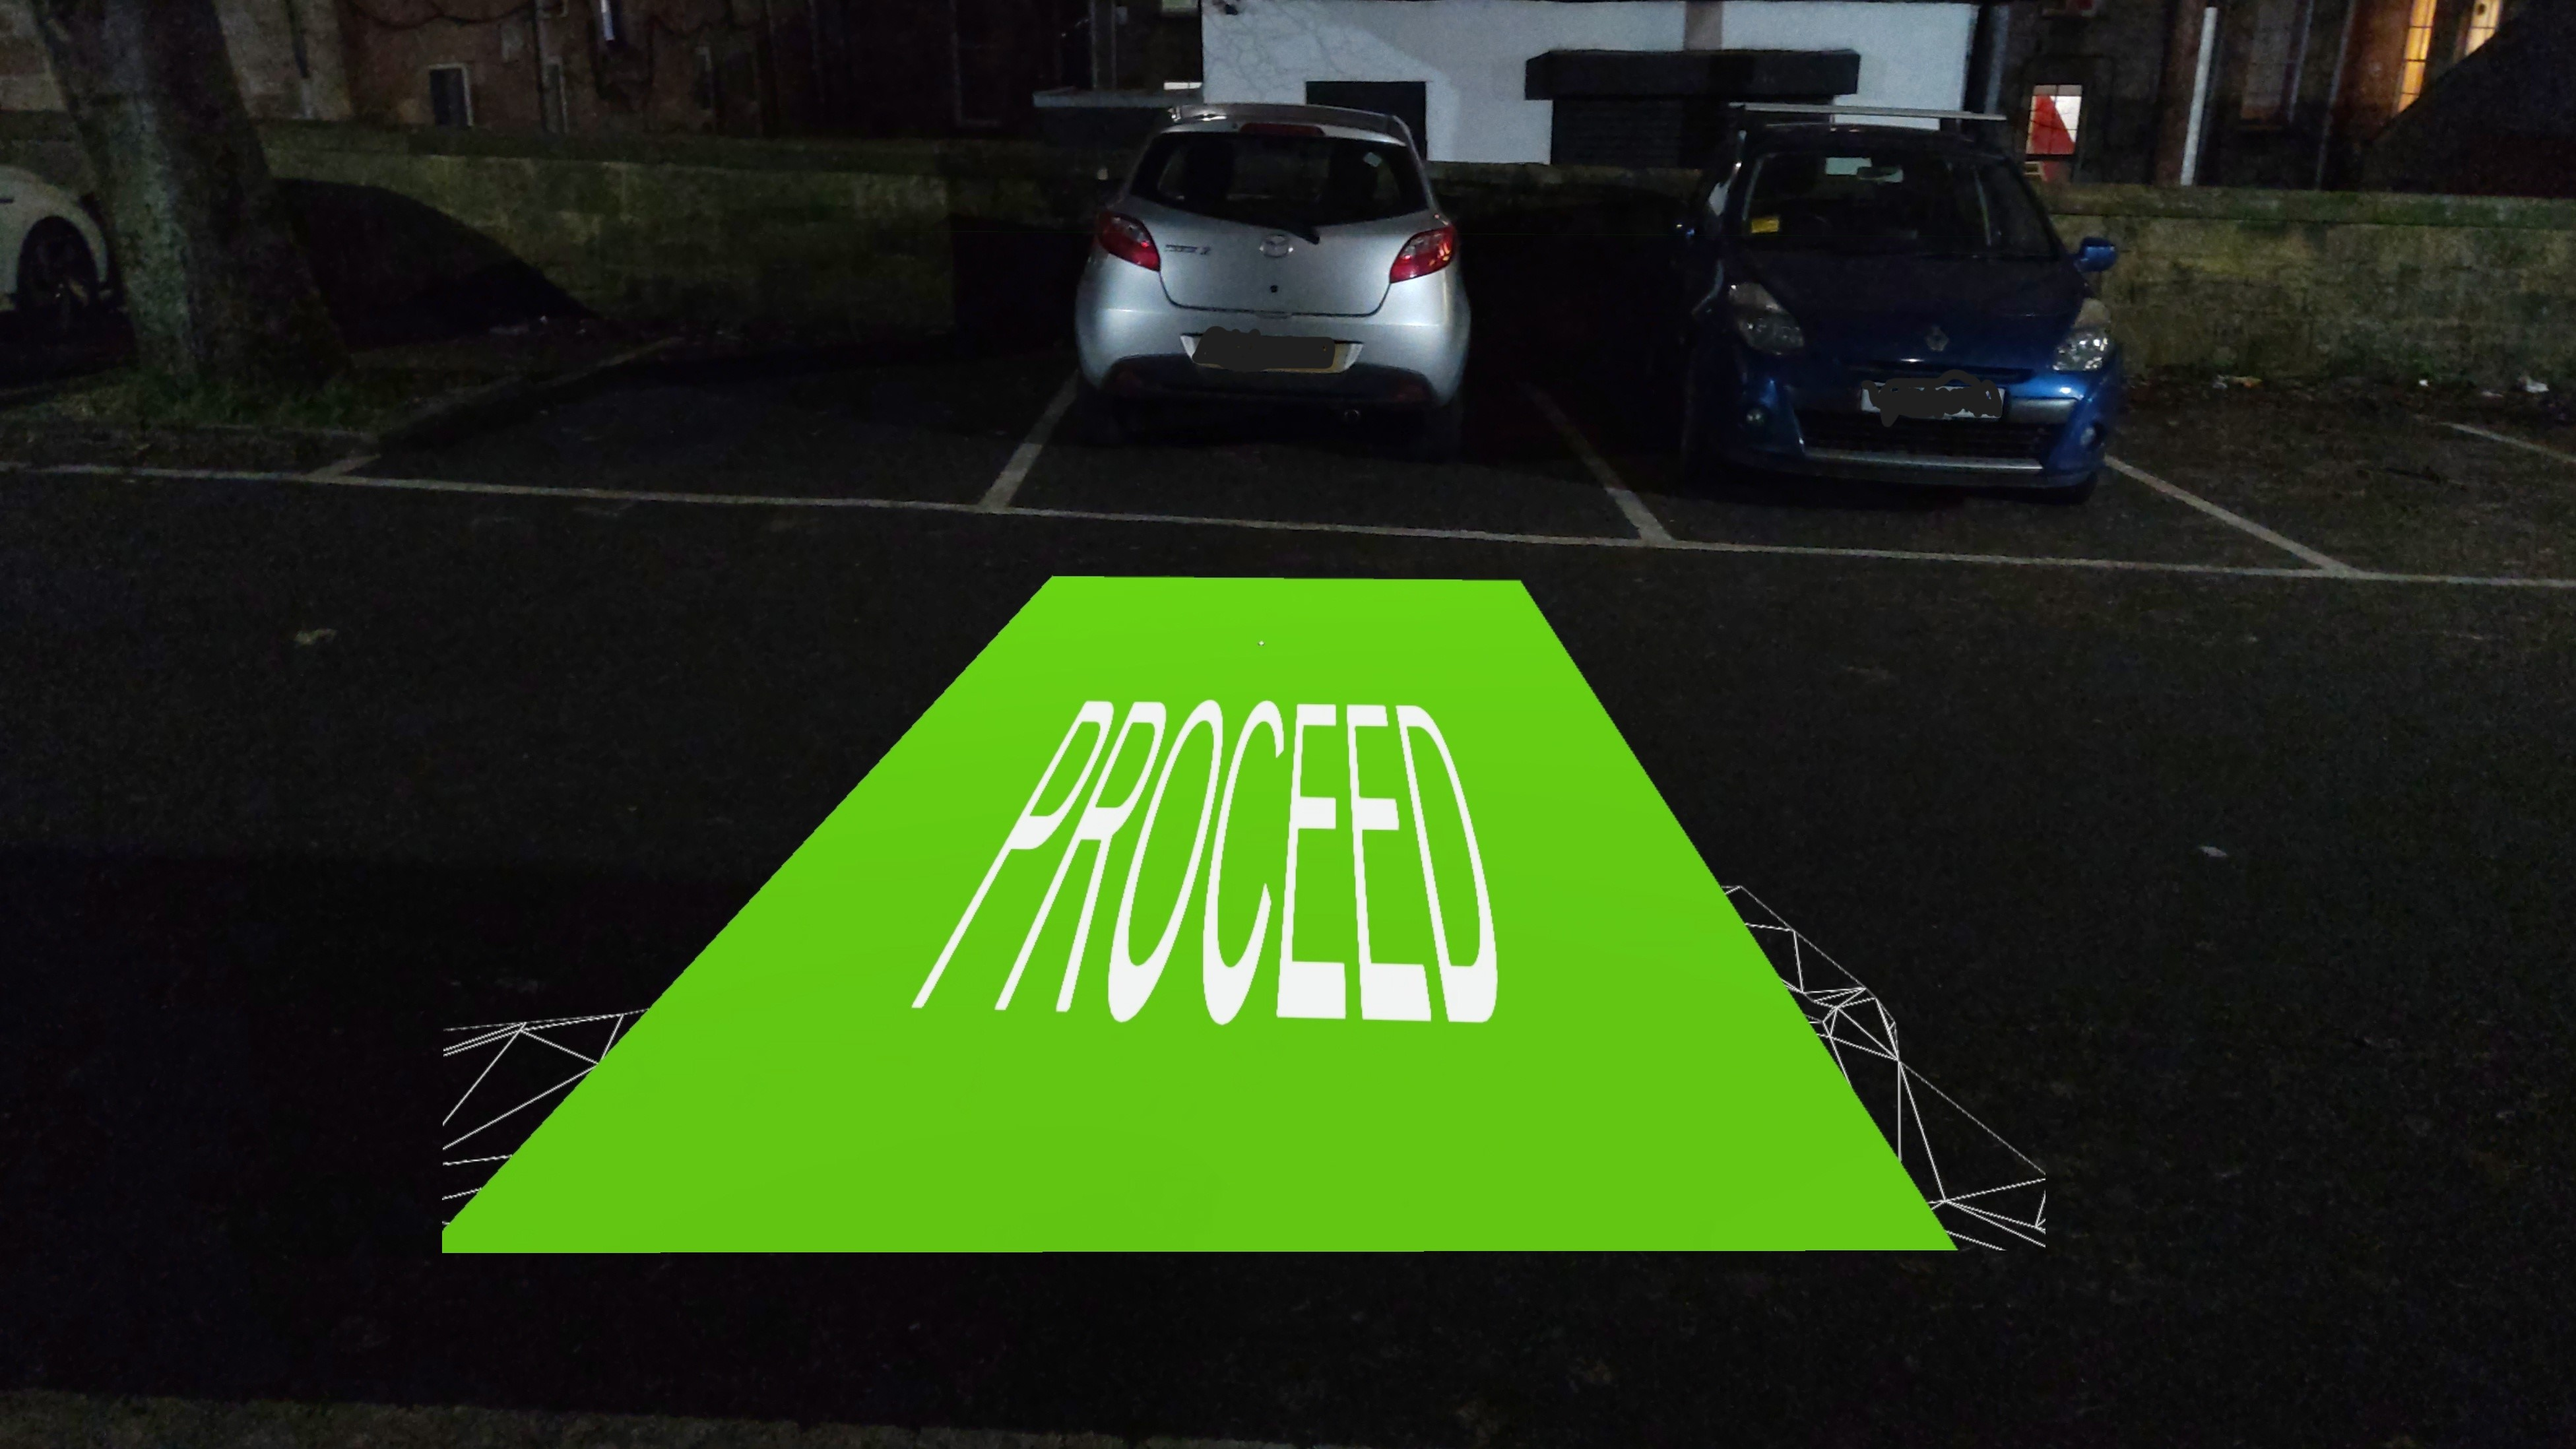
\includegraphics[width=10cm]{images/design2.3.jpg}
    \caption{Rear Design 2 Green.}
    \label{fig:real_rear_6}
\end{figure}

The photographs taken by the HoloLens are evidence of the prototype working as intended, however occasionally errors were ran into when testing was being performed. The issue I discussed earlier surrounding the unreliability of UDP often came into play and regularly the graphic overlays could be seen off target for a second before they would reposition back to the correct position. Despite my requirements stating that the prototype should be able to be used comfortably on a bicycle, I am unsure on the safety of doing so and I am not certain that a cyclist would be able to wear the augmented reality headset for long periods of time.

\section{Survey Design}

Having tested and received mostly positive results from the prototype I was now ready to receive feedback on the prototype and opinion on augmented reality headsets in general from cyclists. To achieve this a study was required to be carried out to gather the necessary evidence. Having looked into several different options, I decided upon using a survey based study which would allow cyclists to give their opinion in an honest manner. I felt it was important to get a true and accurate response from all of the respondents so therefore the survey was made entirely anonymous and no data about the respondents was recorded. This would allow cyclists to be able to speak their mind about the interaction design and the state of cyclist-autonomous vehicle interaction in general. To create the survey, Google Forms was used as it allows for an easy setup of surveys and correlates the responses in a format that makes analysis uncomplicated.

The survey was split up into six different sections which allowed respondents to focus on specific sections at a time. For the first four sections the survey focused on gaining opinion on the interaction designs created for the prototype. The images taken by the HoloLens were used and participants were briefed on the scenario and how the design works. The survey then shows them the images taken from the HoloLens and asks for their preference of design, either design one or two for the side and rear designs. This allows for a better understanding of which design would be preferred by cyclists when out on the road wearing the augmented reality headset. To further this understanding, the participants are then asked a follow up question which asks why they chose the specific design they did. In this question we are attempting to leverage more information from the respondents about why in particular they preferred the design, the information gathered here may help inform on future design choices.

In the last two sections, general questions are asked that are associated with the topic area. The first question asks 'How do you feel about the idea of wearing an augmented reality headset while cycling?'. In this question we want to know whether or not cyclists could see themselves wearing an augmented reality headset whilst cycling on public roads in the future. Responses could help to indicate whether or not the area should be researched more in the coming years.

In the second question we ask respondents 'What concerns or reservations do you have about using augmented reality technology while on the road?'. This allows the participants to provide further detail about opinions they may have on the issues of wearing a headset. In particular, it may help to highlight areas of issue that are relevant to cyclists that could be addressed in the future.

Thirdly, we ask 'Based on your current knowledge and perceptions, do you see augmented reality as a positive or negative addition to cycling safety?'. Again, we wish to gather more information on the general thoughts towards adding augmented reality to cycling. Much like the previous question, the participants response will help to gauge whether further research is worthwhile in the area.

Finally, in the last question we ask 'Any design suggestions you have for ways which cyclists and drivers may interact?'. This question is more relevant towards the interactions with drivers but is still relevant when looking at interactions with autonomous vehicles. The responses here will indicate any themes amongst cyclists of possible communication methods they would like to see potentially trialed in the future.

To find participants to complete this anonymous survey, the social media platform Reddit was used. Reddit is a platform that allows the creation of 'Subreddits' or communities of people who share interests. In the case of this study, it was important to get responses from cyclists who spent a lot of time cycling, mainly on public roads where they interact with vehicles. It was also important however to ensure that I got a rounded opinion from the cycling community so the selection of 'Subreddits' that I posted the survey in was critical to ensuring a good coverage of all types of cyclist. The 'Subreddits' I posted my survey in consisted of 'r/bikecommuting' and 'r/ukbike'.

\section{Results}

\subsection{Overview}

Over the course of several weeks I managed to obtain 15 different respondents to my survey. As I collected no information from the participants, there is no way of knowing whether the respondents are avid cyclists who cycle everyday or less active cyclists who cycle a couple of times a year. However, considering the 'Subreddits' I chose to post the survey in I feel confident in the pool of respondents that completed the survey being diverse enough to give a good representation of the cycling communities opinion as a whole.

\subsection{Side View Design}

\begin{figure}[htbp]
    \centering
    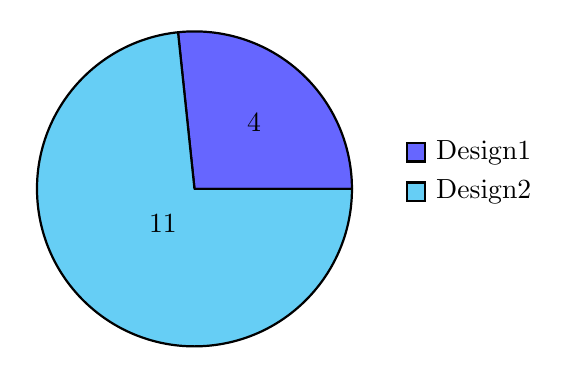
\begin{tikzpicture}
        \pie[text=legend, sum=auto, radius=2]{4/Design1, 11/Design2}
    \end{tikzpicture}
    \caption{Preferences of Design for Side View.}
    \label{fig:pie_chart1}
\end{figure}

As you can see in the Figure \ref{fig:pie_chart1}, the majority of respondents preferred the second design with the wording involved to further convey the message.

Although there was less support for the first design, respondents cited two reasons they preferred the simpler design with no wording. Two respondents stated that they thought reading the words could be distracting, whilst the other two said that they felt the words were instructing them to perform an action rather than informing them of something happening.

Despite having more supporters, the main reasoning behind the decision to support the second design was down to two factors. All of the respondents who voted for design two felt it was clearer and easier to understand, with half of them citing the fact that the wording solves the issue regarding colour blindness.

\section{Rear View Design}

\begin{figure}[htbp]
    \centering
    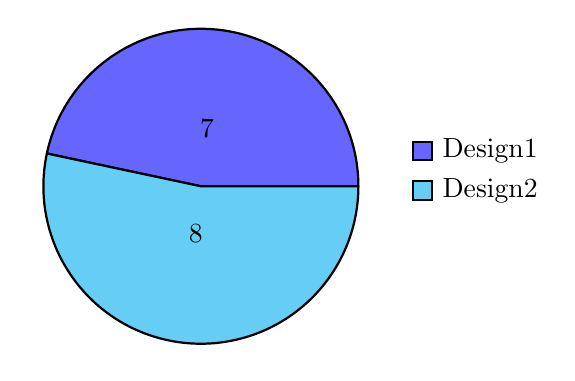
\begin{tikzpicture}
        \pie[text=legend, sum=auto, radius=2]{7/Design1, 8/Design2}
    \end{tikzpicture}
    \caption{Preferences of Design for Rear View.}
    \label{fig:pie_chart2}
\end{figure}

Figure \ref{fig:pie_chart2} represents the voting for preference of design for the rear view. This time there is insufficient evidence to declare a preferred design as the votes are split across both designs.

Reasoning behind voting for the first design followed a similar pattern for the reasons behind voting for the first side view design. Some respondents thought that the wording would distract them their surroundings, whilst others indicated that they would rather be informed about something than instructed on what to do in a certain situation.

In a similar vein, the reasons respondents told us they voted for design two was very similar to the reasons behind voting for the second design in the side view interaction. They felt that the wording gave a clearer message that could be understood better and several cited, once again, about the colour blindness issue.

\subsection{General Questions}

\subsubsection{How do you feel about the idea of wearing an augmented reality headset while cycling?}

Responses to this question were very mixed. Several participants indicated that they would be intrigued by the usage of augmented reality headsets but a theme amongst all the positive responses was that of hesitancy towards it. Some of the positive responses stated that they were excited about the prospect of technology creating a safer environment on public roads but indicated that they felt that this approach was not the right idea. In the negative responses various themes emerged, some cited the fact that they thought this would be an expensive way to solve the problem, some worried about weather and sweat interfering and damaging the headset, and some refrained from providing context but simply did not like the idea of wearing augmented reality headsets.

\subsubsection{What concerns or reservations do you have about using augmented reality technology while on the road?}

Participants gave responses with a wide variety of concerns they had towards the usage of augmented reality technology. A couple of the responses centred around the concern that the headset would be distracting from understanding their surroundings and some went as far to say that they felt it would do more harm than good. A few participants indicated having concerns about being able to use the headset for longer lengths of time, either due to battery life, weather or the comfort of wearing the headset. Several indicated that they felt as though the wearing of the headset would just become another tool to be blamed for if they had an accident whilst cycling.

\subsubsection{Based on your current knowledge and perceptions, do you see augmented reality as a positive or negative addition to cycling safety?}

Again, responses were fairly mixed in answer to this question. A lot of the participants refused to elaborate on why they saw augmented reality as a positive or negative addition, however the few that did offered varied reasons why. One participant stated they had a positive view on the addition of augmented reality because they felt there could be applications in the future for poor visibility conditions and the general communication with self driving vehicles. Others stated negative responses due to pricing and the feeling, once again, that it would place the burden of being safe on the cyclist rather than the autonomous vehicle. They further stated that autonomous vehicles should not be out on the road if they cannot operate safely with all road users.

\subsubsection{Finally, any design suggestions you have for ways  which cyclists and drivers may interact?}

Once again, responses were very varied for this question with some giving valuable suggestions for interaction design and others choosing to state the need for separate cyclist infrastructure entirely. Some interesting responses included the suggestion of cyclists returning to using hand signals if an autonomous vehicle could be made to recognise them, whilst others suggested sticking to something more simple such as lights being displayed on a vehicle, rather similar to the suggestion given in 'Keep It Real'.

\section{Discussion}

Perhaps understandably, the views stated from the cyclists that participated in the survey are extremely varied. Results from the survey do not give any encompassing opinions that all cyclists share and instead offer a variety of themes of which all matter in varying degrees to each of the participants. There is however a significant amount of participants who believe that the usage of augmented reality headsets places the burden of safety on the cyclist rather than the autonomous vehicle which is several times the size of them. These participants also responded with suggestions of creating an entirely separate cycling infrastructure that would see cyclists and vehicles use different roads to ensure safety. Whilst it was not the goal of the study to look into this area, the support received in the servery was significant and I therefore believe it does need to be highlighted.

Of those that responded positively to the idea of using augmented reality headsets whilst cycling, several voiced concerns for a varied number of reasons. These concerns were all justifiable and highlight areas that potential future studies may address such as the possibility of being distracted by the headset whilst cycling. The concerns regarding cost and capabilities of headsets, whilst also valid, can generally be brought down to the current day and age. In years to come it is not hard to believe that the capabilities, i.e. battery size and weatherproofing, will increase exponentially whilst the cost of units will hopefully come down as more and more money is funnelled into the augmented reality industry. But for that to happen there needs to be a considerable interest in the area and the results here show that, whilst not always positive, there is a significant amount of interest towards the adoption of technology in order to make the world a safer place.

%==================================================================================================================================
\chapter{Conclusion}    

To conclude, the main objective of this study was to look into a solution to the upcoming problem of communication between autonomous vehicles and cyclists. With the eventual adaptation of driverless vehicles into society, other road users including cyclists who rely on the social and implicit cues given by drivers, will face issues when understanding intent and the awareness of autonomous vehicles. This break in communication could potentially make cycling on public roads unsafe and, without a solution, would effect the millions of people who cycle to and from work daily.

To address the problem, I designed and built a prototype that would allow cyclists to receive information from an autonomous vehicle out on the road. The prototype was built using a Zed 2 stereo camera to handle the vehicle detection, a HoloLens 2 to display the different graphic overlays that I designed and makes use of UDP to communicate the data. The prototype was then tested on a stationary car where it achieved the goals set out for the project by detecting the vehicles position and displaying the graphics through the headset. The evaluation of the prototype was performed by conducting a survey to receive information on design preferences and cyclists overall opinion on augmented reality technology.

The results from the study found that, in general, cyclists opinions on interaction design and using augmented reality to increase their safety whilst riding on public roads was fairly mixed. Most highlighted the need for words to be used in designs as it allows colourblind people to understand better, however some stated that the words would be distracting and too much to focus on when cycling. Perhaps, in order to compromise this could me made into a setting if any future work is carried out. Respondents who were intrigued by the usage of technology in road safety also had concerns about ensuring levels of concentration, battery level, the comfort of the headset and the effect weather and sweat might have on the device. A common theme for concern was the cost that augmented reality headsets are priced at, however as stated previously this is sure to lower and become  more commercially viable as interest in the headsets grow. Those who were opposed to the idea of implementing augmented reality technology into their daily rides, mainly did so due to feeling like it would be just another tool to be blamed on by vehicle owners. As a counter point, cyclists who opposed the idea of wearing the headset mainly suggested that autonomous vehicles should not be on the road if they are not safe. They also suggested the idea of creating entirely different cycling infrastructure to ensure the two parties never meet.

Looking back on the project, if I had more time I would have liked to get the YOLO algorithm working. This would allow for a simpler solution as an external object detection device would not be necessary and would make the prototype closer to what a real world product may look like in the future. I would have also liked to get the prototype trialed by cyclists in a real world study, this was not possible due to encountering comparability issues with object detection and therefore having a shorter amount of time to complete the project.

Future studies may look into trialing a complete prototype in a real world scenario, a cyclist performing their morning commute perhaps. I do however think it is imperative that a larger study is done on the opinion of cyclists on autonomous vehicles, as a large portion of them were very adverse to the idea of sharing a road with them and some offered the idea, as previously mentioned, of separating cyclists and vehicles entirely.

In essence, this study emphasises the importance of addressing the communication gap between cyclists and autonomous vehicles to ensure road safety for everyone.

%==================================================================================================================================
%
% 
%==================================================================================================================================
%  APPENDICES  

\begin{appendices}

\chapter{Appendices}

Screenshots of the survey.

\begin{figure}[H]
    \centering
    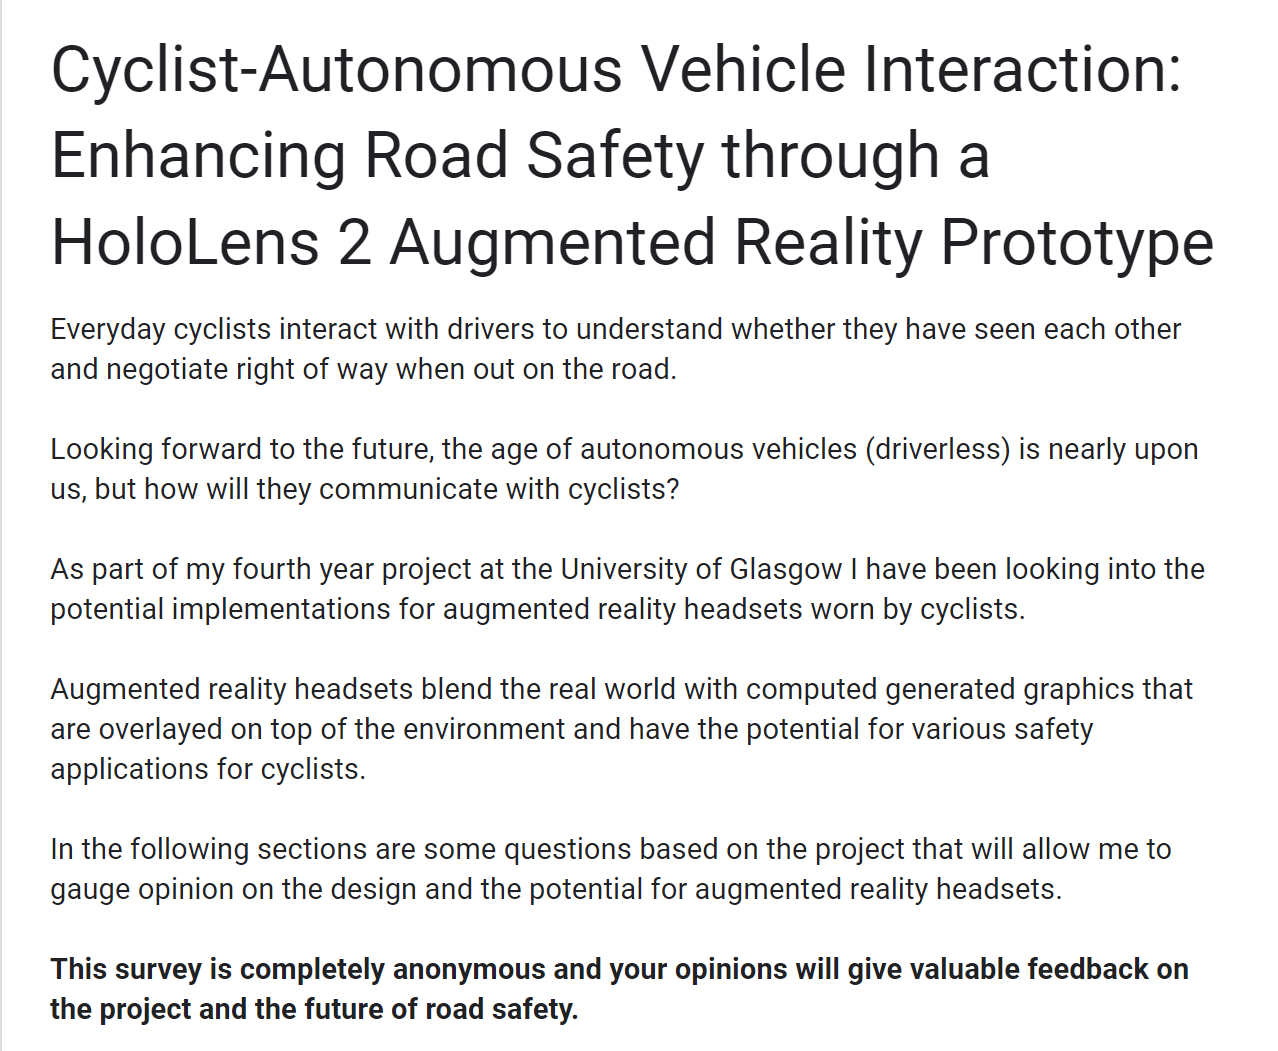
\includegraphics[width=10cm]{images/survey1.png}
    \caption{Survey Briefing.}
    \label{fig:survey1}
\end{figure}

\begin{figure}[H]
    \centering
    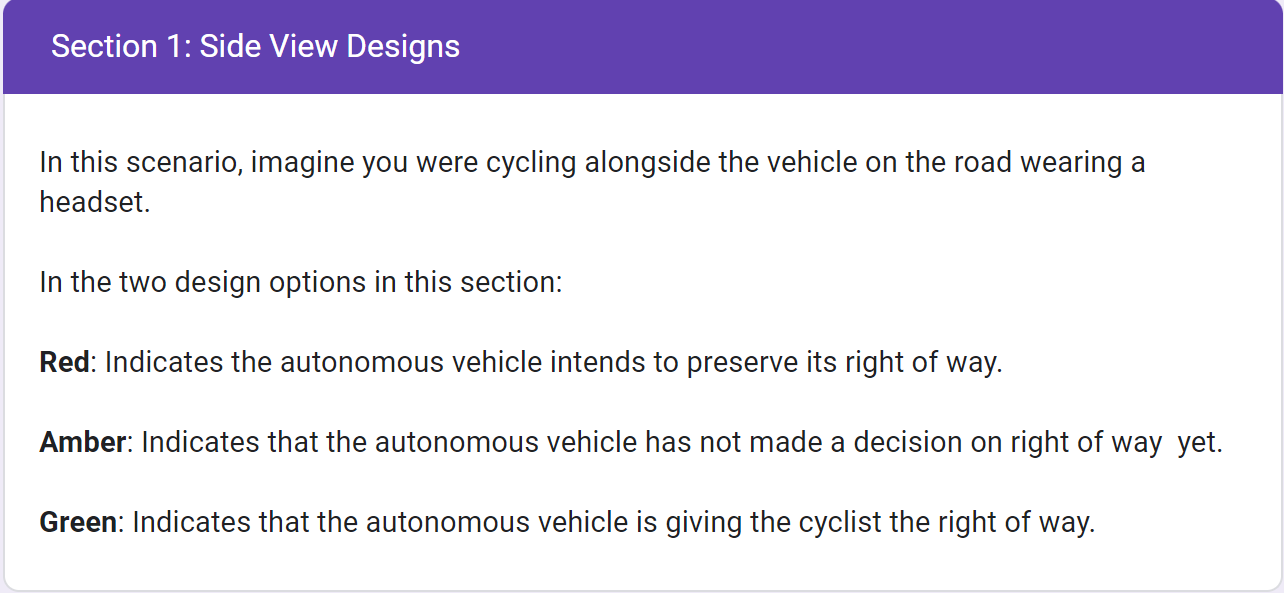
\includegraphics[width=10cm]{images/survey2.png}
    \caption{Survey First Questions Briefing.}
    \label{fig:survey2}
\end{figure}

\begin{figure}[H]
    \centering
    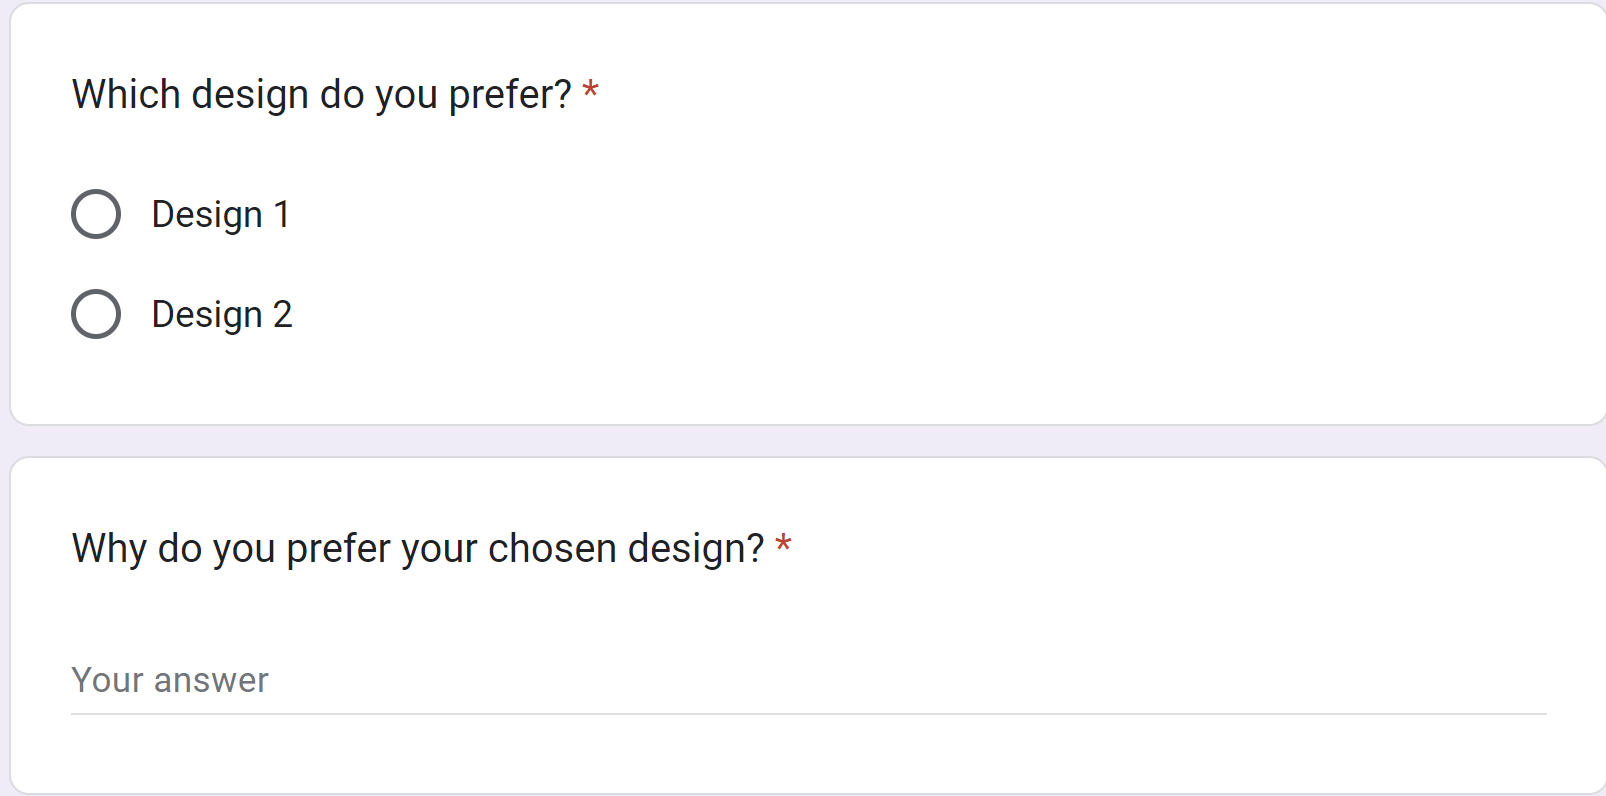
\includegraphics[width=10cm]{images/survey3.png}
    \caption{Answer Section of First Questions.}
    \label{fig:survey3}
\end{figure}

\begin{figure}[H]
    \centering
    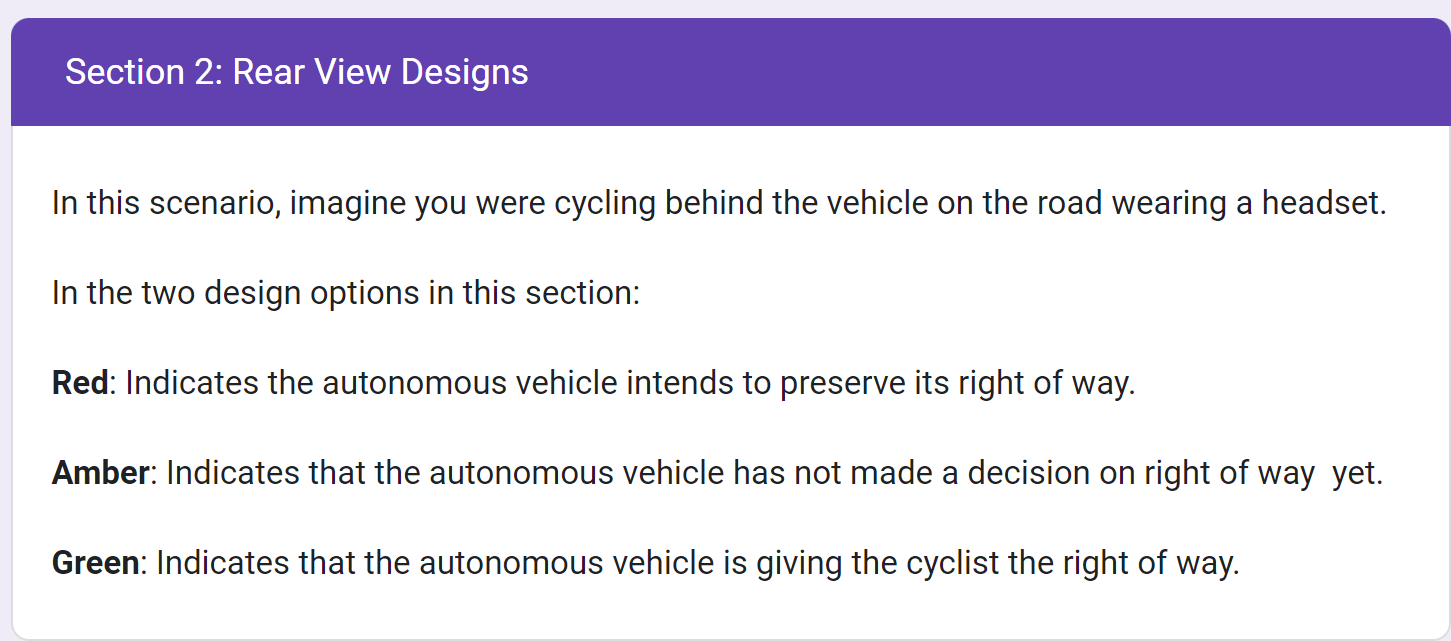
\includegraphics[width=10cm]{images/survey4.png}
    \caption{Survey Second Questions Briefing.}
    \label{fig:survey4}
\end{figure}

\begin{figure}[H]
    \centering
    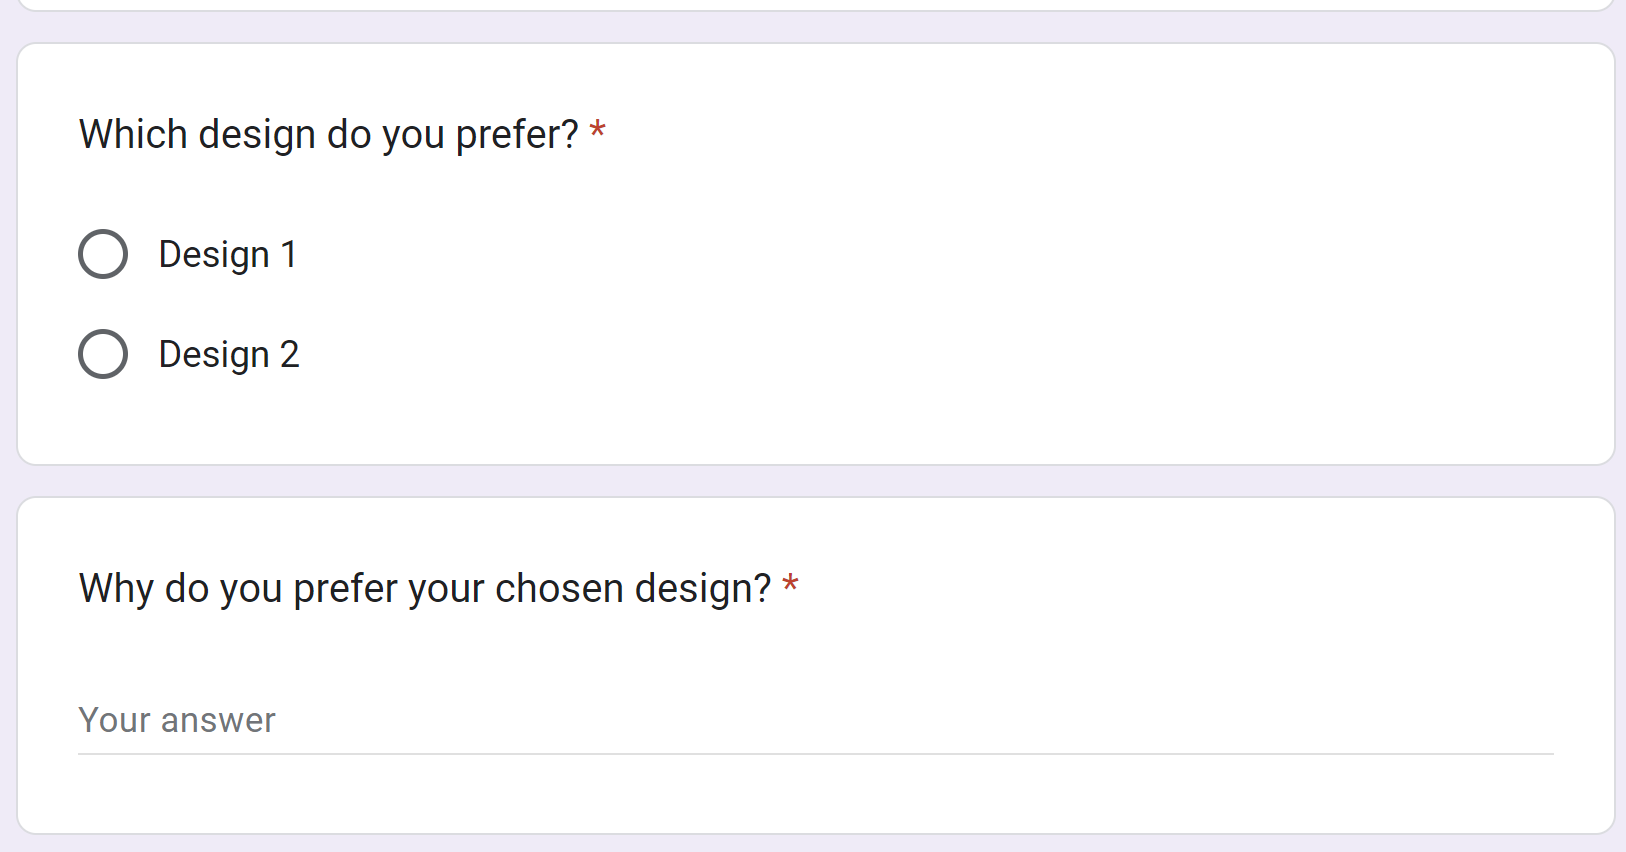
\includegraphics[width=10cm]{images/survey5.png}
    \caption{Survey Section of Second Questions.}
    \label{fig:survey5}
\end{figure}

\begin{figure}[H]
    \centering
    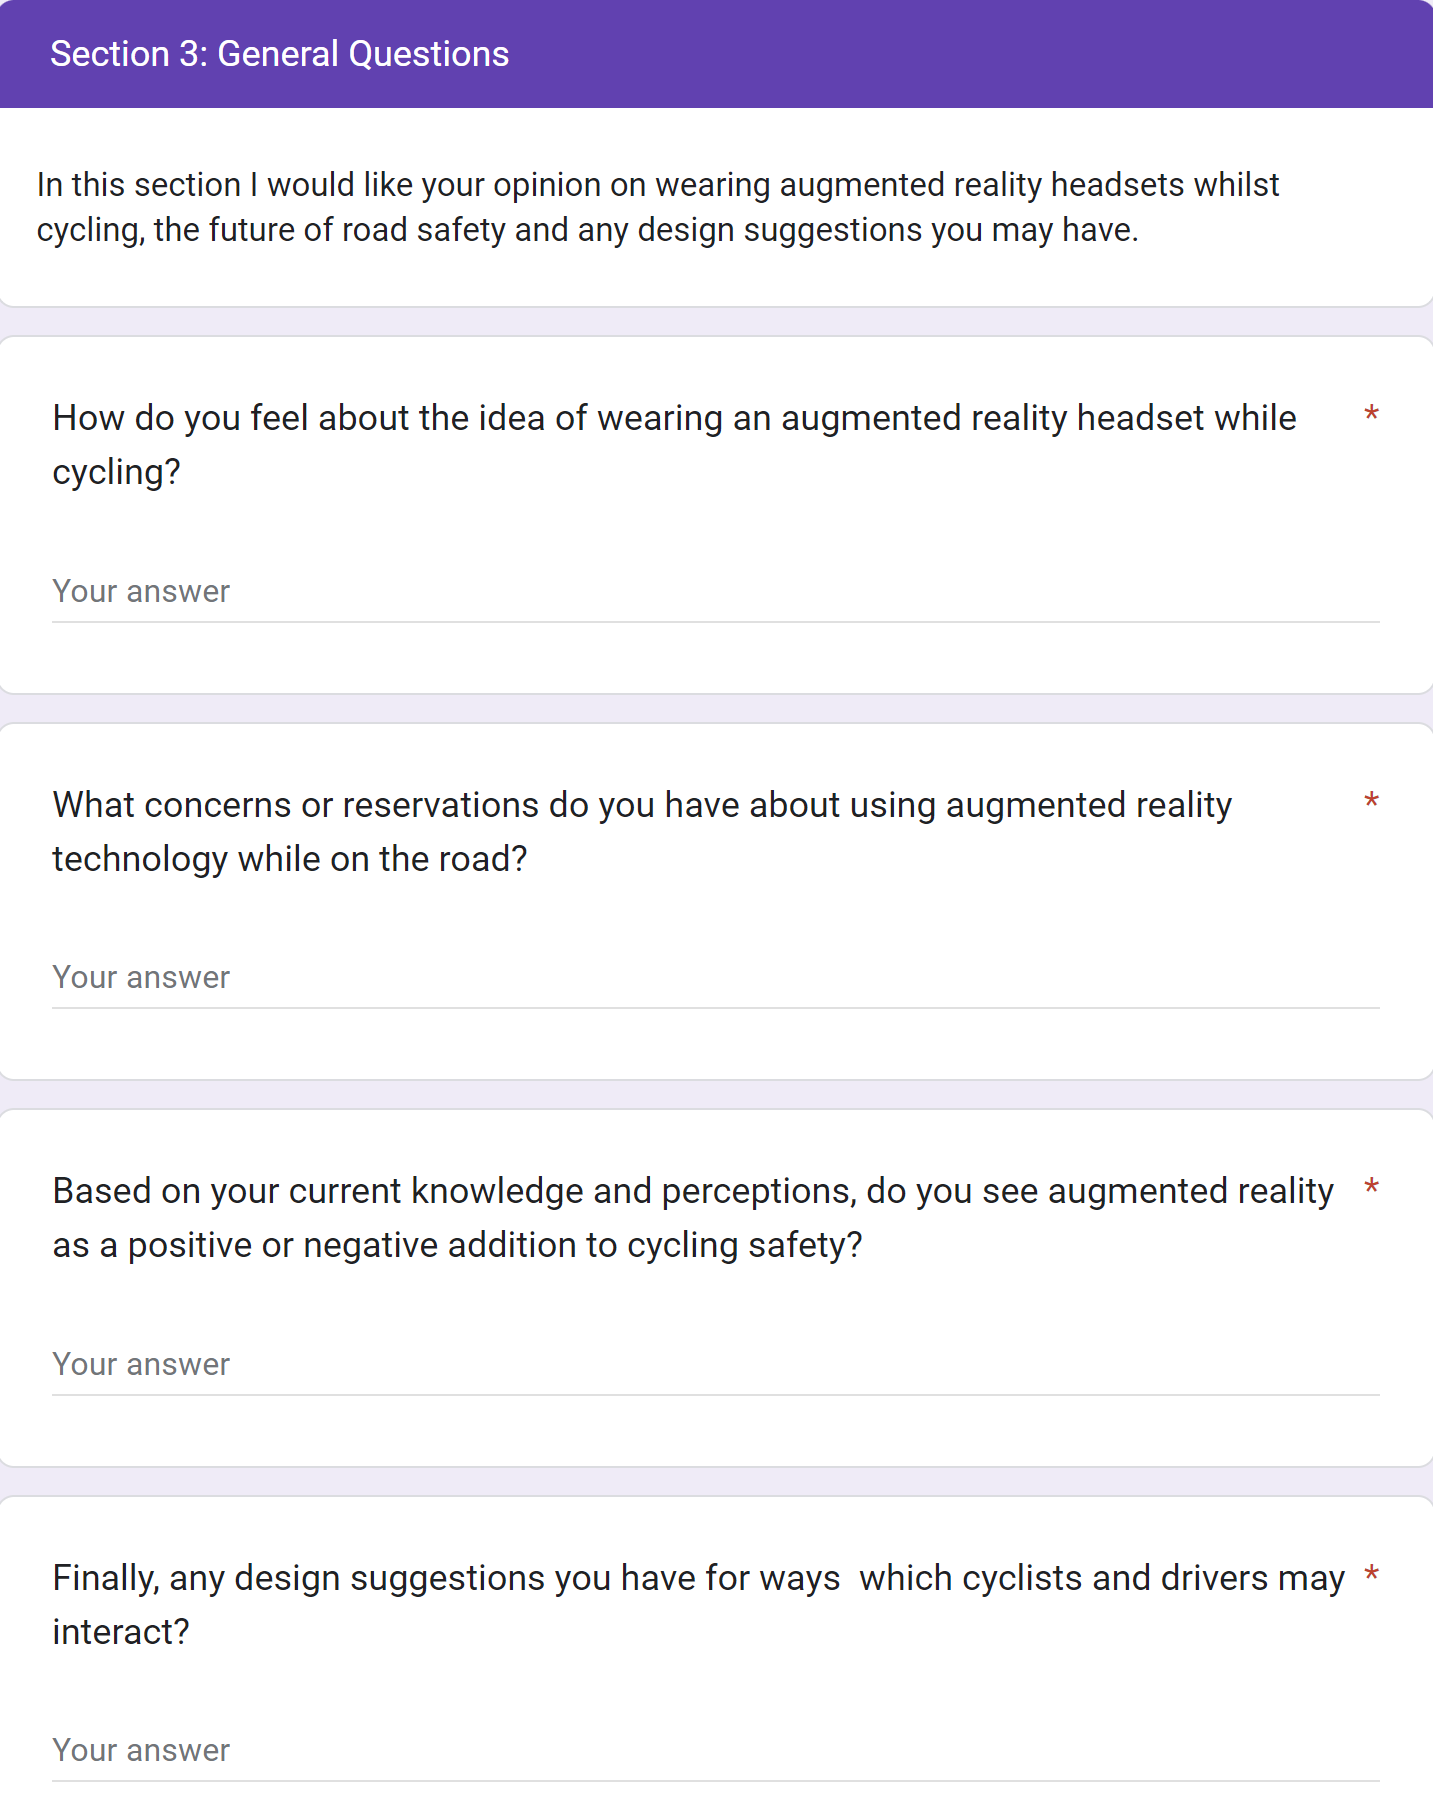
\includegraphics[width=10cm]{images/survey6.png}
    \caption{Survey General Questions.}
    \label{fig:survey6}
\end{figure}

\end{appendices}

%==================================================================================================================================
%   BIBLIOGRAPHY   

% The bibliography style is abbrvnat
% The bibliography always appears last, after the appendices.

\bibliographystyle{abbrvnat}

\bibliography{l4proj}

\end{document}
